\documentclass[12pt]{extarticle}
\usepackage[paperwidth=15in,paperheight=7.2in]{geometry}
\usepackage{amsmath}
\usepackage{hyperref}
\usepackage{multirow}
\usepackage{pdfpages}
\usepackage[utf8]{inputenc}
\title{Kaon mixing: chiral and continuum extrapolations}
\author{R Mukherjee}
\date{\today}
\begin{document}
\maketitle
\tableofcontents
\clearpage
\begin{figure}
\centering
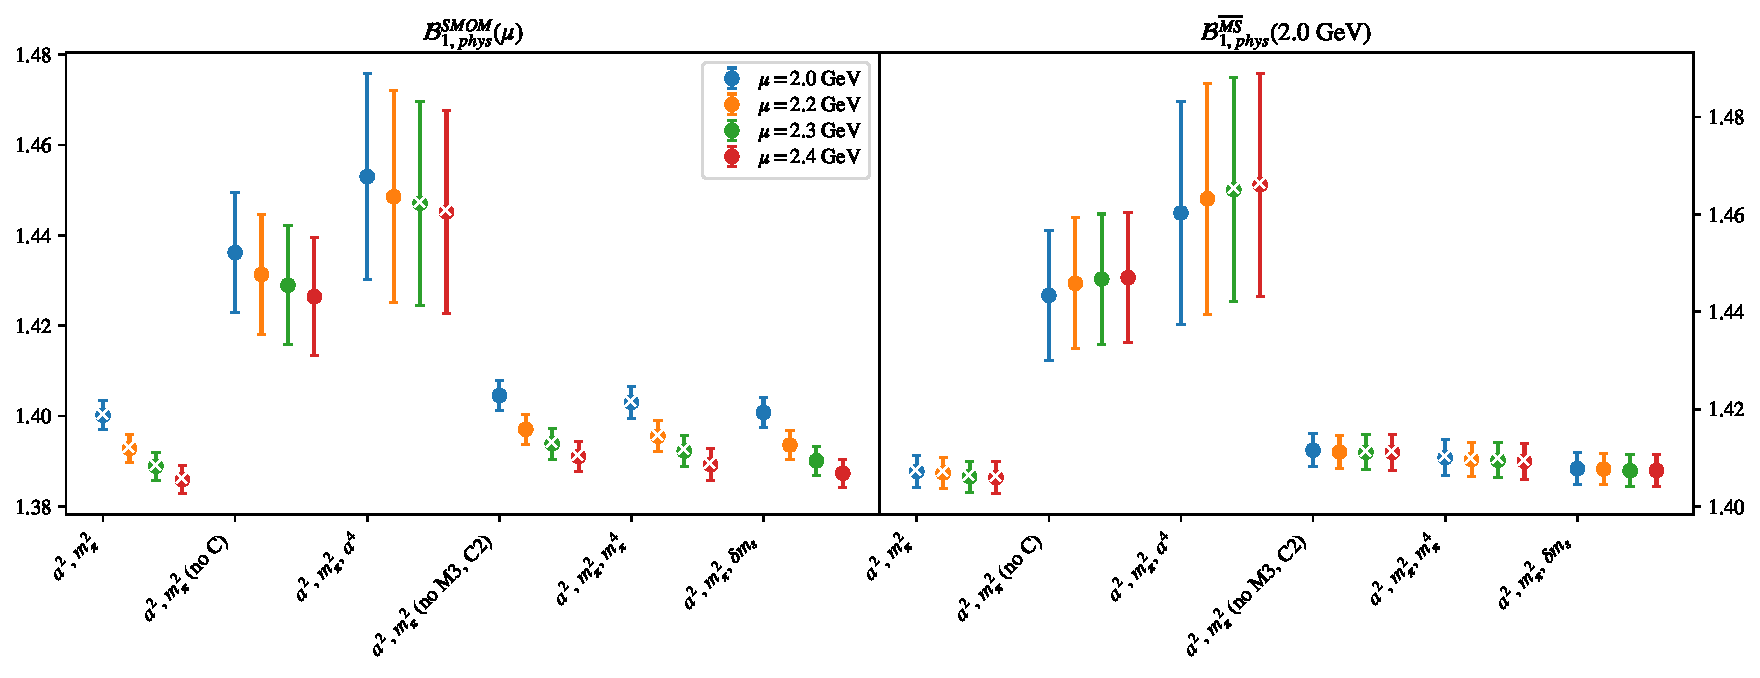
\includegraphics[page=1, width=1.1\textwidth]{VVpAA/NPR/fit_summary_bag.pdf}
\caption{$\mathcal{B}_{1}$\\(left) $\mathcal{B}_{phys}$ in RI/SMOM scheme from fit variations (fits with $p$-value $<0.05$ marked with ``$\times$"). \\(right) $\mathcal{B}_{phys}$ in $\overline{MS}$ computed using $\mathcal{B}^{\overline{MS}} = R^{\overline{MS}\leftarrow SMOM}(2.0)\sigma_{npt}(2.0,\mu) \mathcal{B}^{SMOM}(\mu)$.}
\end{figure}
\clearpage
\begin{figure}
\centering
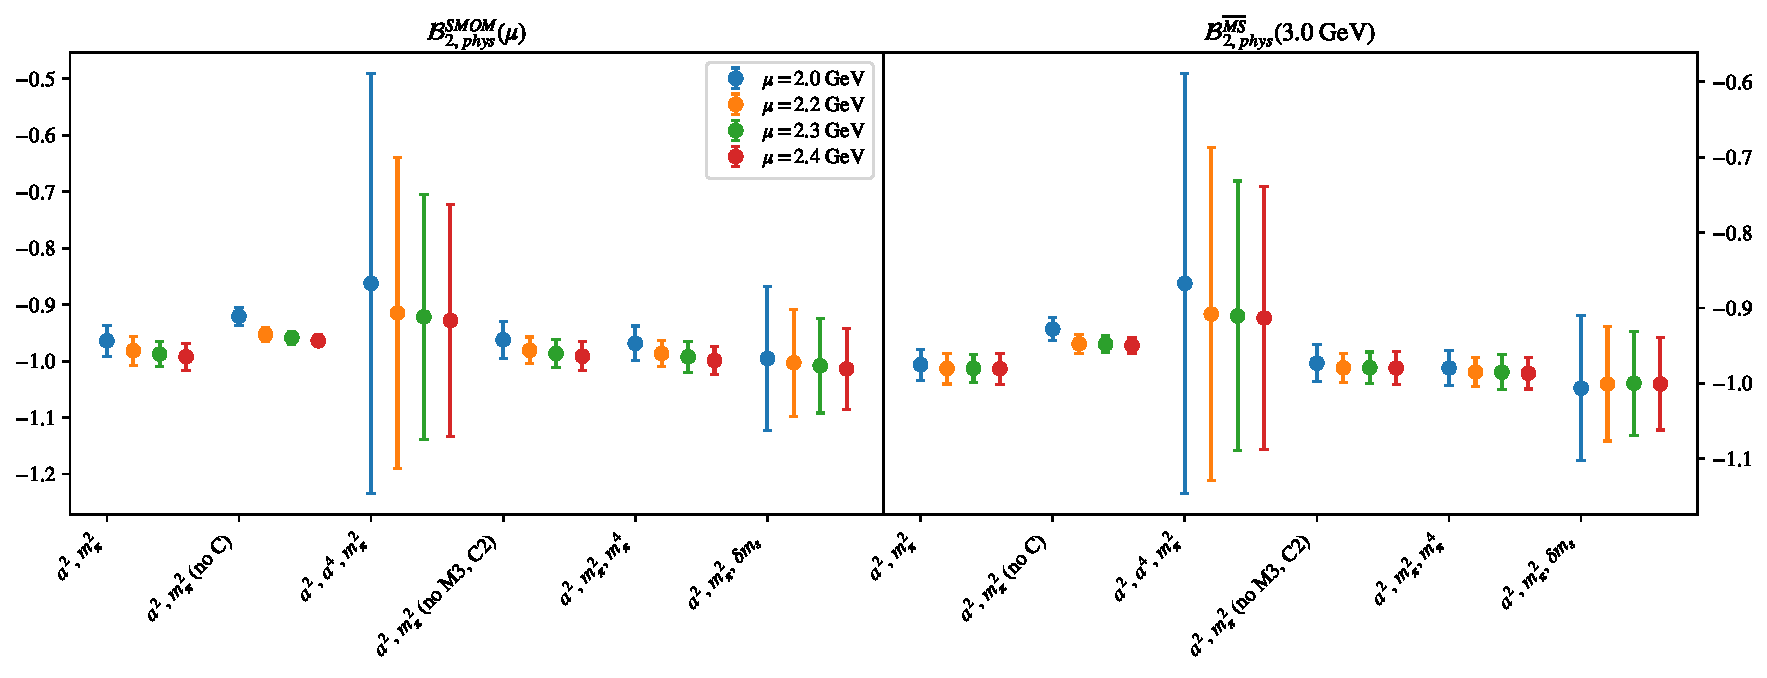
\includegraphics[page=1, width=1.1\textwidth]{VVmAA/NPR/fit_summary_bag.pdf}
\caption{$\mathcal{B}_{2}$\\(left) $\mathcal{B}_{phys}$ in RI/SMOM scheme from fit variations (fits with $p$-value $<0.05$ marked with ``$\times$"). \\(right) $\mathcal{B}_{phys}$ in $\overline{MS}$ computed using $\mathcal{B}^{\overline{MS}} = R^{\overline{MS}\leftarrow SMOM}(3.0)\sigma_{npt}(3.0,\mu) \mathcal{B}^{SMOM}(\mu)$.}
\end{figure}
\clearpage
\begin{figure}
\centering
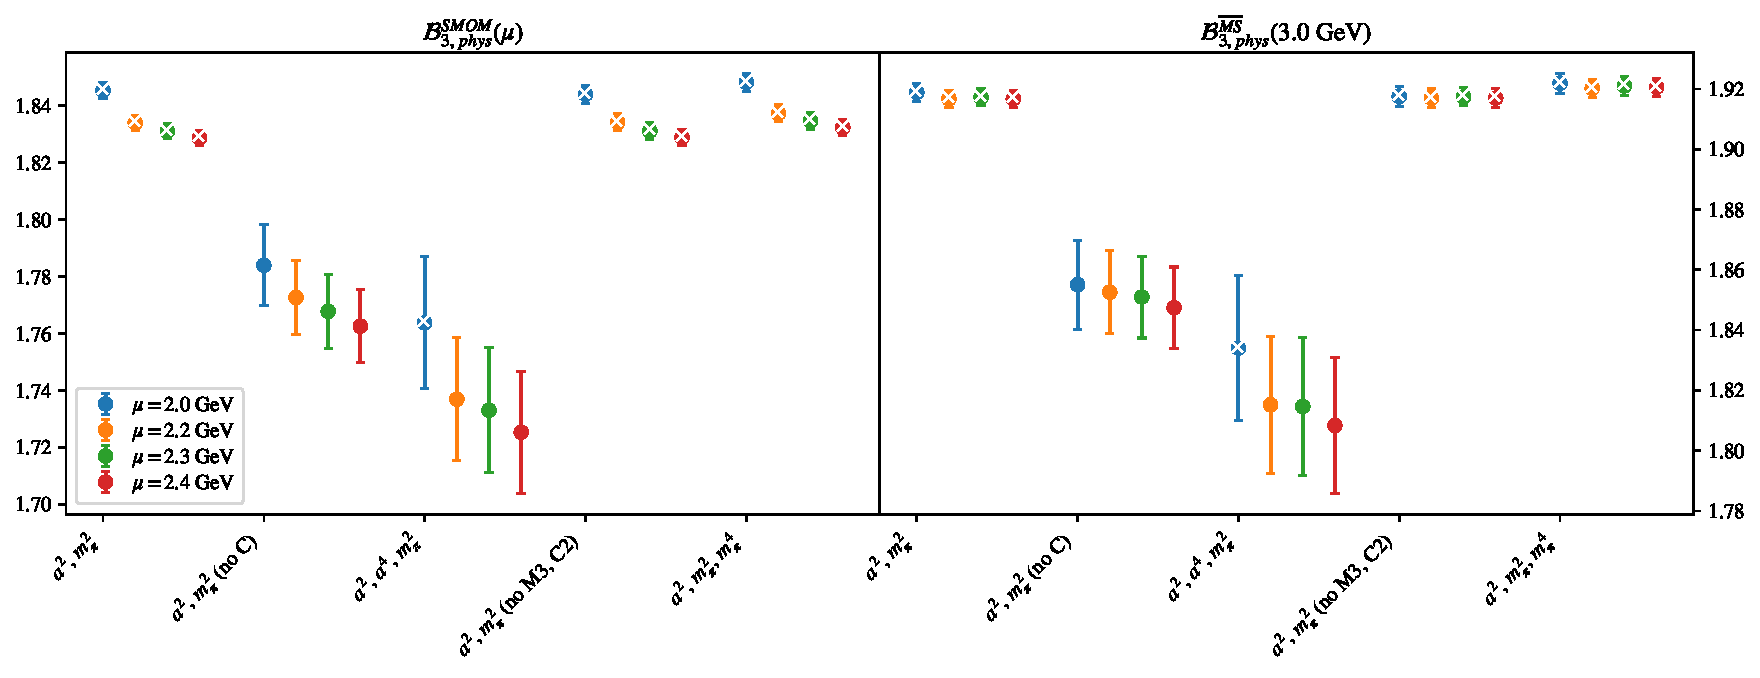
\includegraphics[page=1, width=1.1\textwidth]{SSmPP/NPR/fit_summary_bag.pdf}
\caption{$\mathcal{B}_{3}$\\(left) $\mathcal{B}_{phys}$ in RI/SMOM scheme from fit variations (fits with $p$-value $<0.05$ marked with ``$\times$"). \\(right) $\mathcal{B}_{phys}$ in $\overline{MS}$ computed using $\mathcal{B}^{\overline{MS}} = R^{\overline{MS}\leftarrow SMOM}(3.0)\sigma_{npt}(3.0,\mu) \mathcal{B}^{SMOM}(\mu)$.}
\end{figure}
\clearpage
\begin{figure}
\centering
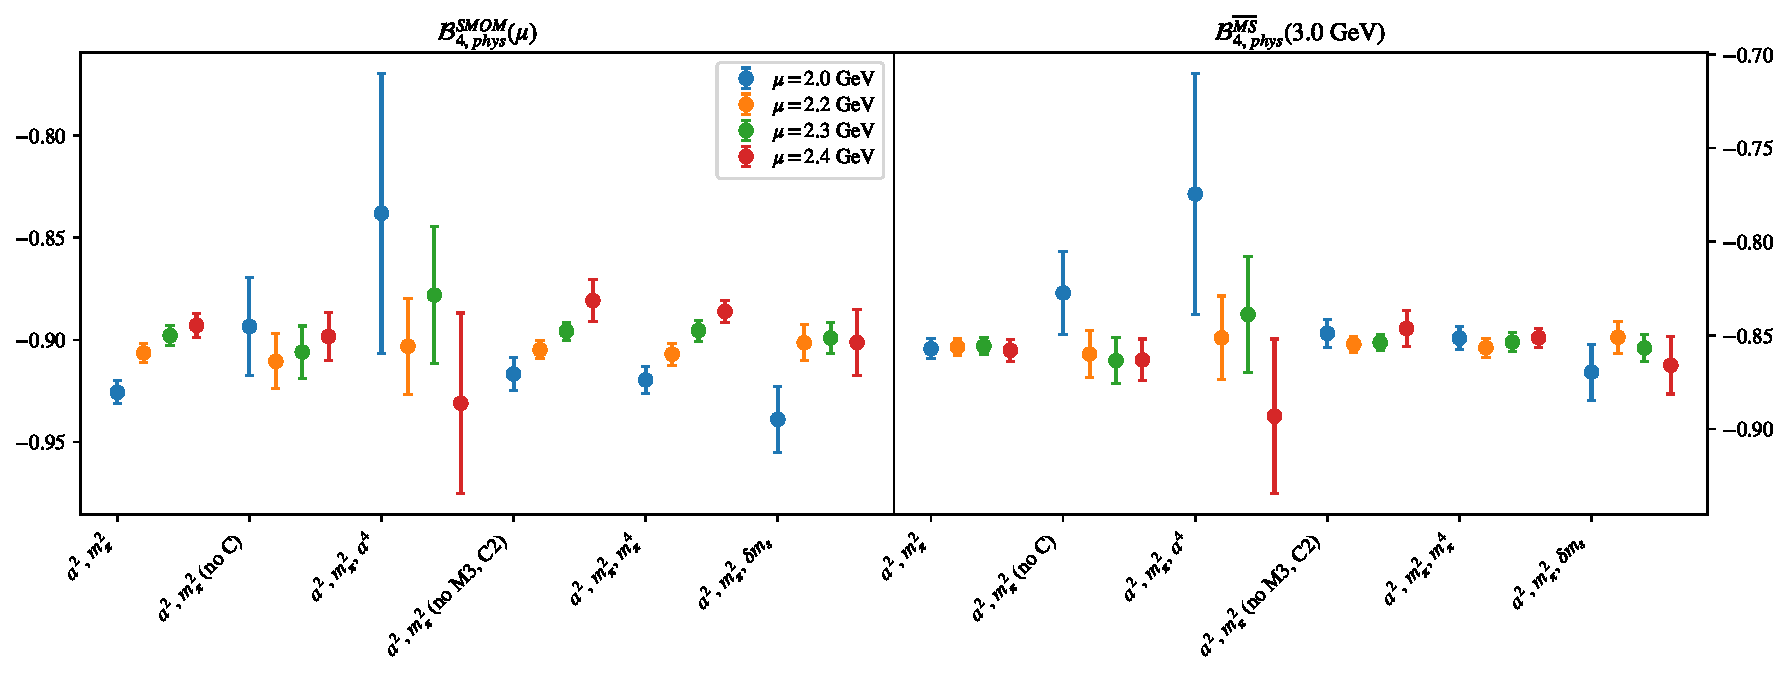
\includegraphics[page=1, width=1.1\textwidth]{SSpPP/NPR/fit_summary_bag.pdf}
\caption{$\mathcal{B}_{4}$\\(left) $\mathcal{B}_{phys}$ in RI/SMOM scheme from fit variations (fits with $p$-value $<0.05$ marked with ``$\times$"). \\(right) $\mathcal{B}_{phys}$ in $\overline{MS}$ computed using $\mathcal{B}^{\overline{MS}} = R^{\overline{MS}\leftarrow SMOM}(3.0)\sigma_{npt}(3.0,\mu) \mathcal{B}^{SMOM}(\mu)$.}
\end{figure}
\clearpage
\begin{figure}
\centering
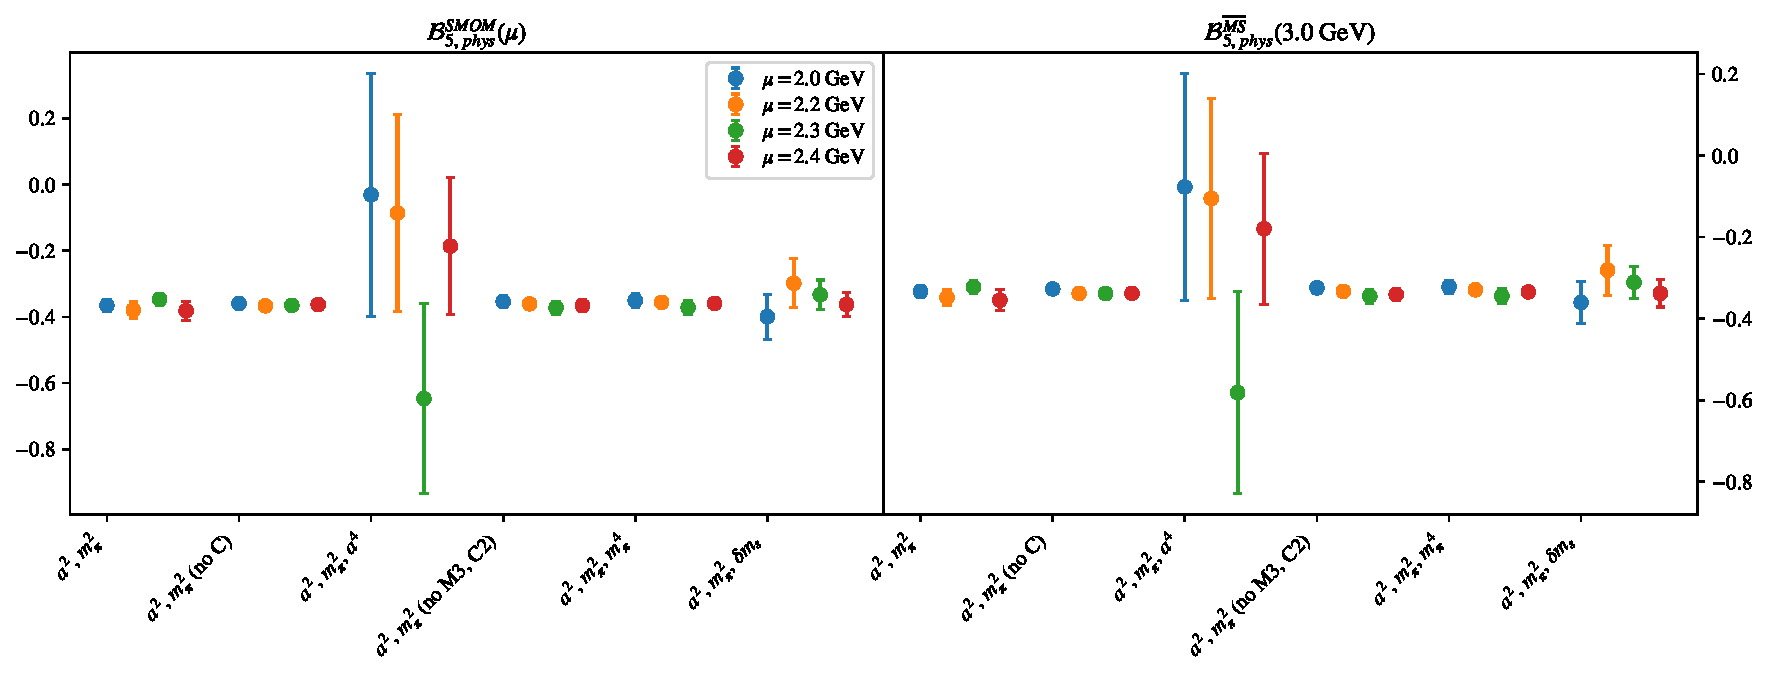
\includegraphics[page=1, width=1.1\textwidth]{TT/NPR/fit_summary_bag.pdf}
\caption{$\mathcal{B}_{5}$\\(left) $\mathcal{B}_{phys}$ in RI/SMOM scheme from fit variations (fits with $p$-value $<0.05$ marked with ``$\times$"). \\(right) $\mathcal{B}_{phys}$ in $\overline{MS}$ computed using $\mathcal{B}^{\overline{MS}} = R^{\overline{MS}\leftarrow SMOM}(3.0)\sigma_{npt}(3.0,\mu) \mathcal{B}^{SMOM}(\mu)$.}
\end{figure}
\clearpage
\section{$\mathcal{B}_1$}
\begin{table}[h!]
\begin{center}
\begin{tabular}{|c|c|c|c|c|c|}
\hline
$\mu$ (GeV) & $a^2$, $m_\pi^2$& $a^2$, $m_\pi^2$ (no C)& $a^2$, $a^4$, $m_\pi^2$& $a^2$, $m_\pi^2$ (no M3, C2)& $a^2$, $m_\pi^2$, $m_\pi^4$\\
\hline
2.0& \hyperlink{VVpAA/NPR/a2m2_20.pdf.1}{\textbf{1.4030(31)}: 2.216 (0.05)} & \hyperlink{VVpAA/NPR/a2m2noC_20.pdf.1}{\textbf{1.415(12)}: 0.978 (0.376)} & \hyperlink{VVpAA/NPR/a2a4m2_20.pdf.1}{\textbf{1.419(21)}: 2.64 (0.032)} & \hyperlink{VVpAA/NPR/a2m2mcut_20.pdf.1}{\textbf{1.4088(35)}: 0.219 (0.883)} & \hyperlink{VVpAA/NPR/a2m2m4_20.pdf.1}{\textbf{1.4090(35)}: 0.733 (0.57)}\\
2.2& \hyperlink{VVpAA/NPR/a2m2_22.pdf.1}{\textbf{1.3957(28)}: 2.513 (0.028)} & \hyperlink{VVpAA/NPR/a2m2noC_22.pdf.1}{\textbf{1.410(12)}: 1.118 (0.327)} & \hyperlink{VVpAA/NPR/a2a4m2_22.pdf.1}{\textbf{1.416(21)}: 2.913 (0.02)} & \hyperlink{VVpAA/NPR/a2m2mcut_22.pdf.1}{\textbf{1.4018(34)}: 0.333 (0.802)} & \hyperlink{VVpAA/NPR/a2m2m4_22.pdf.1}{\textbf{1.4019(34)}: 0.984 (0.415)}\\
2.3& \hyperlink{VVpAA/NPR/a2m2_23.pdf.1}{\textbf{1.3924(28)}: 2.619 (0.023)} & \hyperlink{VVpAA/NPR/a2m2noC_23.pdf.1}{\textbf{1.408(12)}: 1.15 (0.317)} & \hyperlink{VVpAA/NPR/a2a4m2_23.pdf.1}{\textbf{1.414(21)}: 3.011 (0.017)} & \hyperlink{VVpAA/NPR/a2m2mcut_23.pdf.1}{\textbf{1.3986(33)}: 0.383 (0.765)} & \hyperlink{VVpAA/NPR/a2m2m4_23.pdf.1}{\textbf{1.3987(34)}: 1.086 (0.361)}\\
2.4& \hyperlink{VVpAA/NPR/a2m2_24.pdf.1}{\textbf{1.3896(28)}: 2.655 (0.021)} & \hyperlink{VVpAA/NPR/a2m2noC_24.pdf.1}{\textbf{1.405(12)}: 1.162 (0.313)} & \hyperlink{VVpAA/NPR/a2a4m2_24.pdf.1}{\textbf{1.411(21)}: 3.057 (0.016)} & \hyperlink{VVpAA/NPR/a2m2mcut_24.pdf.1}{\textbf{1.3958(33)}: 0.386 (0.763)} & \hyperlink{VVpAA/NPR/a2m2m4_24.pdf.1}{\textbf{1.3958(34)}: 1.108 (0.351)}\\
\hline
\end{tabular}
\caption{Physical point value from chiral and continuum extrapolation at renormalisation scale $\mu$. Entries are \textbf{value(error)}: $\chi^2/\text{DOF}$ ($p$-value).}
\end{center}
\end{table}
\begin{table}[h!]
\begin{center}
\begin{tabular}{|c c|c|c|c|c|c|}
\hline
$\mu$ (GeV) &  & $a^2$, $m_\pi^2$& $a^2$, $m_\pi^2$ (no C)& $a^2$, $a^4$, $m_\pi^2$& $a^2$, $m_\pi^2$ (no M3, C2)& $a^2$, $m_\pi^2$, $m_\pi^4$\\
\hline
\multirow{2}{0.5in}{2.0} & $\alpha$ & 0.0953(73)& 0.048(53)& -0.014& 0.0816(84)& 0.0816(83)\\
 & $\beta$ & 0.00270(14)& 0.00225(27)& 0.00272(15)& 0.00188(29)& 0.0\\
\hline
\multirow{2}{0.5in}{2.2} & $\alpha$ & 0.0994(70)& 0.042(52)& -0.038& 0.0846(83)& 0.0849(82)\\
 & $\beta$ & 0.00268(14)& 0.00222(27)& 0.00272(14)& 0.00184(28)& 0.0\\
\hline
\multirow{2}{0.5in}{2.3} & $\alpha$ & 0.1009(70)& 0.039(52)& -0.045& 0.0859(83)& 0.0864(82)\\
 & $\beta$ & 0.00268(14)& 0.00220(27)& 0.00272(14)& 0.00183(28)& 0.0\\
\hline
\multirow{2}{0.5in}{2.4} & $\alpha$ & 0.1016(70)& 0.039(52)& -0.044& 0.0864(83)& 0.0870(82)\\
 & $\beta$ & 0.00269(14)& 0.00219(27)& 0.00272(14)& 0.00183(28)& 0.0\\
\hline
\end{tabular}
\caption{Fit values of coefficients in $Q = Q_{phys} + \mathbf{\alpha} a^2 + \mathbf{\beta}\left(\frac{m_\pi^2}{f_\pi^2}-\frac{m_{\pi,PDG}^2}{f_\pi^2}\right) + \ldots$.}
\end{center}
\end{table}
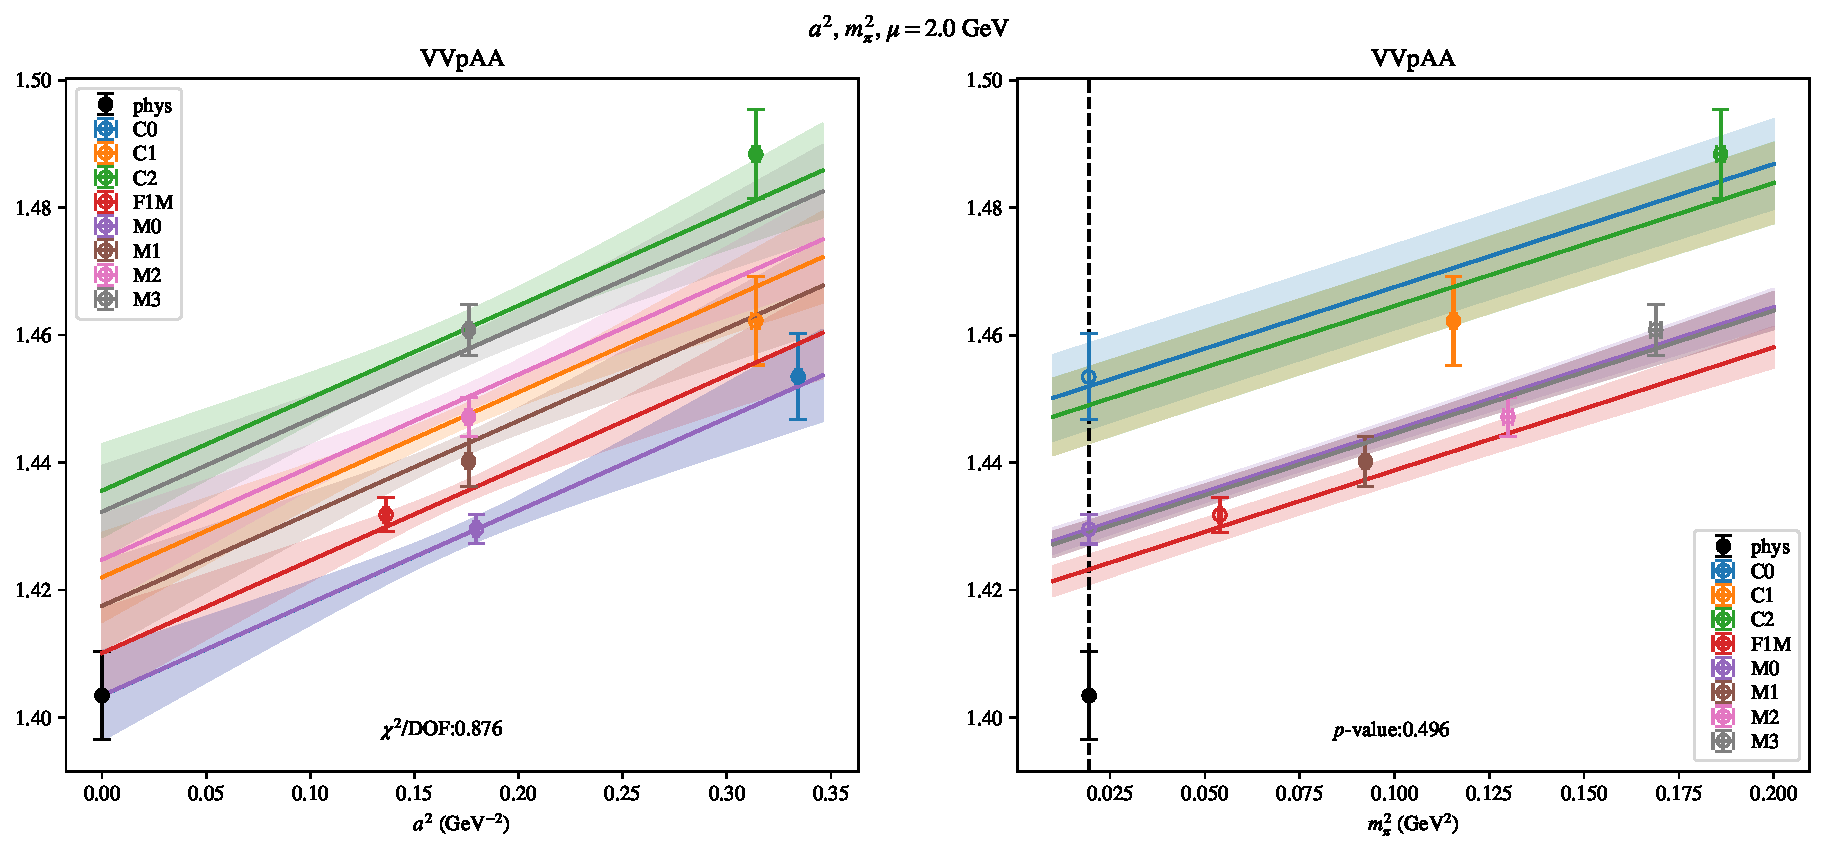
\includepdf[link, pages=-]{VVpAA/NPR/a2m2_20.pdf}
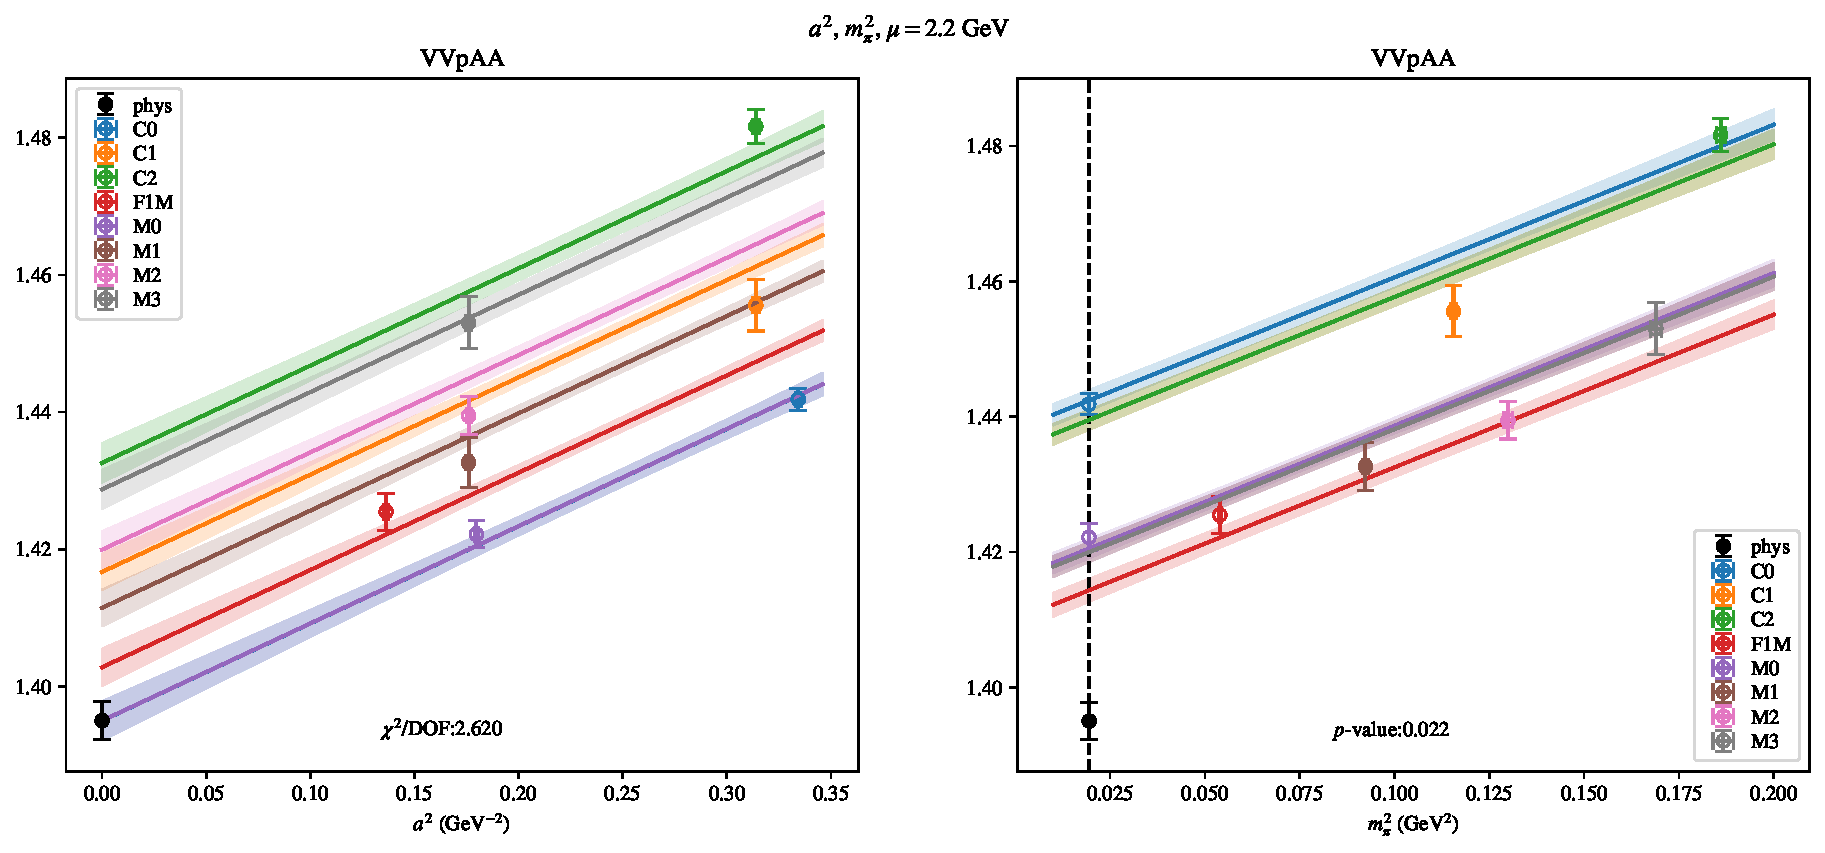
\includepdf[link, pages=-]{VVpAA/NPR/a2m2_22.pdf}
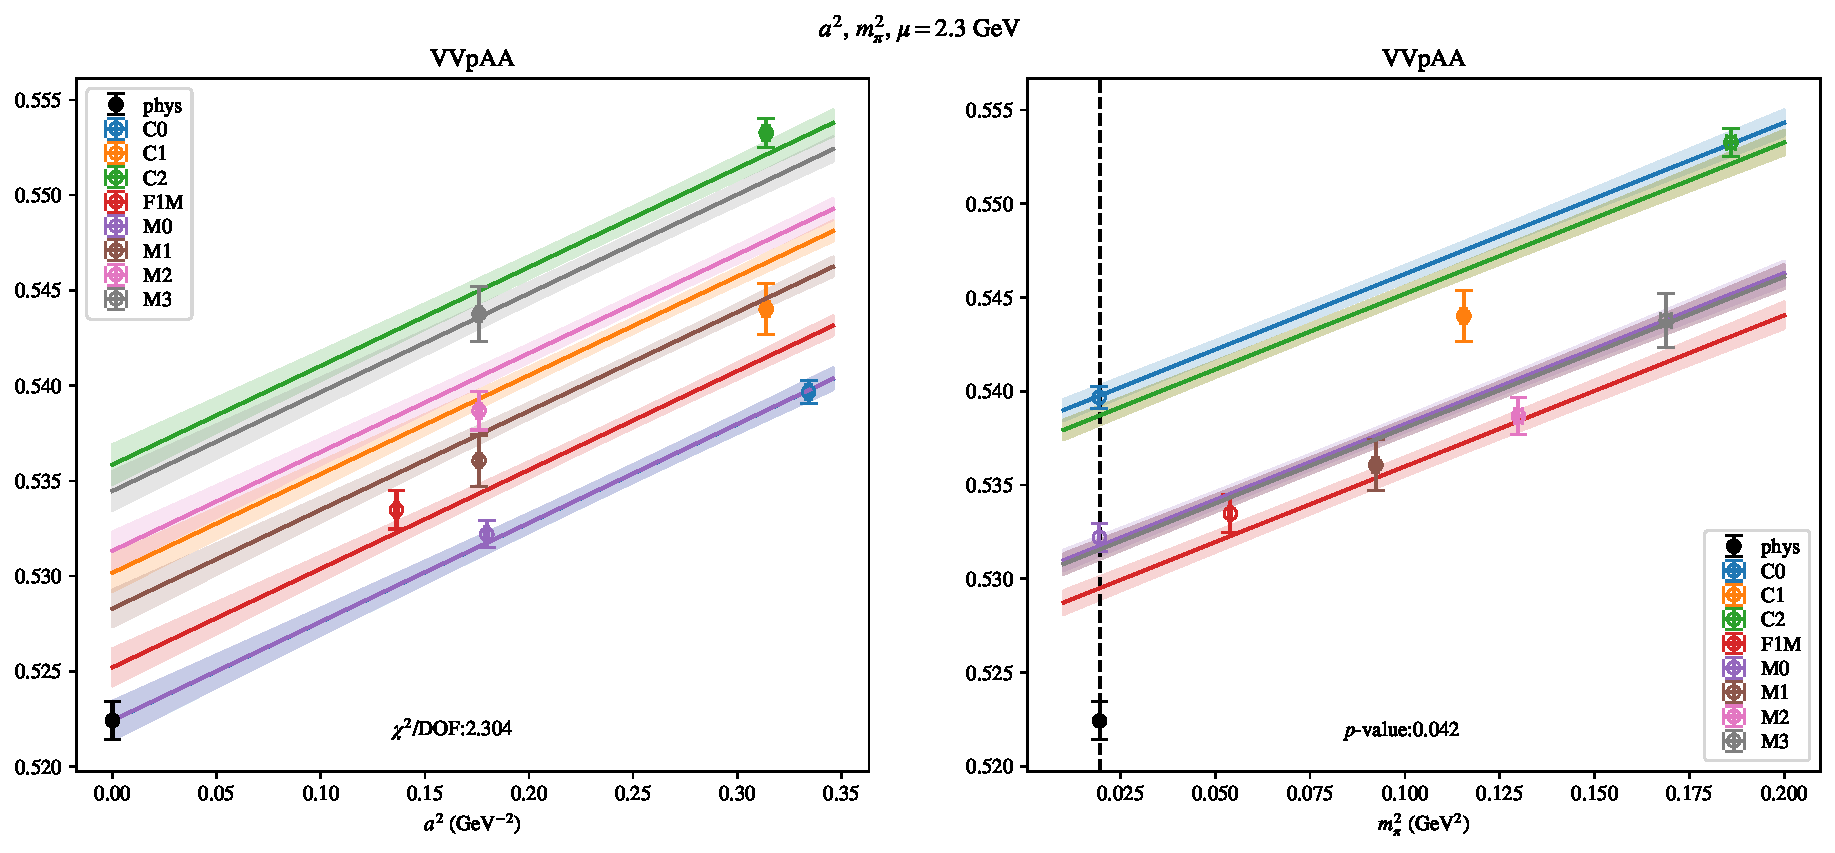
\includepdf[link, pages=-]{VVpAA/NPR/a2m2_23.pdf}
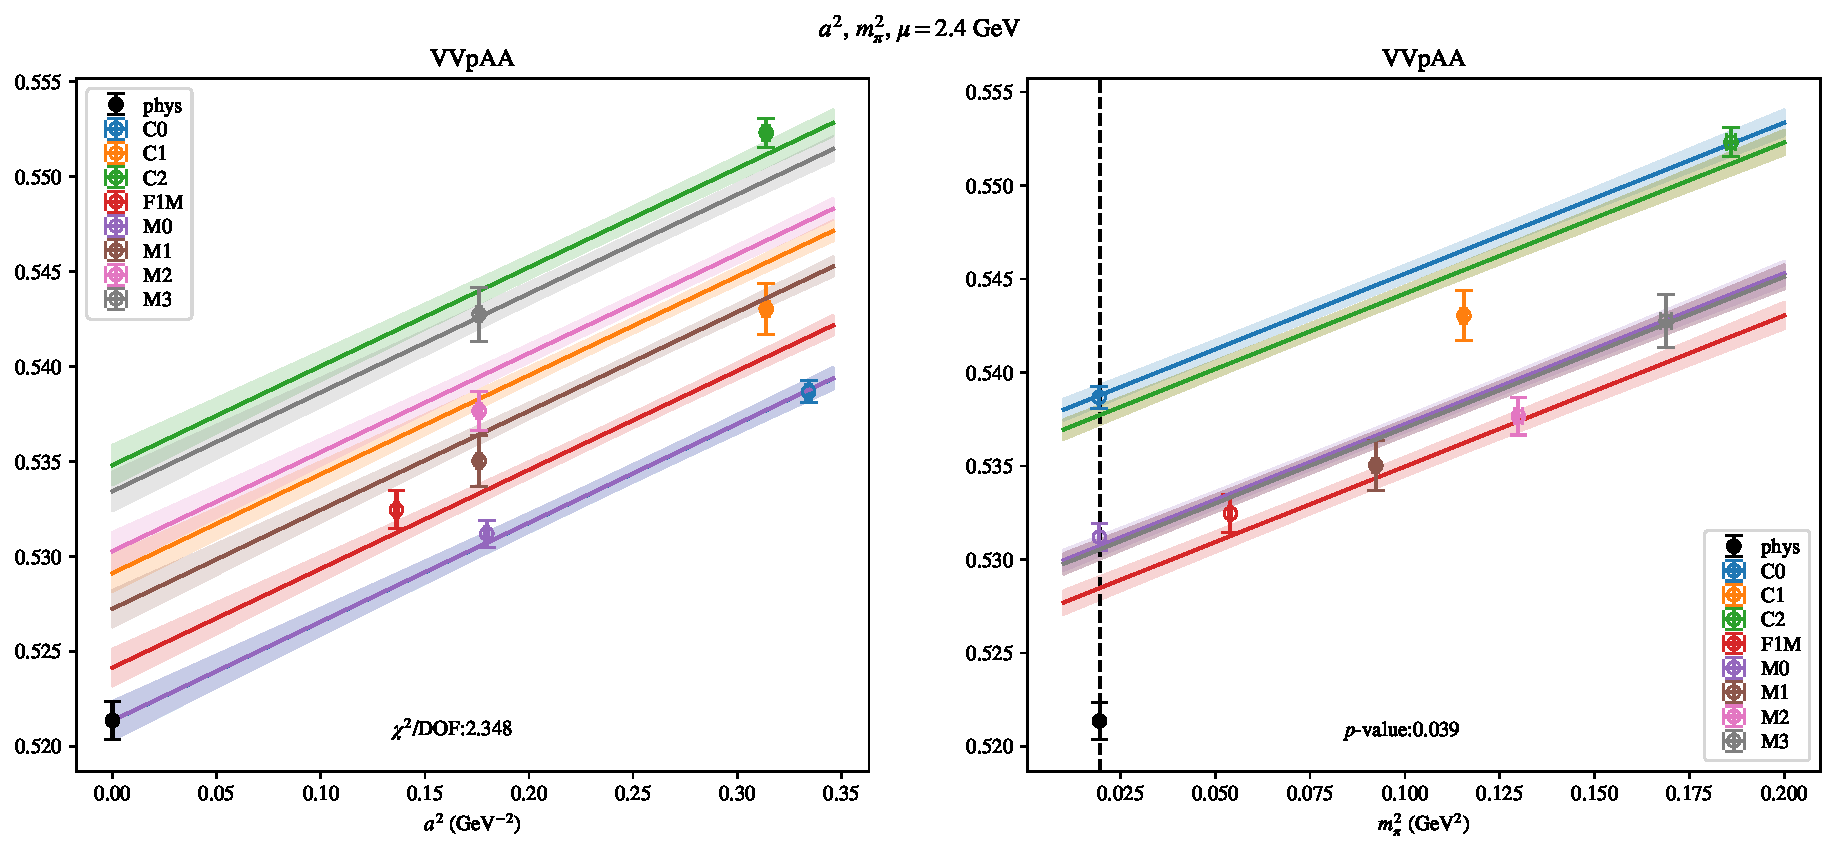
\includepdf[link, pages=-]{VVpAA/NPR/a2m2_24.pdf}
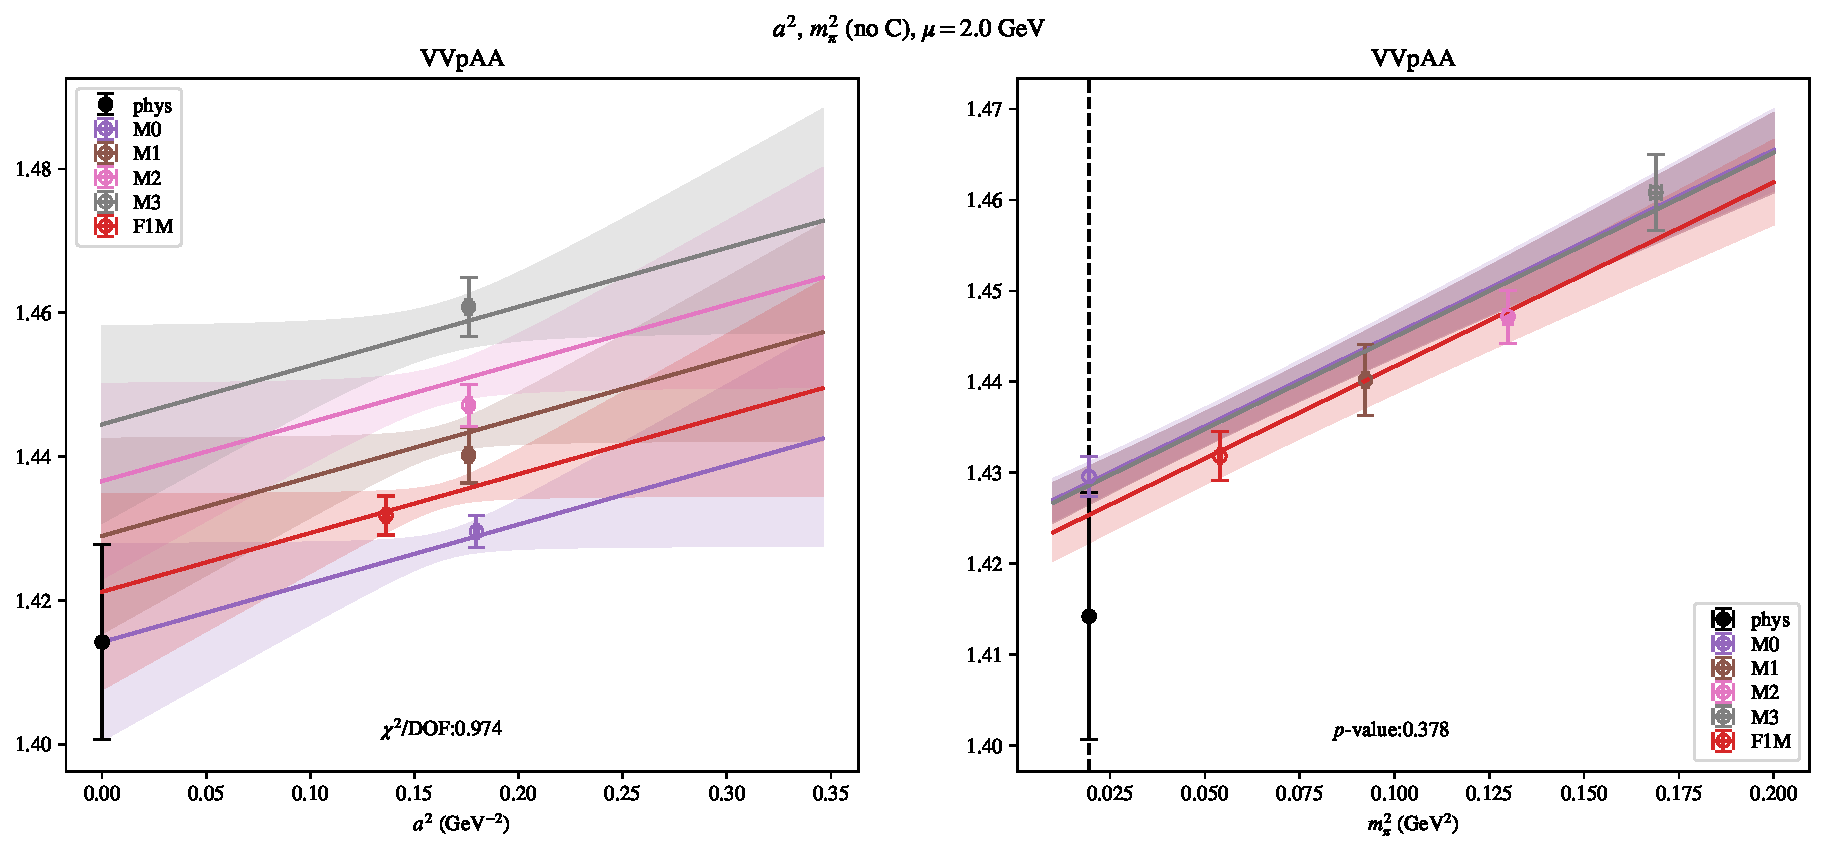
\includepdf[link, pages=-]{VVpAA/NPR/a2m2noC_20.pdf}
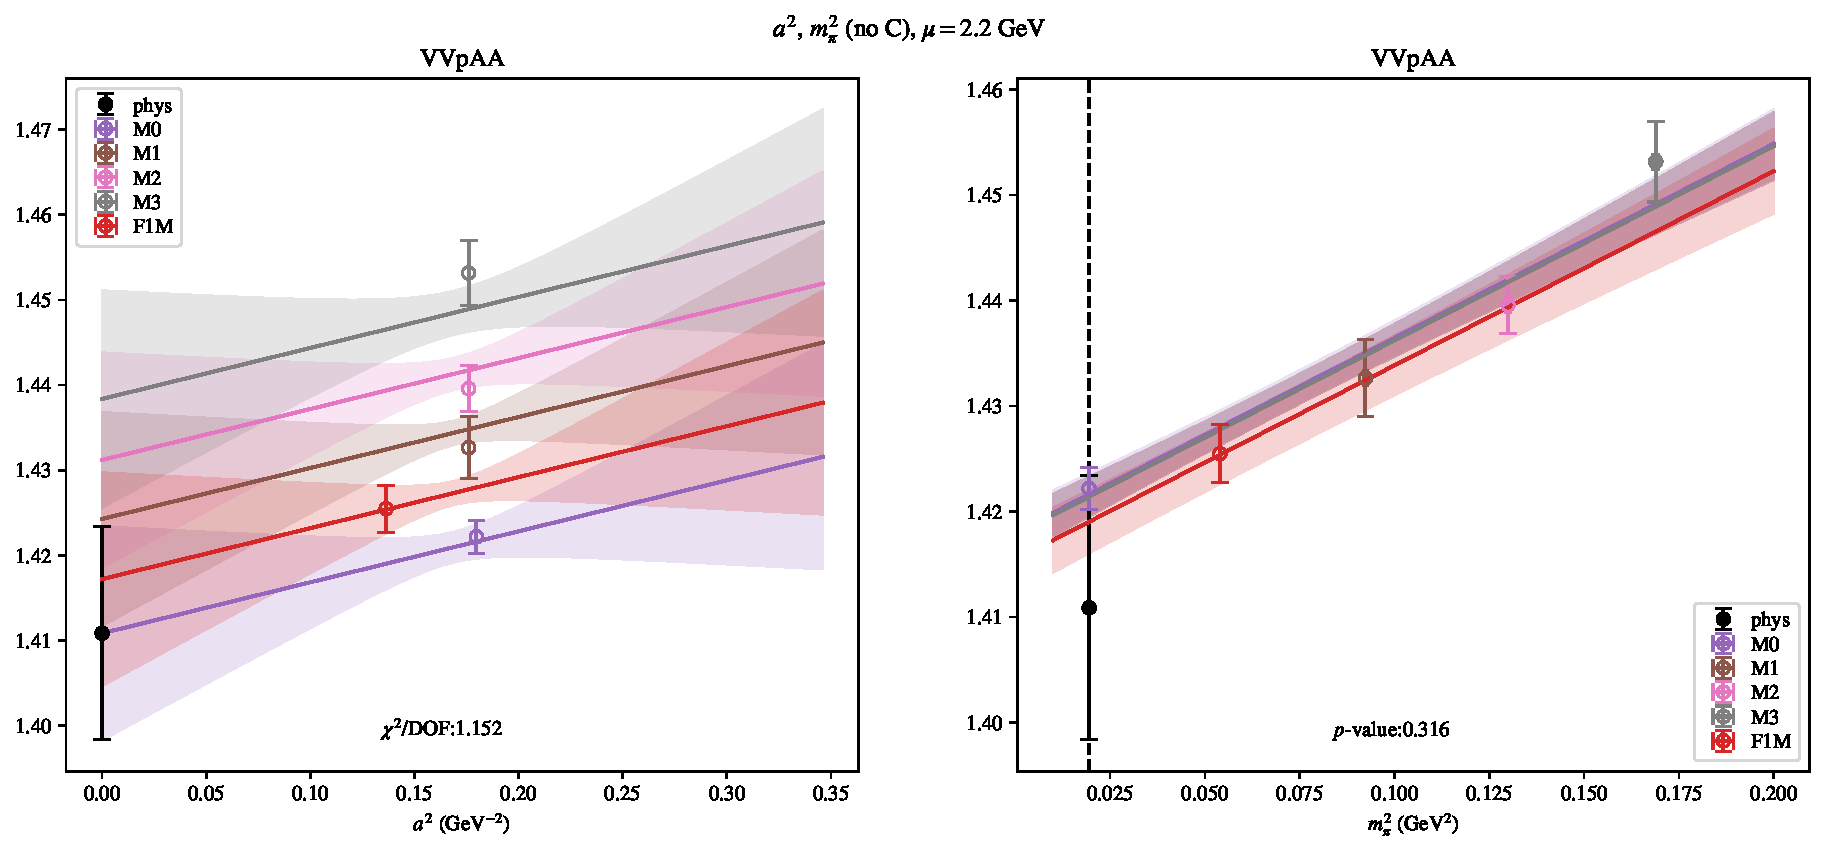
\includepdf[link, pages=-]{VVpAA/NPR/a2m2noC_22.pdf}
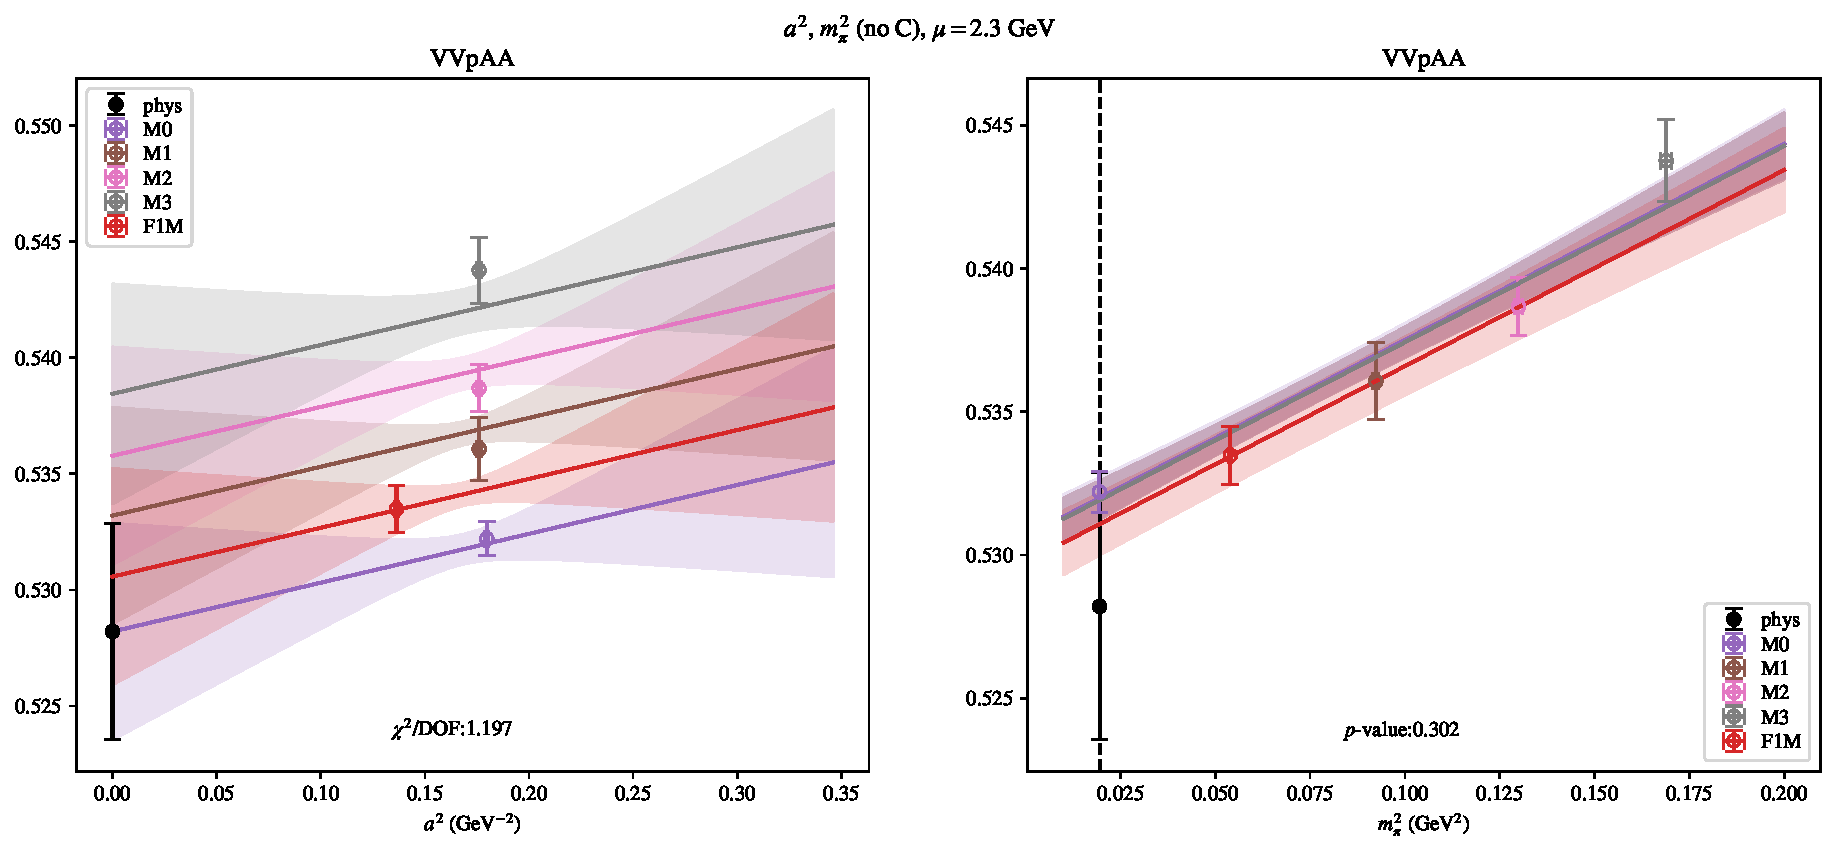
\includepdf[link, pages=-]{VVpAA/NPR/a2m2noC_23.pdf}
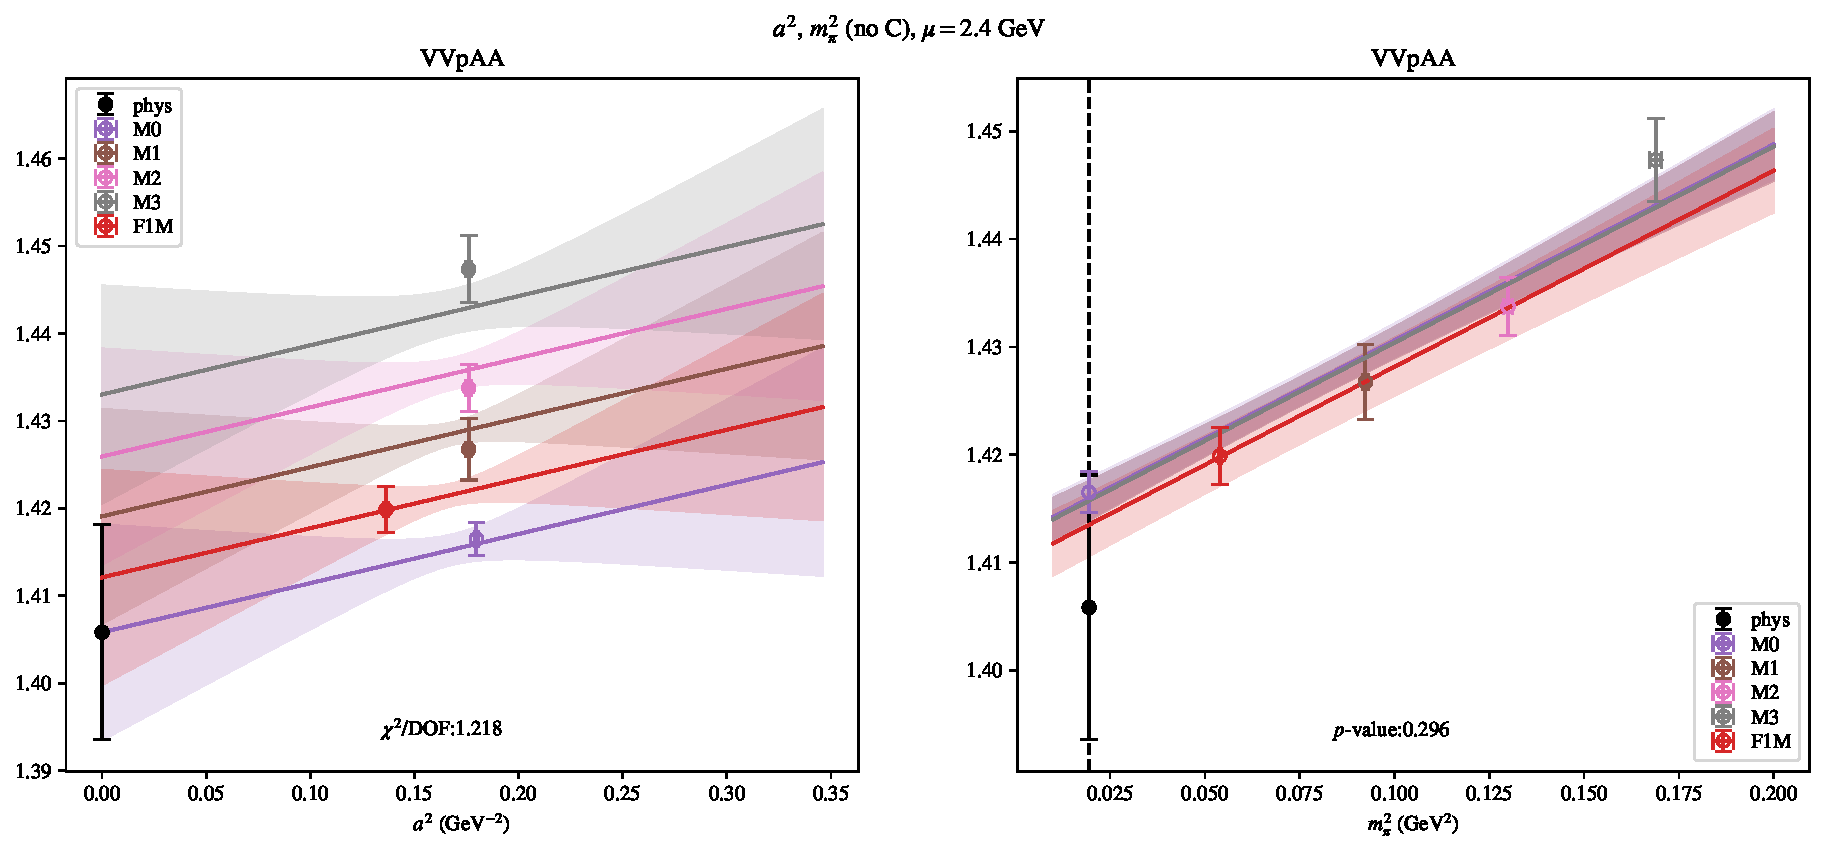
\includepdf[link, pages=-]{VVpAA/NPR/a2m2noC_24.pdf}
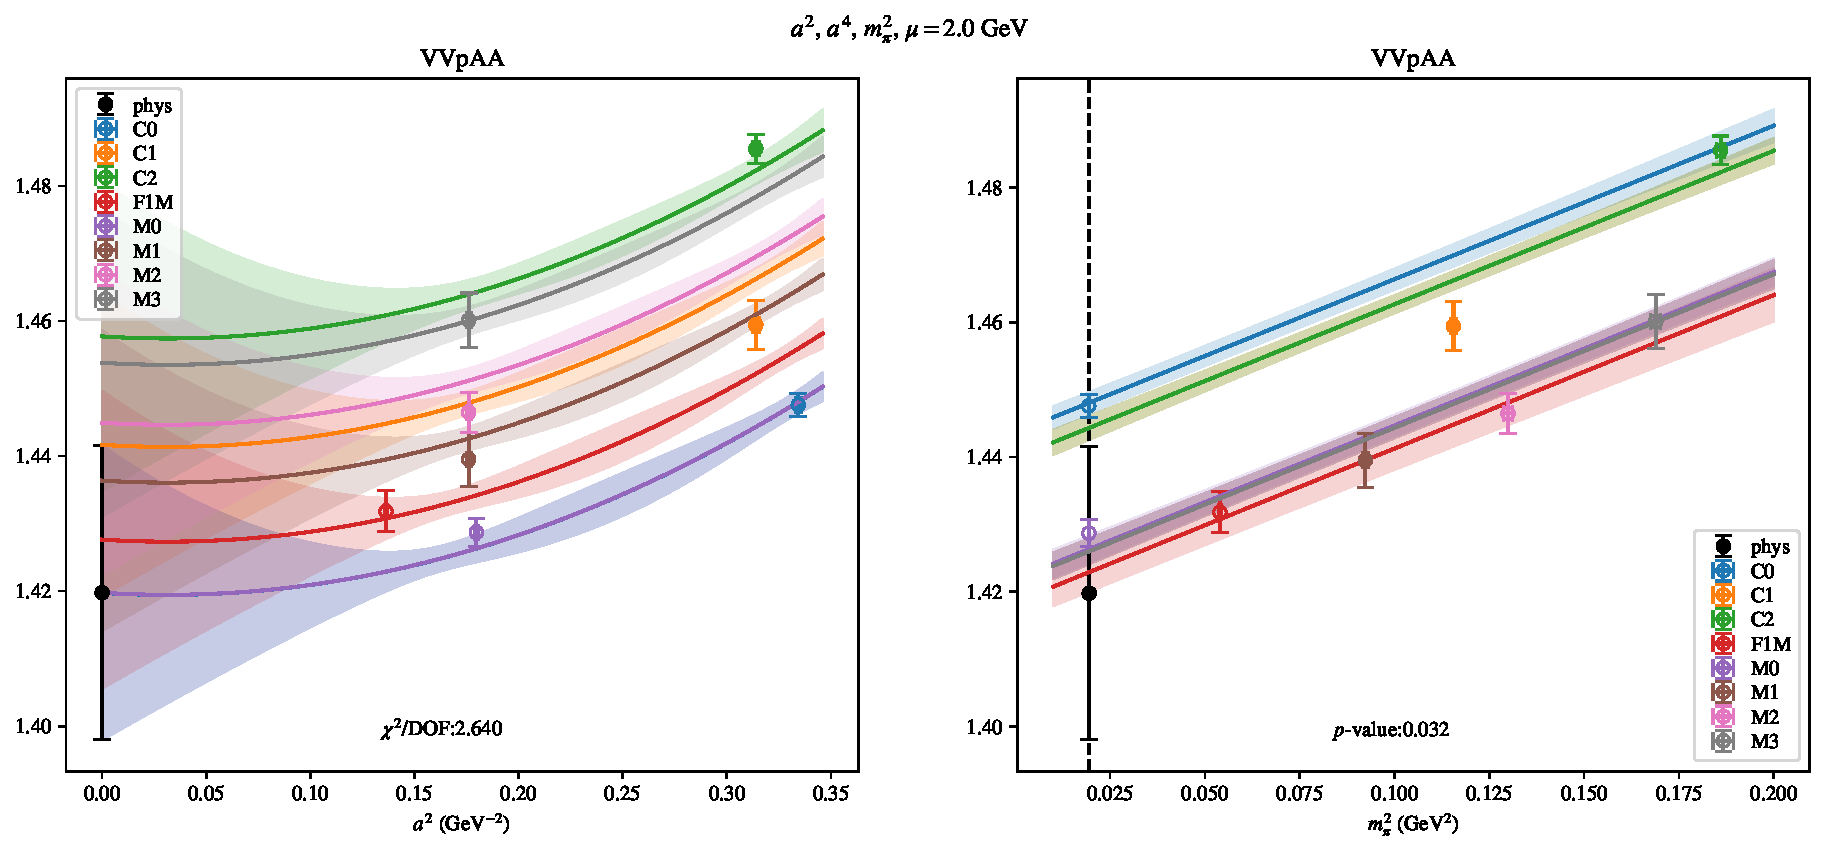
\includepdf[link, pages=-]{VVpAA/NPR/a2a4m2_20.pdf}
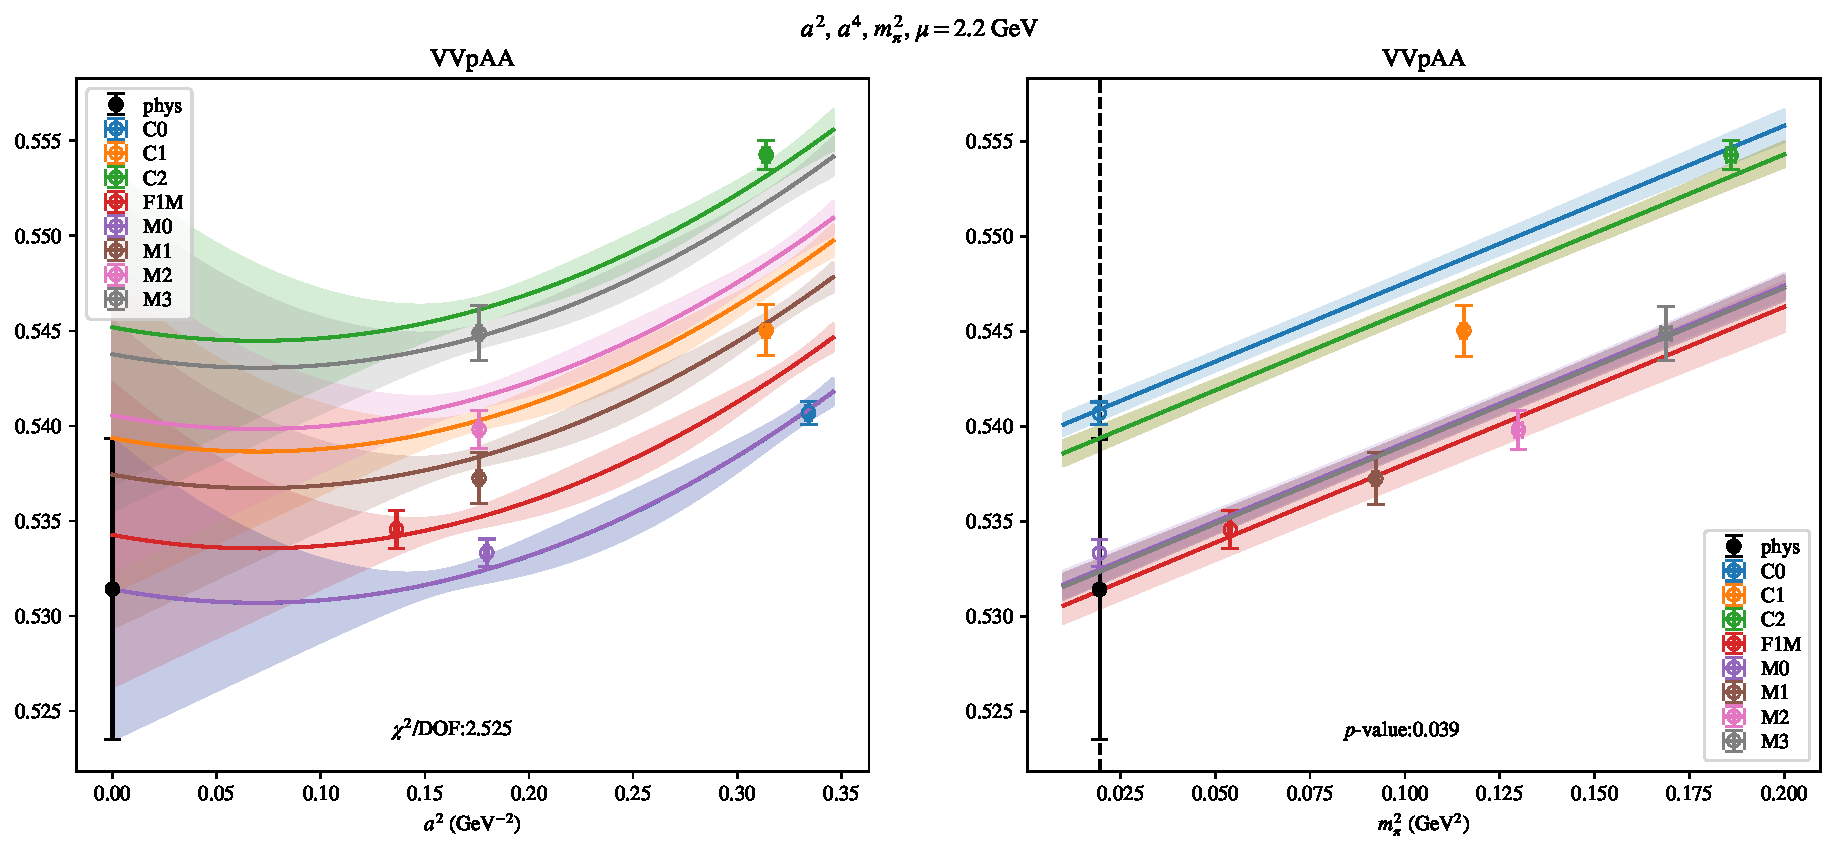
\includepdf[link, pages=-]{VVpAA/NPR/a2a4m2_22.pdf}
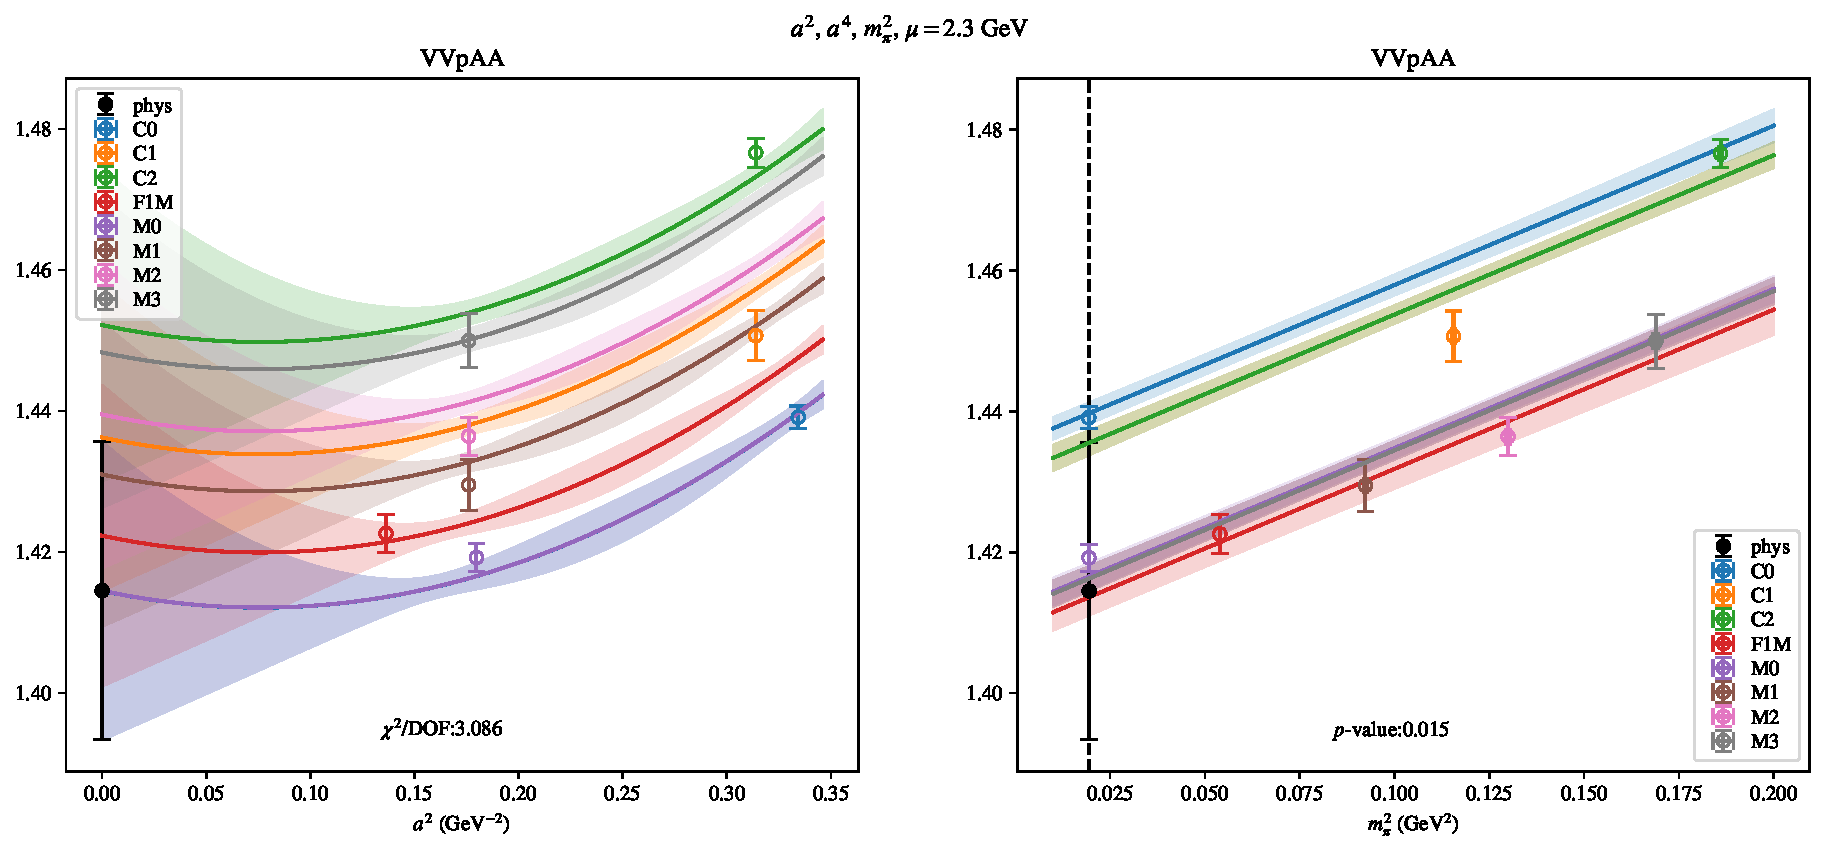
\includepdf[link, pages=-]{VVpAA/NPR/a2a4m2_23.pdf}
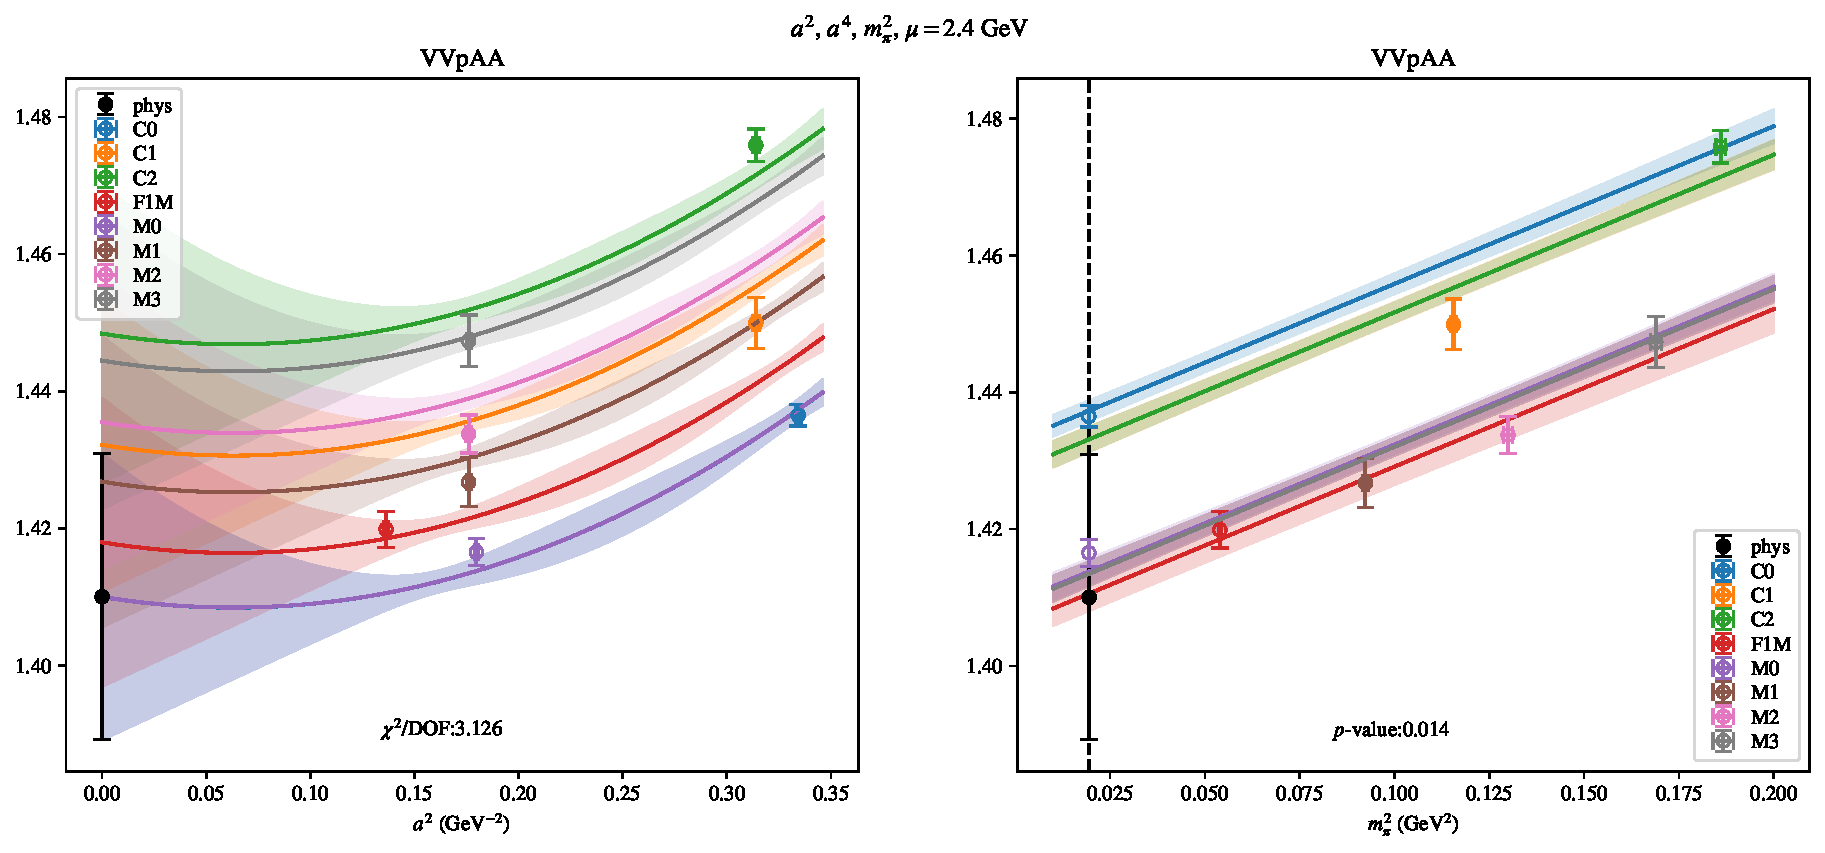
\includepdf[link, pages=-]{VVpAA/NPR/a2a4m2_24.pdf}
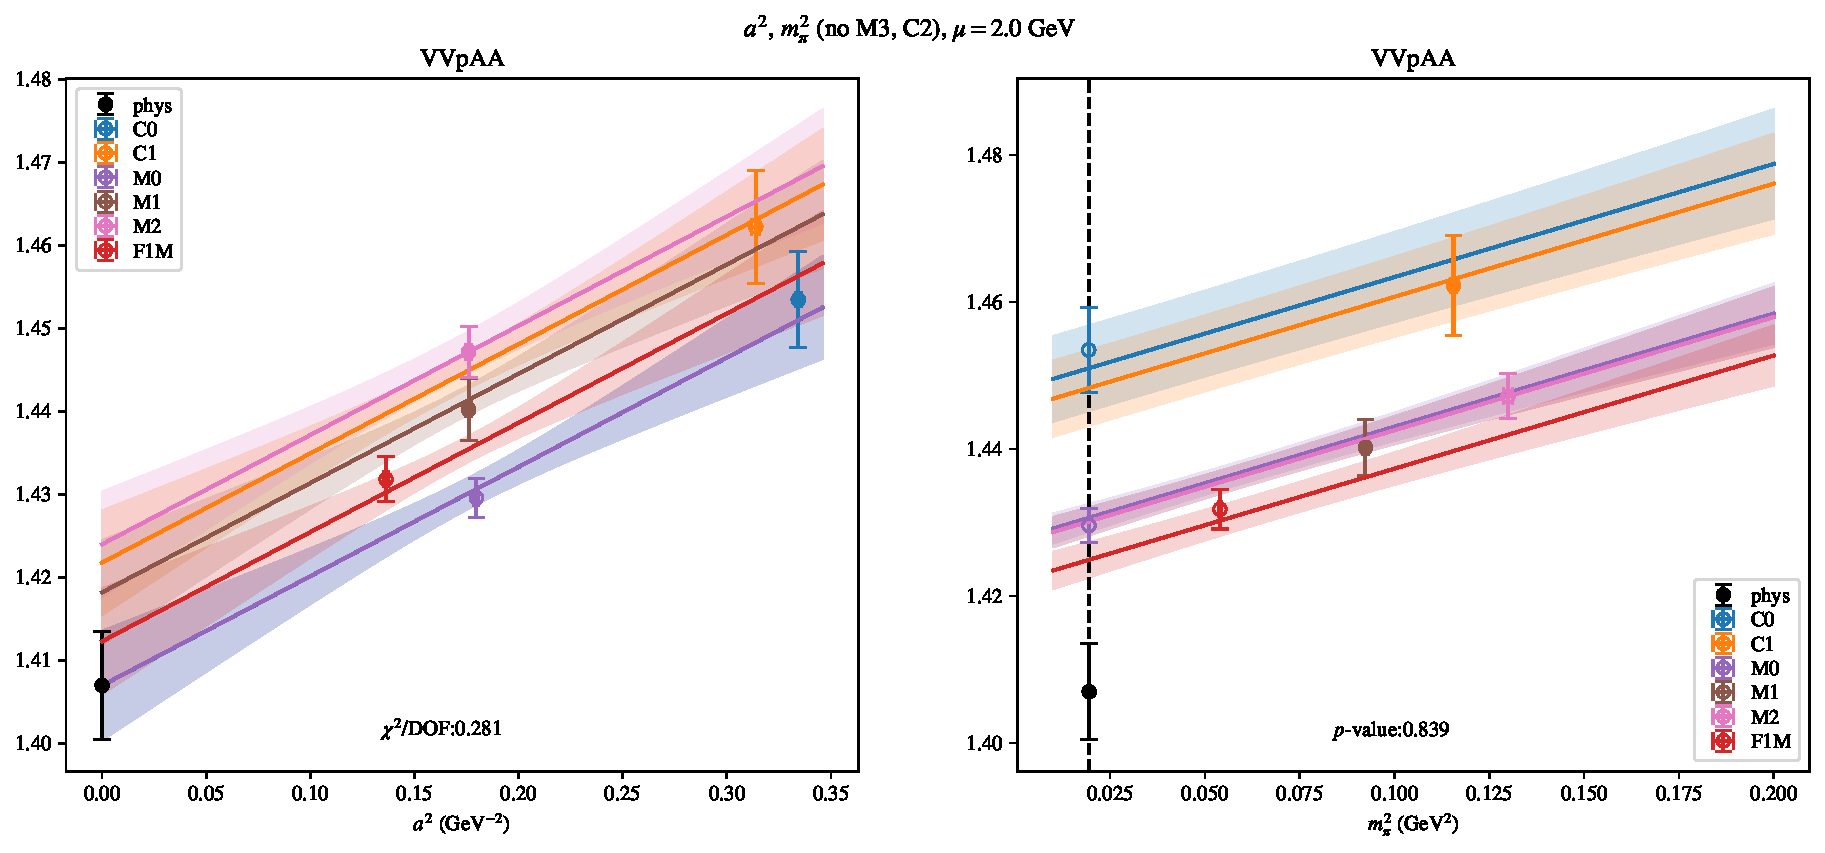
\includepdf[link, pages=-]{VVpAA/NPR/a2m2mcut_20.pdf}
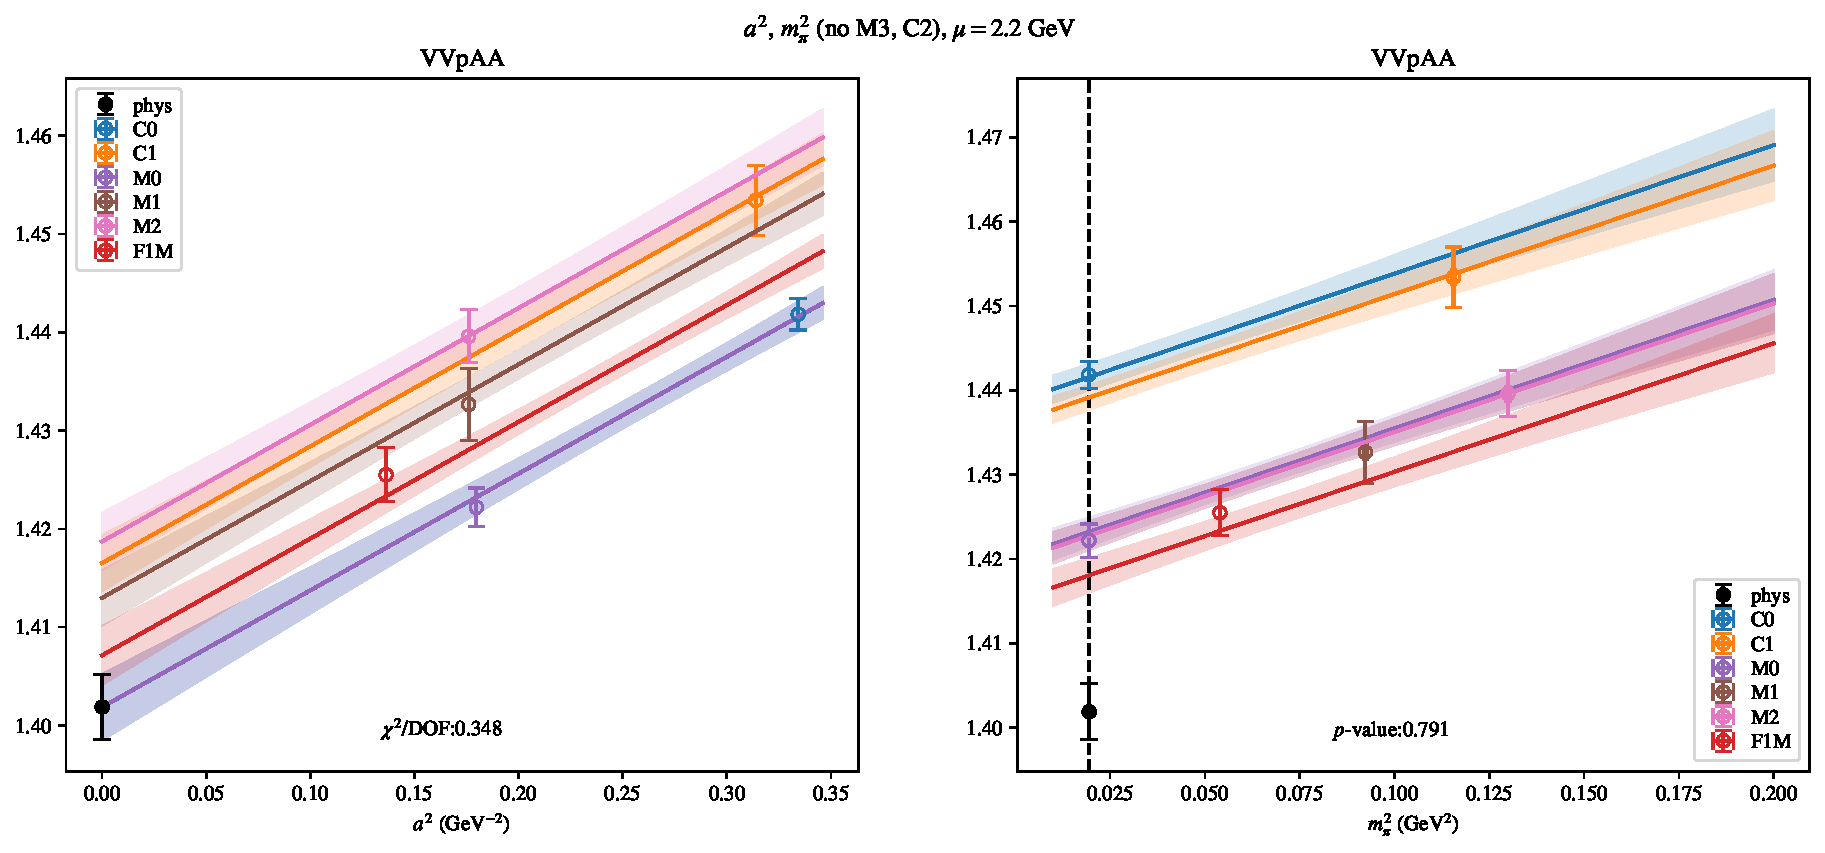
\includepdf[link, pages=-]{VVpAA/NPR/a2m2mcut_22.pdf}
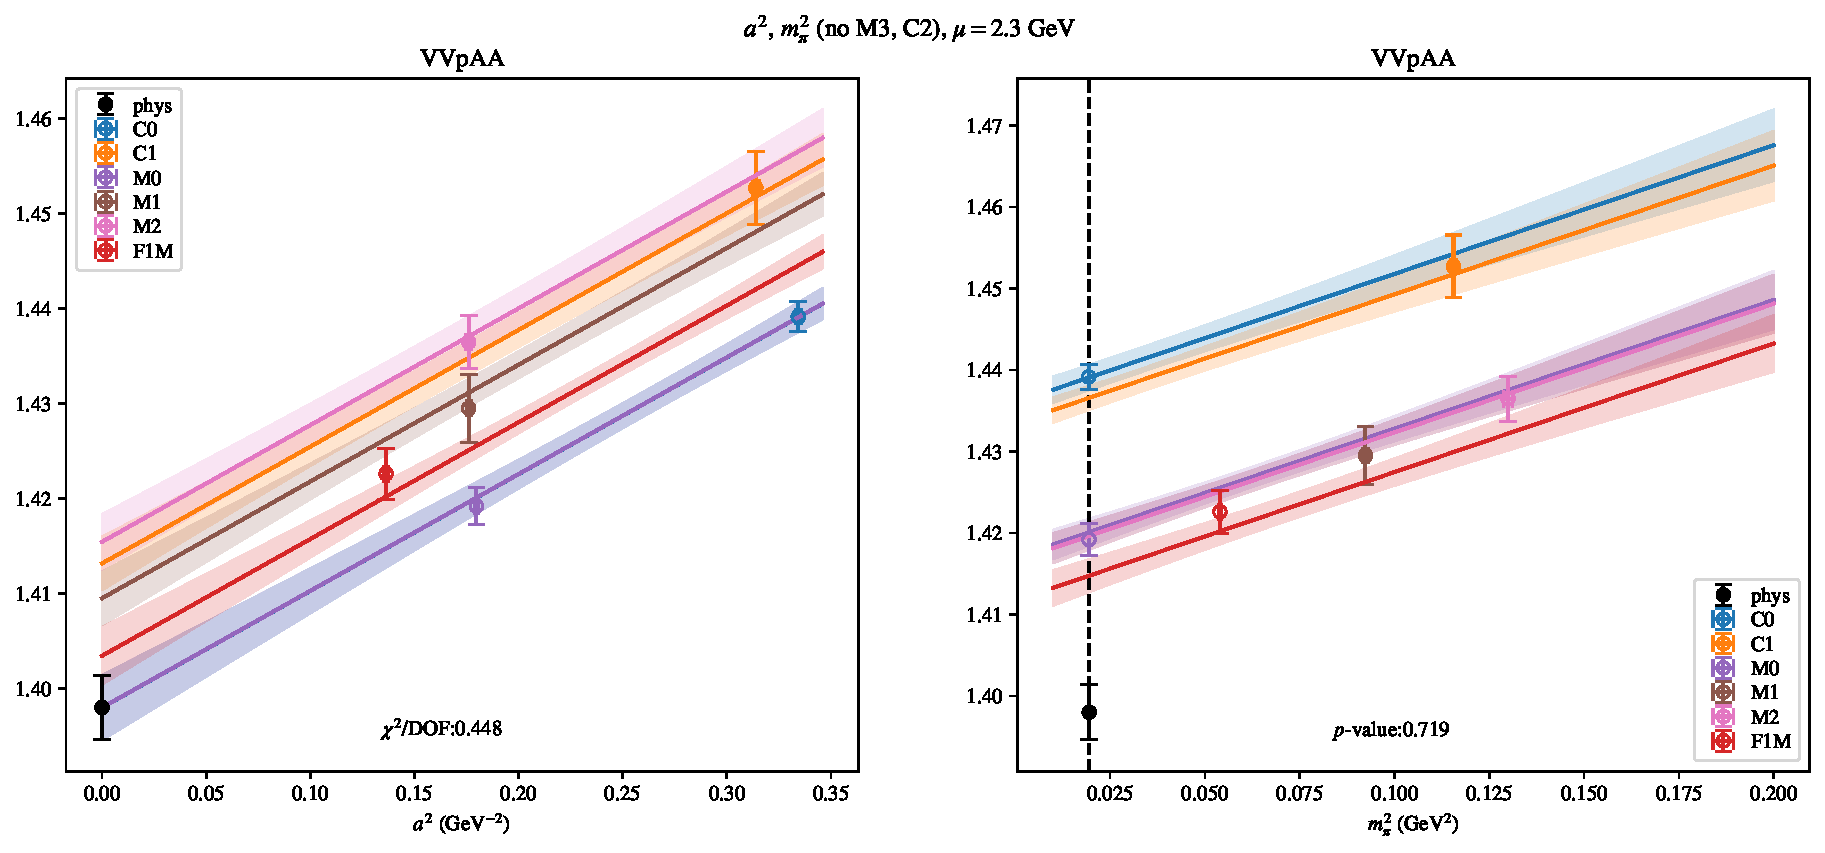
\includepdf[link, pages=-]{VVpAA/NPR/a2m2mcut_23.pdf}
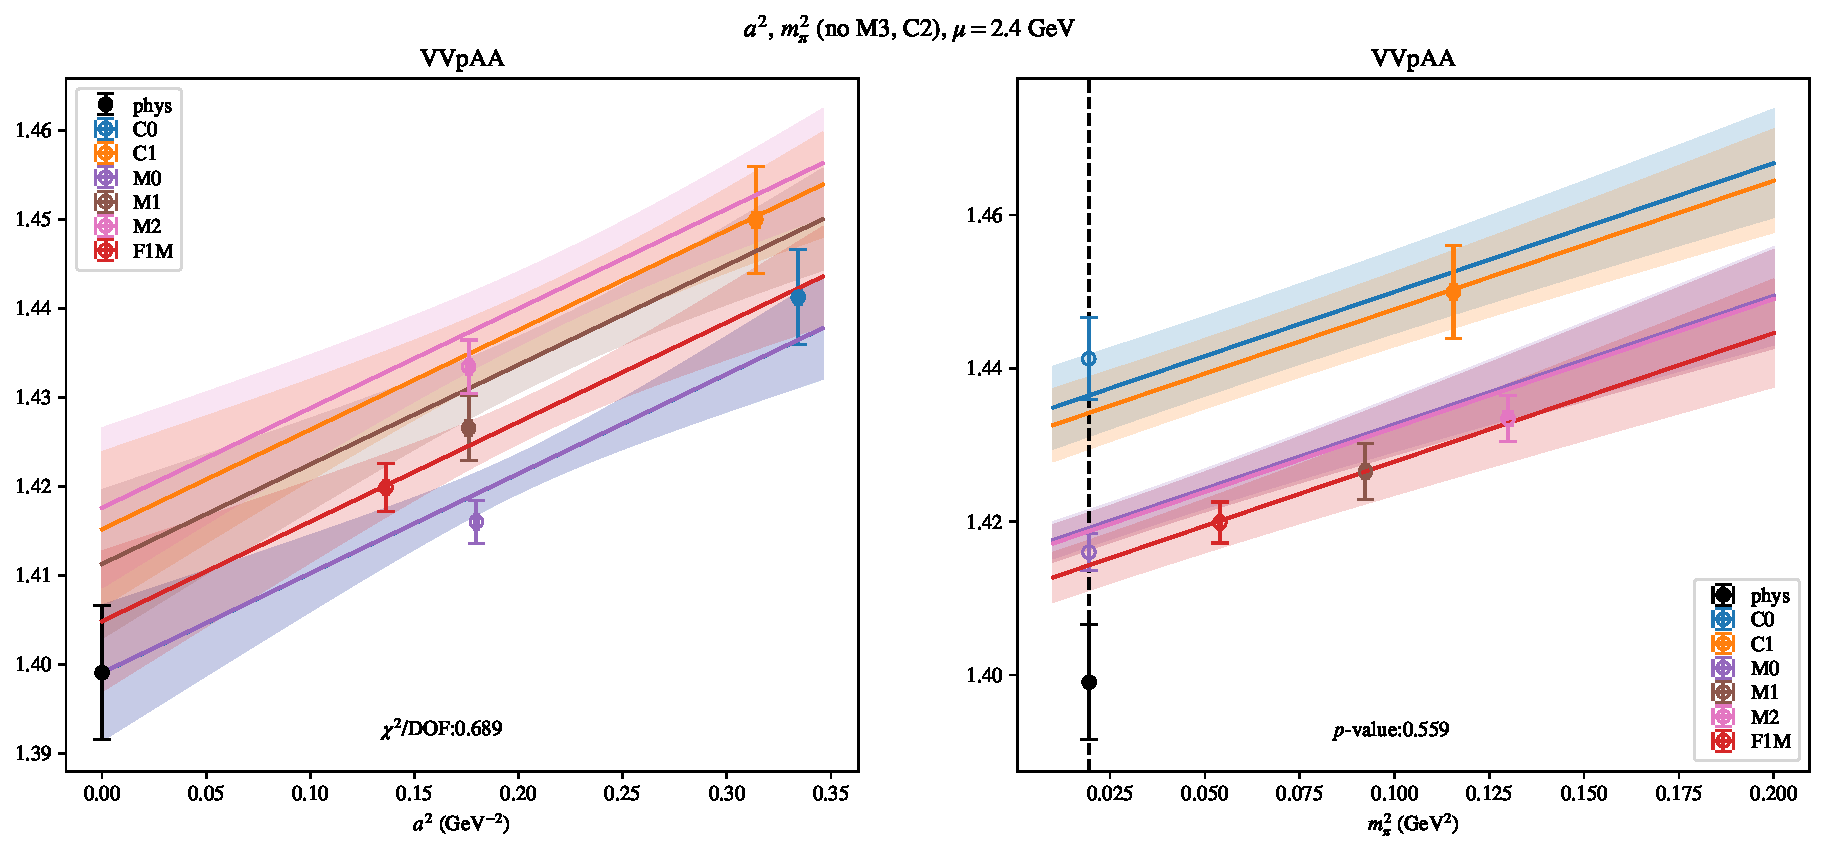
\includepdf[link, pages=-]{VVpAA/NPR/a2m2mcut_24.pdf}
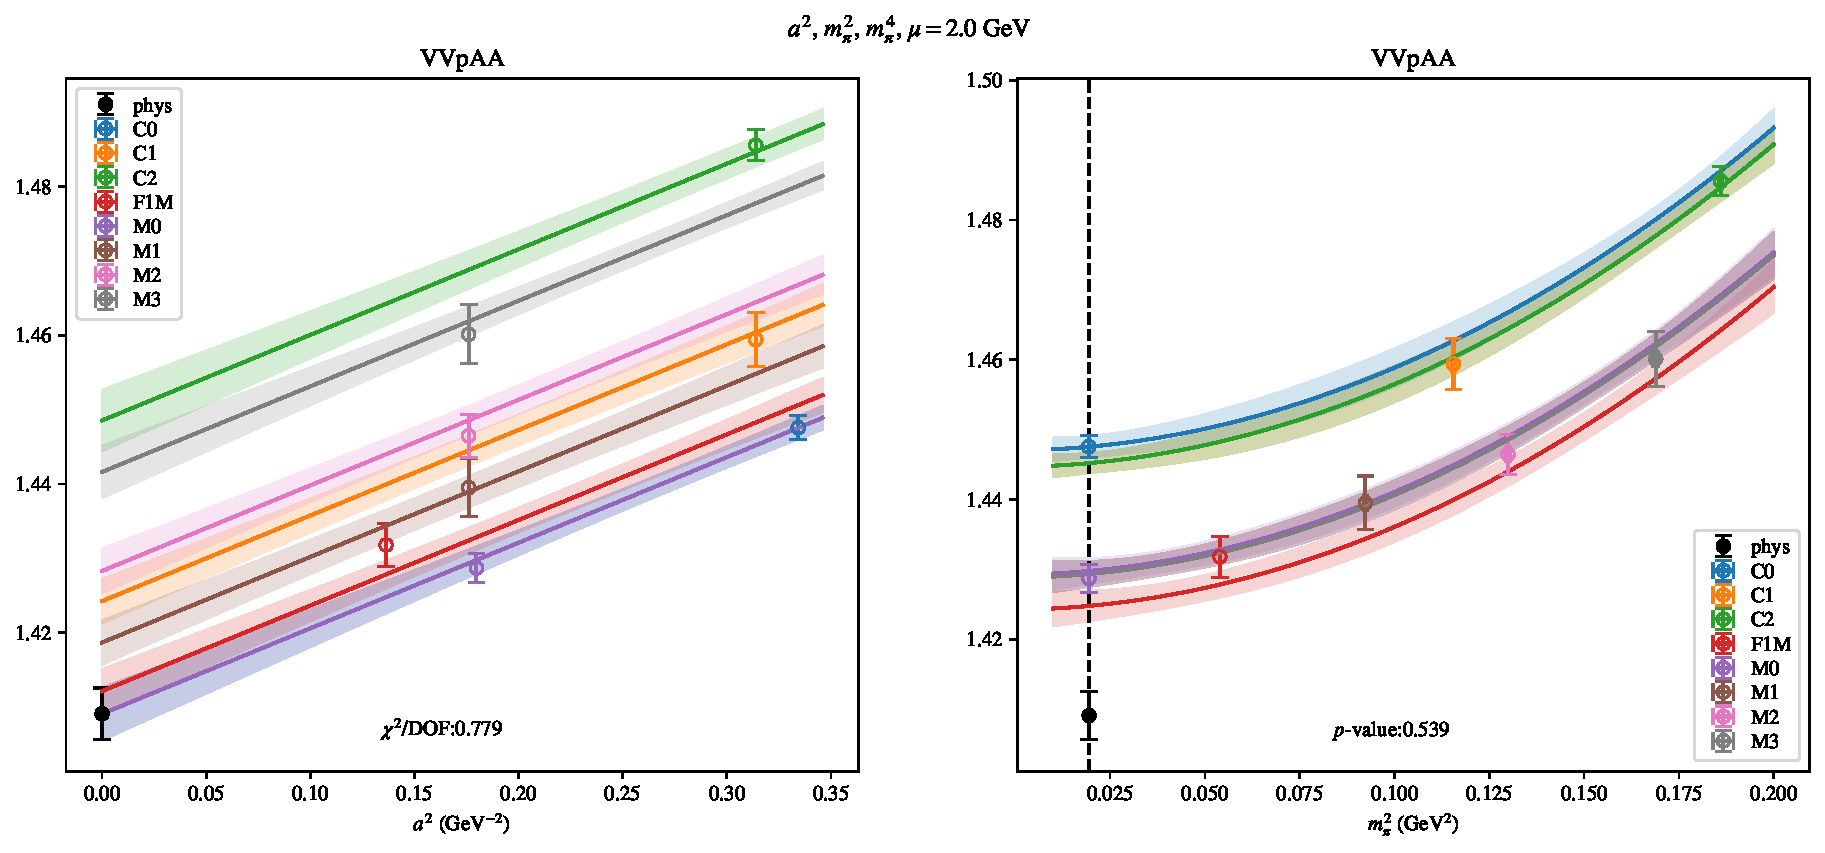
\includepdf[link, pages=-]{VVpAA/NPR/a2m2m4_20.pdf}
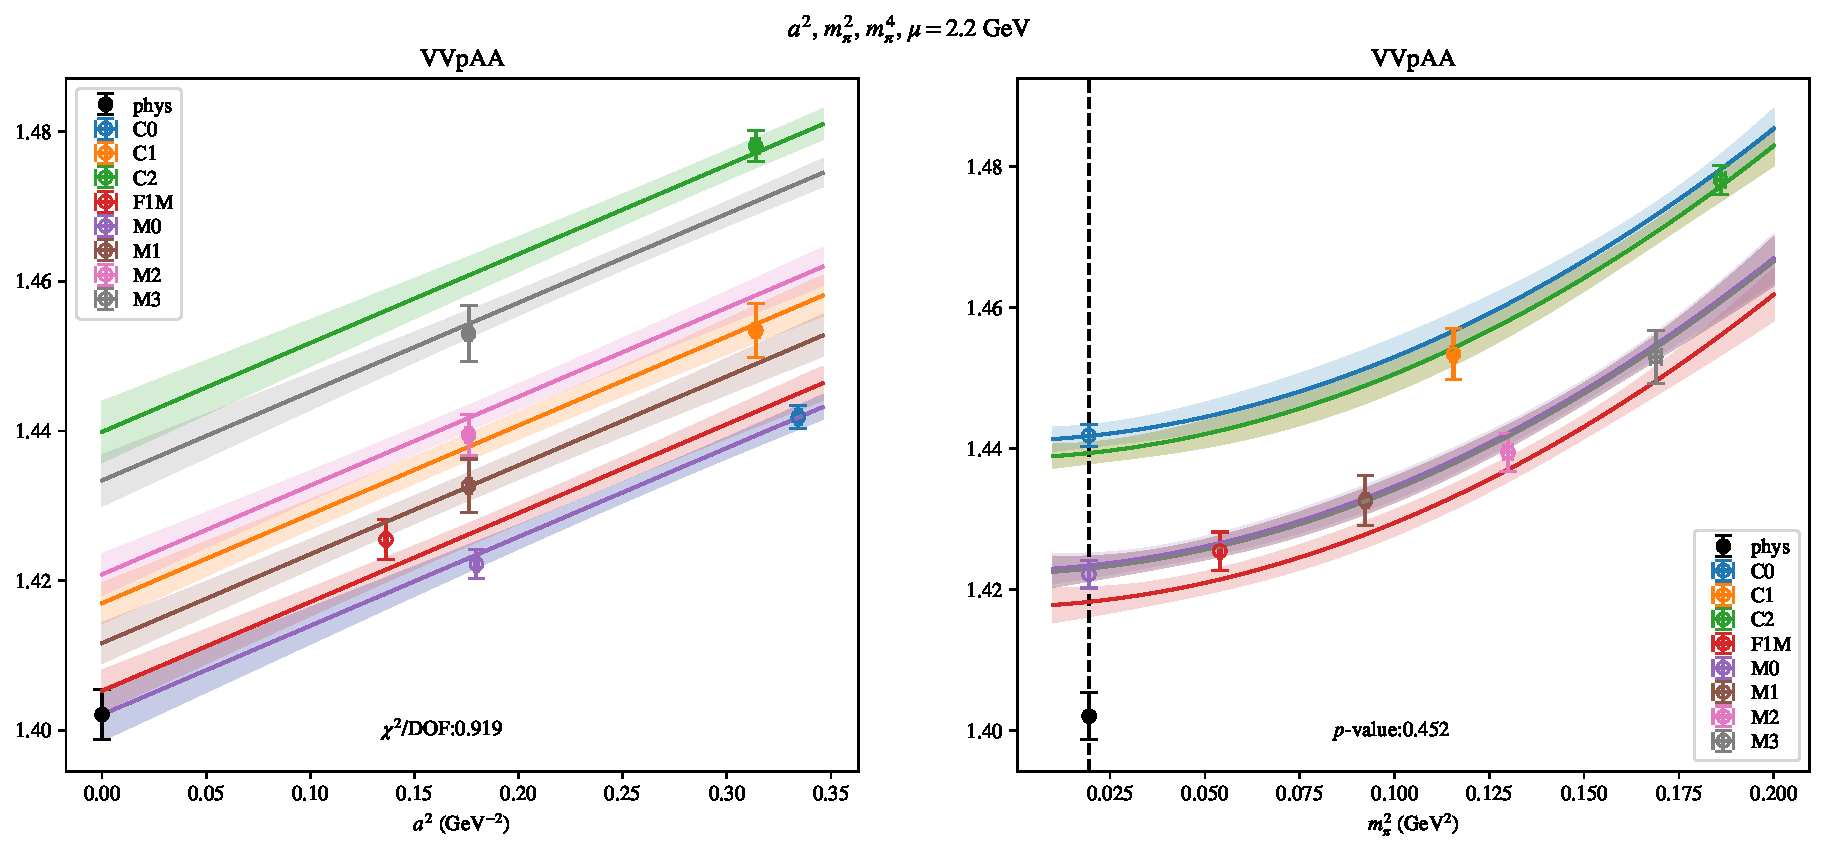
\includepdf[link, pages=-]{VVpAA/NPR/a2m2m4_22.pdf}
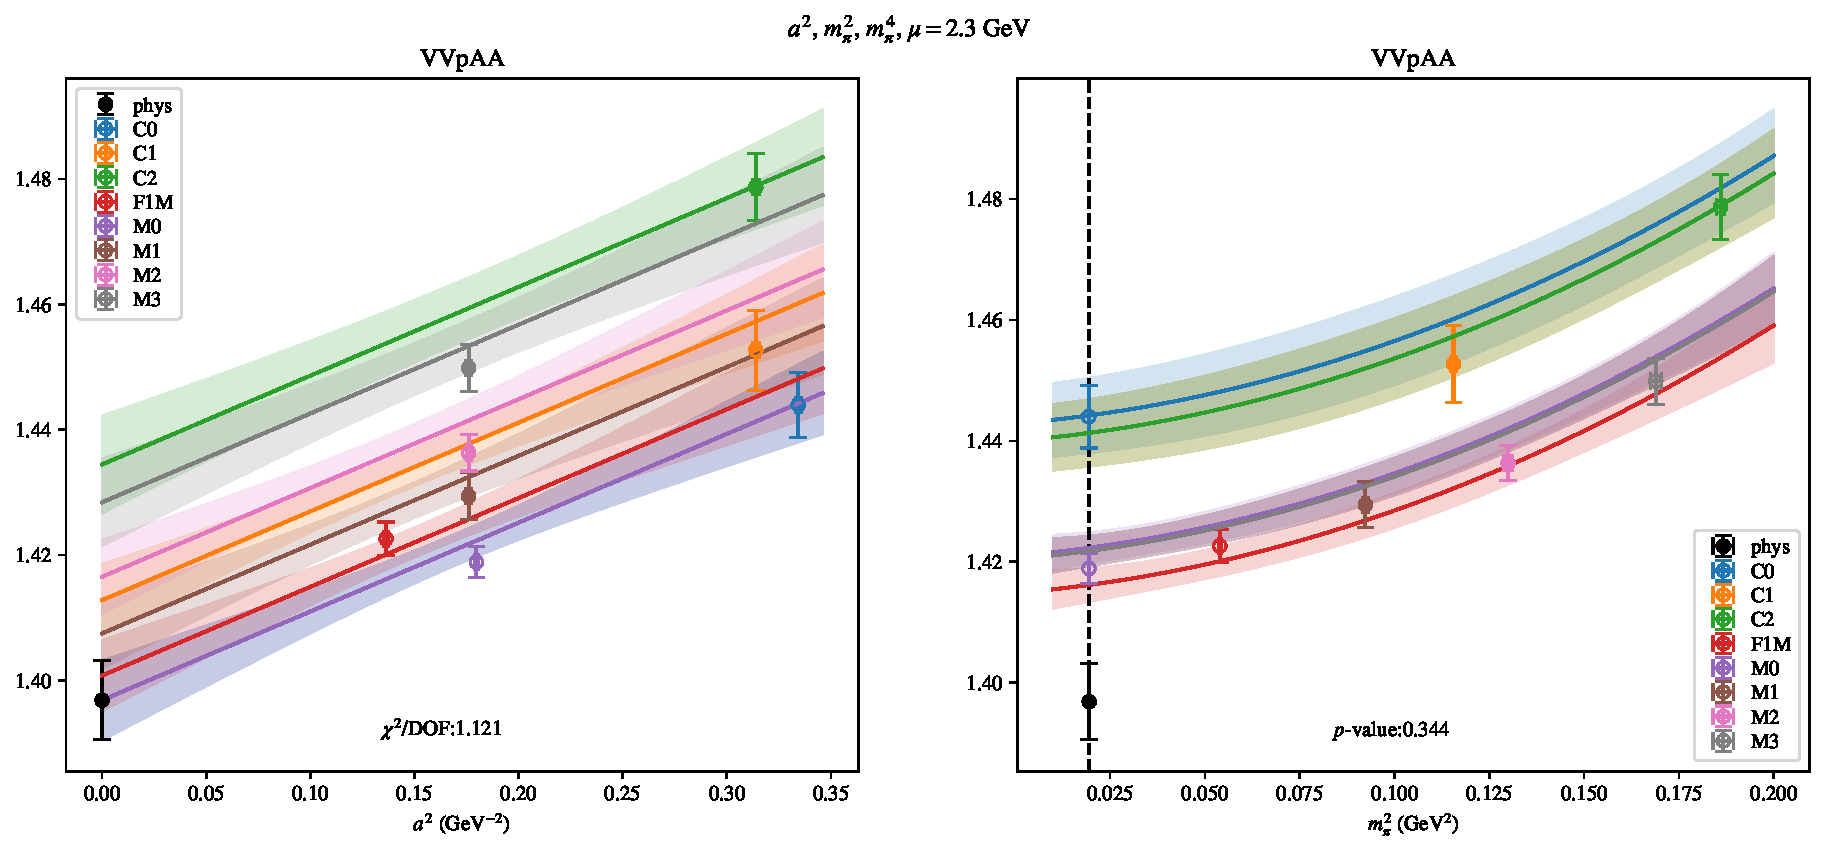
\includepdf[link, pages=-]{VVpAA/NPR/a2m2m4_23.pdf}
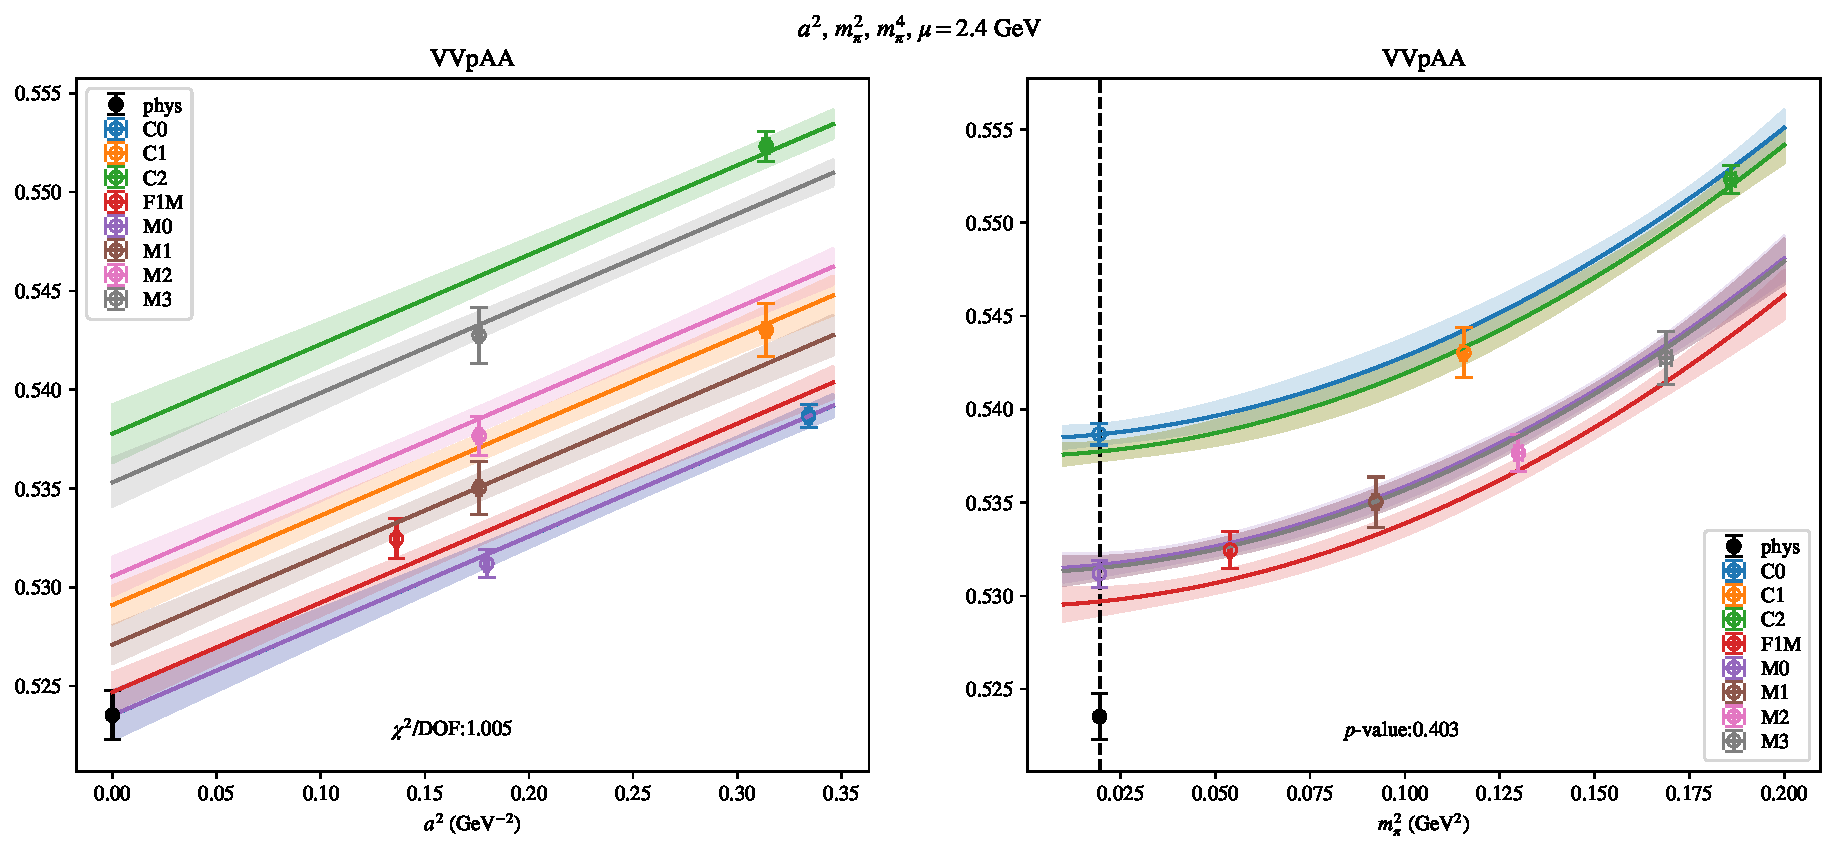
\includepdf[link, pages=-]{VVpAA/NPR/a2m2m4_24.pdf}
\clearpage
\section{$\mathcal{B}_2$}
\begin{table}[h!]
\begin{center}
\begin{tabular}{|c|c|c|c|c|c|}
\hline
$\mu$ (GeV) & $a^2$, $m_\pi^2$& $a^2$, $m_\pi^2$ (no C)& $a^2$, $a^4$, $m_\pi^2$& $a^2$, $m_\pi^2$ (no M3, C2)& $a^2$, $m_\pi^2$, $m_\pi^4$\\
\hline
2.0& \hyperlink{VVmAA/NPR/a2m2_20.pdf.1}{\textbf{-1.012(14)}: 3.704 (0.002)} & \hyperlink{VVmAA/NPR/a2m2noC_20.pdf.1}{\textbf{-0.985(89)}: 3.202 (0.041)} & \hyperlink{VVmAA/NPR/a2a4m2_20.pdf.1}{\textbf{-0.96(13)}: 1.718 (0.143)} & \hyperlink{VVmAA/NPR/a2m2mcut_20.pdf.1}{\textbf{-1.013(14)}: 4.797 (0.002)} & \hyperlink{VVmAA/NPR/a2m2m4_20.pdf.1}{\textbf{-1.014(14)}: 2.798 (0.024)}\\
2.2& \hyperlink{VVmAA/NPR/a2m2_22.pdf.1}{\textbf{-1.019(13)}: 4.377 (0.001)} & \hyperlink{VVmAA/NPR/a2m2noC_22.pdf.1}{\textbf{-0.988(87)}: 3.605 (0.027)} & \hyperlink{VVmAA/NPR/a2a4m2_22.pdf.1}{\textbf{-0.96(13)}: 2.066 (0.082)} & \hyperlink{VVmAA/NPR/a2m2mcut_22.pdf.1}{\textbf{-1.020(14)}: 5.498 (0.001)} & \hyperlink{VVmAA/NPR/a2m2m4_22.pdf.1}{\textbf{-1.021(14)}: 3.222 (0.012)}\\
2.3& \hyperlink{VVmAA/NPR/a2m2_23.pdf.1}{\textbf{-1.022(13)}: 4.739 (0.0)} & \hyperlink{VVmAA/NPR/a2m2noC_23.pdf.1}{\textbf{-0.989(86)}: 3.604 (0.027)} & \hyperlink{VVmAA/NPR/a2a4m2_23.pdf.1}{\textbf{-0.97(12)}: 2.182 (0.068)} & \hyperlink{VVmAA/NPR/a2m2mcut_23.pdf.1}{\textbf{-1.023(14)}: 5.979 (0.0)} & \hyperlink{VVmAA/NPR/a2m2m4_23.pdf.1}{\textbf{-1.024(14)}: 3.542 (0.007)}\\
2.4& \hyperlink{VVmAA/NPR/a2m2_24.pdf.1}{\textbf{-1.025(13)}: 4.969 (0.0)} & \hyperlink{VVmAA/NPR/a2m2noC_24.pdf.1}{\textbf{-0.991(85)}: 3.686 (0.025)} & \hyperlink{VVmAA/NPR/a2a4m2_24.pdf.1}{\textbf{-0.97(12)}: 2.337 (0.053)} & \hyperlink{VVmAA/NPR/a2m2mcut_24.pdf.1}{\textbf{-1.026(14)}: 6.196 (0.0)} & \hyperlink{VVmAA/NPR/a2m2m4_24.pdf.1}{\textbf{-1.027(14)}: 3.669 (0.005)}\\
\hline
\end{tabular}
\caption{Physical point value from chiral and continuum extrapolation at renormalisation scale $\mu$. Entries are \textbf{value(error)}: $\chi^2/\text{DOF}$ ($p$-value).}
\end{center}
\end{table}
\begin{table}[h!]
\begin{center}
\begin{tabular}{|c c|c|c|c|c|c|}
\hline
$\mu$ (GeV) &  & $a^2$, $m_\pi^2$& $a^2$, $m_\pi^2$ (no C)& $a^2$, $a^4$, $m_\pi^2$& $a^2$, $m_\pi^2$ (no M3, C2)& $a^2$, $m_\pi^2$, $m_\pi^4$\\
\hline
\multirow{2}{0.5in}{2.0} & $\alpha$ & -0.177(49)& -0.01(51)& 0.26(12)& -0.179(50)& -0.181(50)\\
 & $\beta$ & 0.00192(11)& 0.00179(20)& 0.00186(12)& 0.00156(21)& 0.00019(64)\\
\hline
\multirow{2}{0.5in}{2.2} & $\alpha$ & -0.222(46)& -0.04(49)& 0.22(12)& -0.223(48)& -0.227(49)\\
 & $\beta$ & 0.00164(11)& 0.00160(19)& 0.00157(12)& 0.00127(20)& -0.0001(62)\\
\hline
\multirow{2}{0.5in}{2.3} & $\alpha$ & -0.245(46)& -0.06(48)& 0.21(12)& -0.246(48)& -0.250(48)\\
 & $\beta$ & 0.00154(11)& 0.00153(19)& 0.00145(12)& 0.00116(20)& -0.0003(61)\\
\hline
\multirow{2}{0.5in}{2.4} & $\alpha$ & -0.266(45)& -0.07(48)& 0.20(12)& -0.267(47)& -0.271(47)\\
 & $\beta$ & 0.00144(11)& 0.00143(19)& 0.00134(11)& 0.00104(20)& -0.0004(61)\\
\hline
\end{tabular}
\caption{Fit values of coefficients in $Q = Q_{phys} + \mathbf{\alpha} a^2 + \mathbf{\beta}\left(\frac{m_\pi^2}{f_\pi^2}-\frac{m_{\pi,PDG}^2}{f_\pi^2}\right) + \ldots$.}
\end{center}
\end{table}
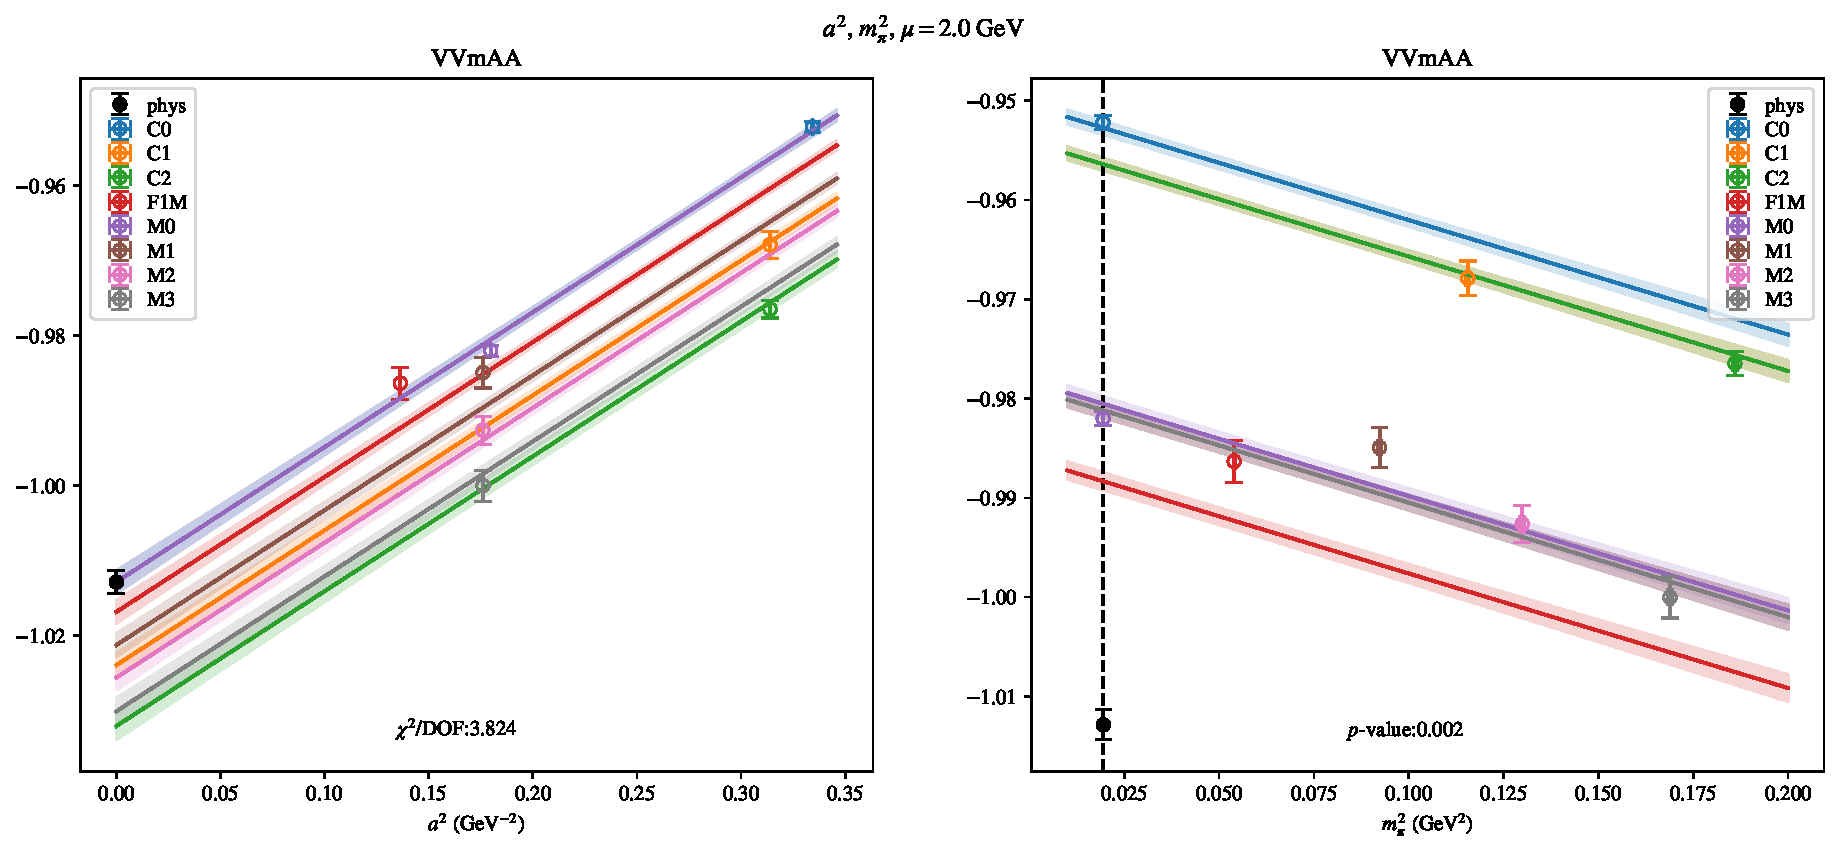
\includepdf[link, pages=-]{VVmAA/NPR/a2m2_20.pdf}
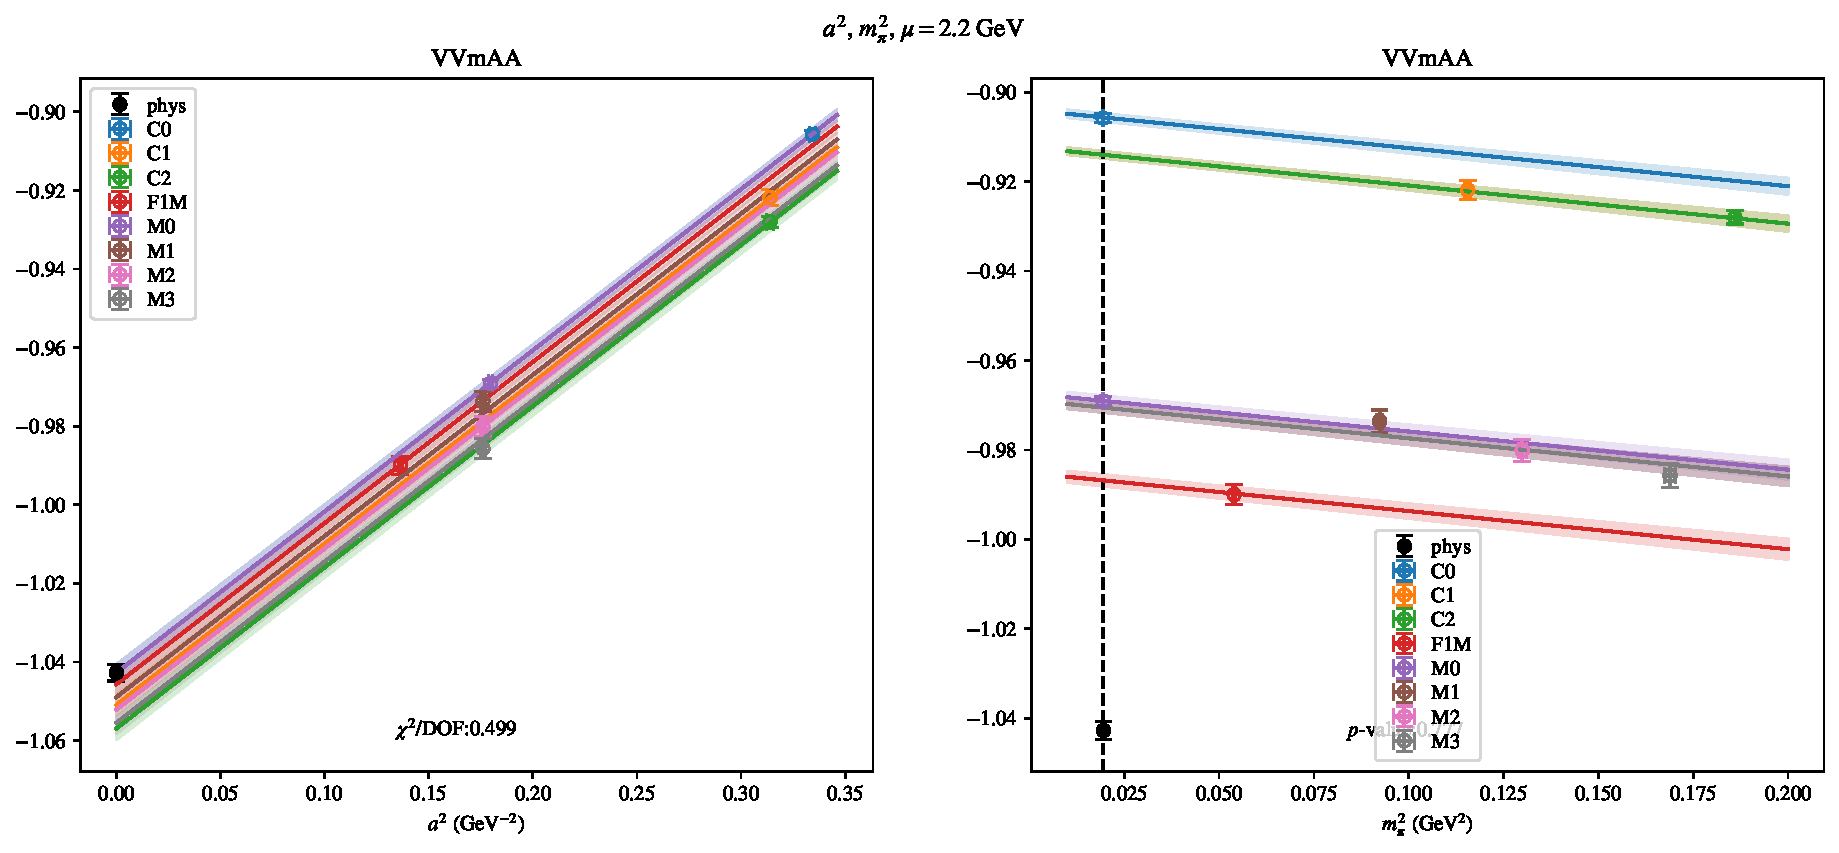
\includepdf[link, pages=-]{VVmAA/NPR/a2m2_22.pdf}
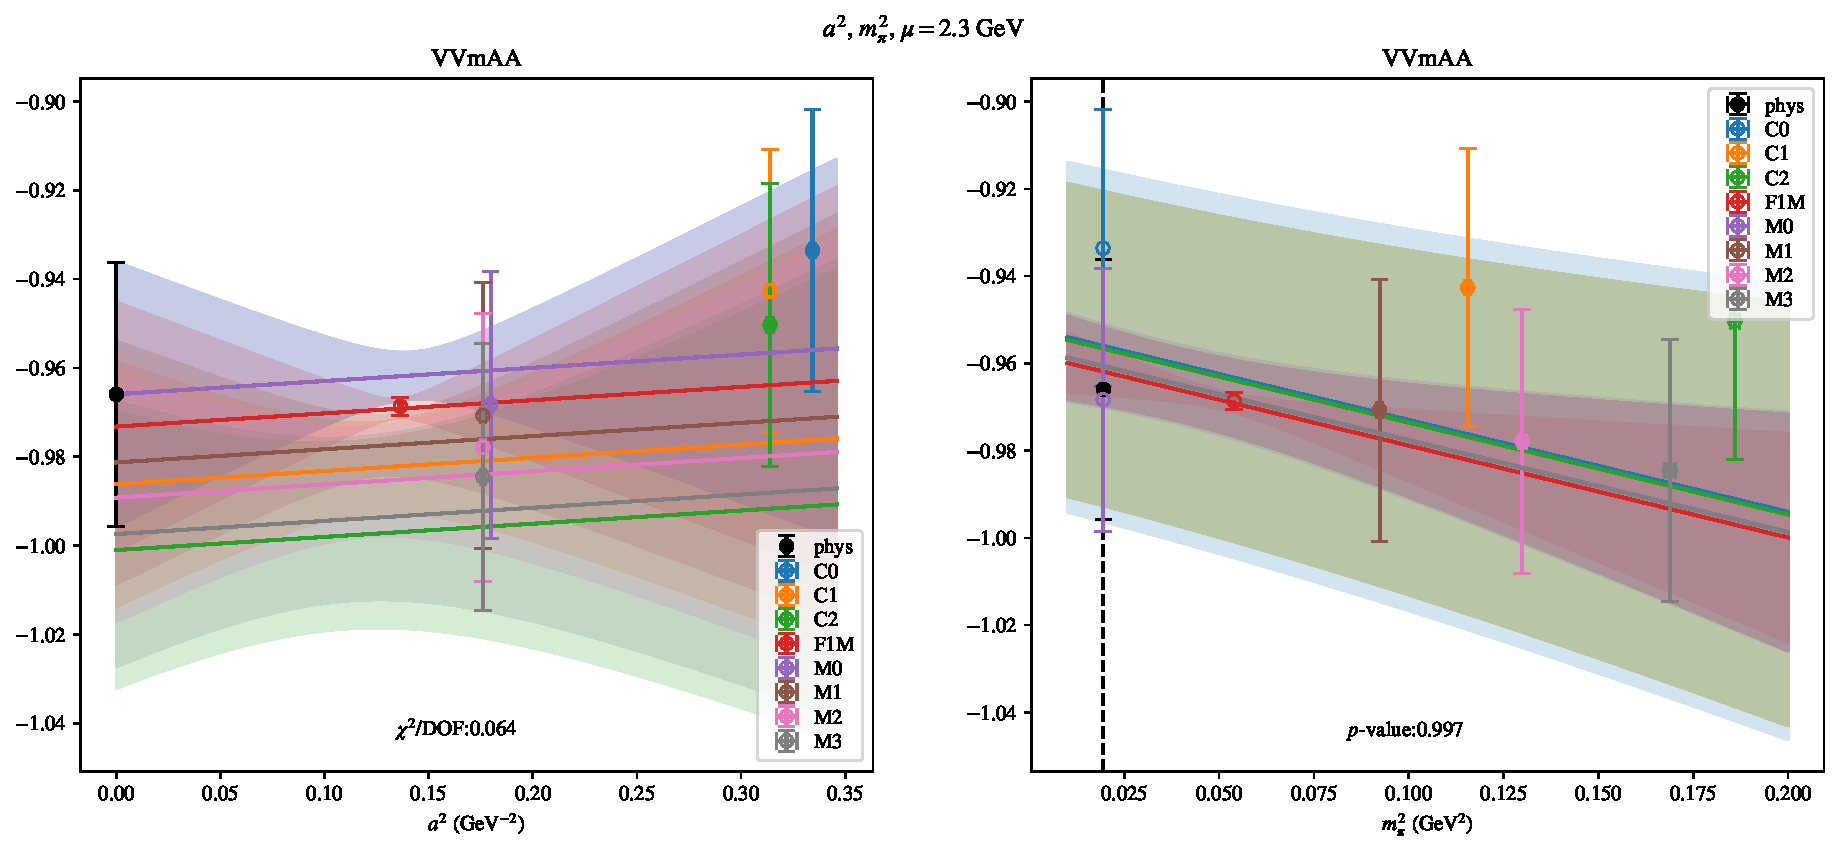
\includepdf[link, pages=-]{VVmAA/NPR/a2m2_23.pdf}
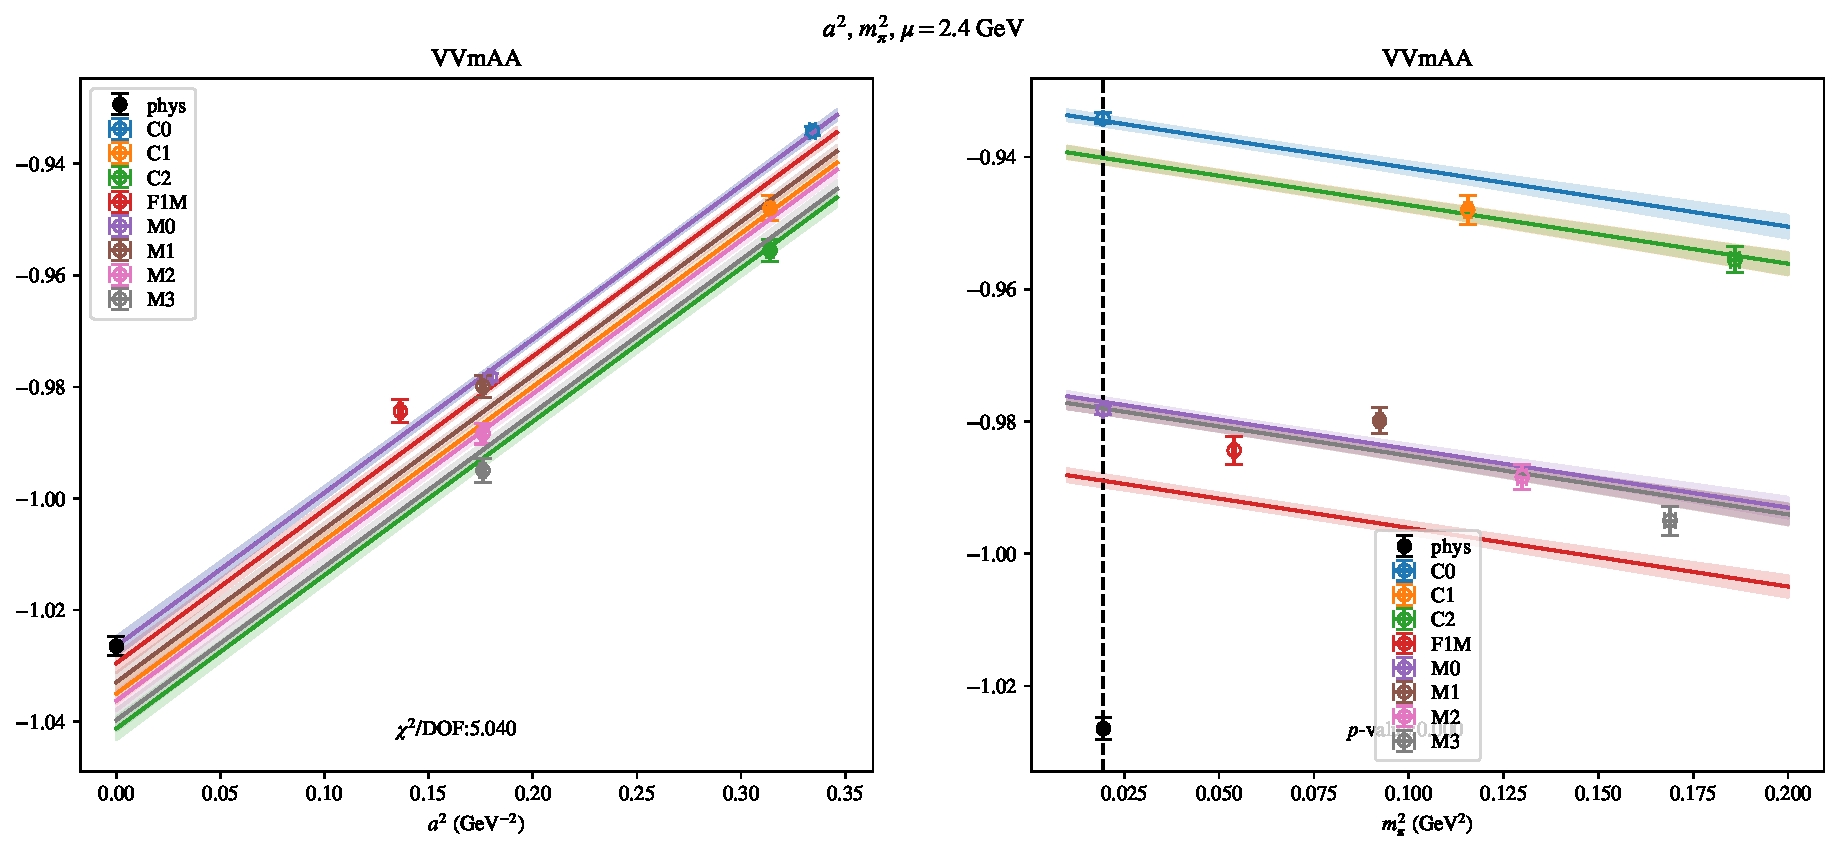
\includepdf[link, pages=-]{VVmAA/NPR/a2m2_24.pdf}
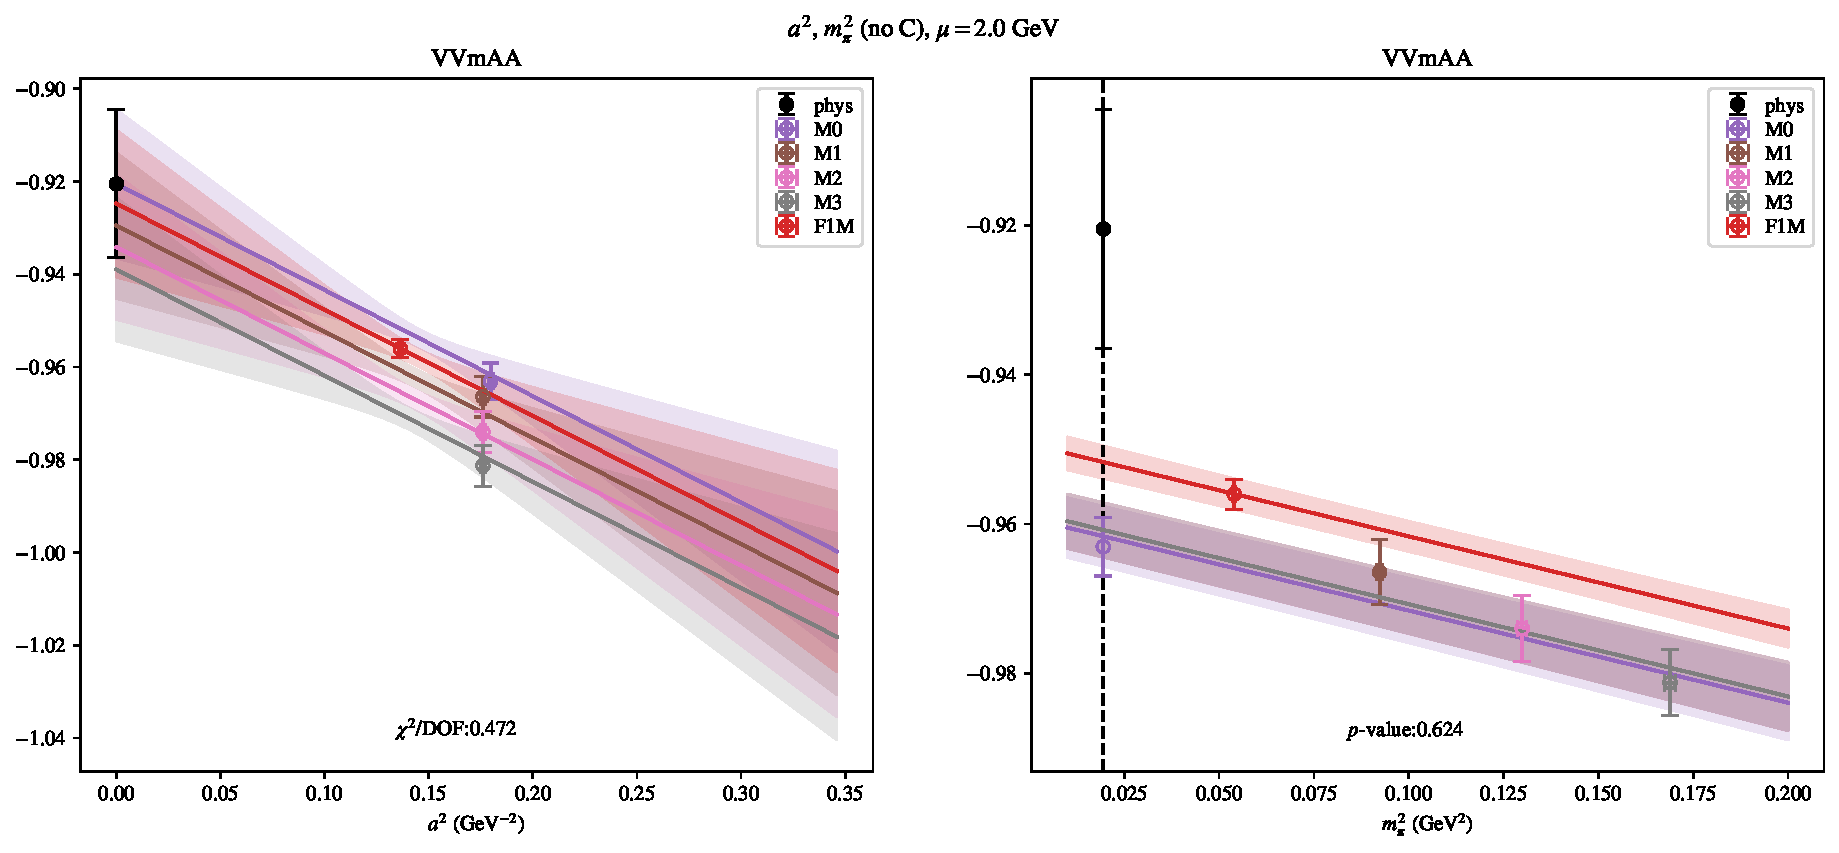
\includepdf[link, pages=-]{VVmAA/NPR/a2m2noC_20.pdf}
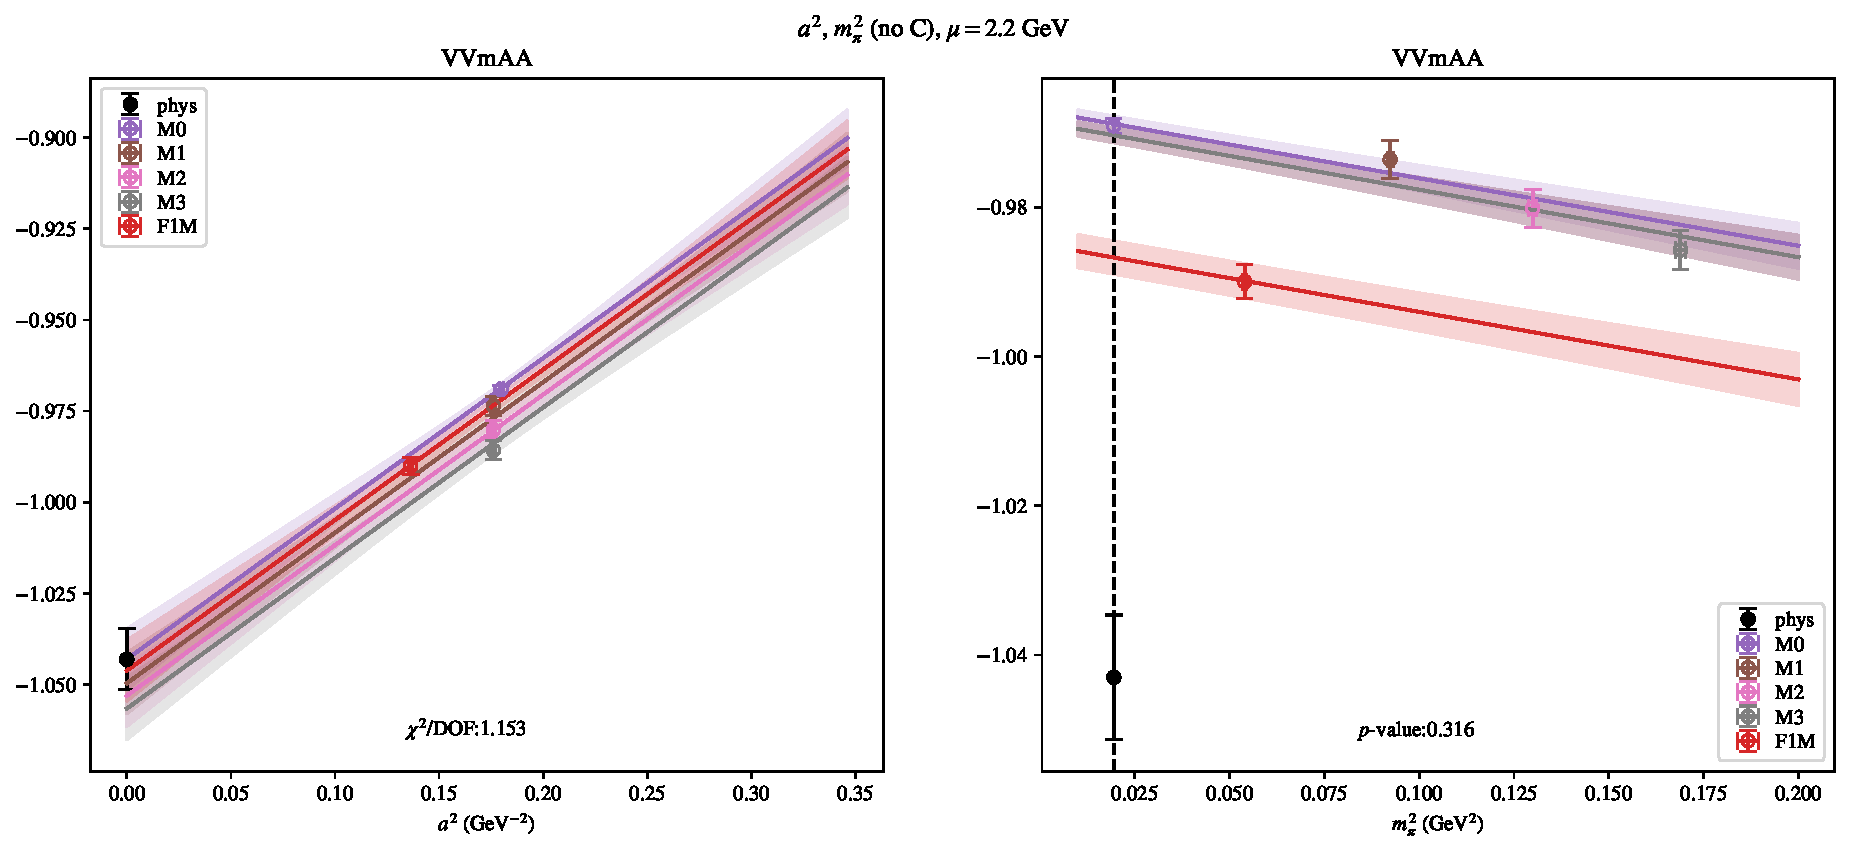
\includepdf[link, pages=-]{VVmAA/NPR/a2m2noC_22.pdf}
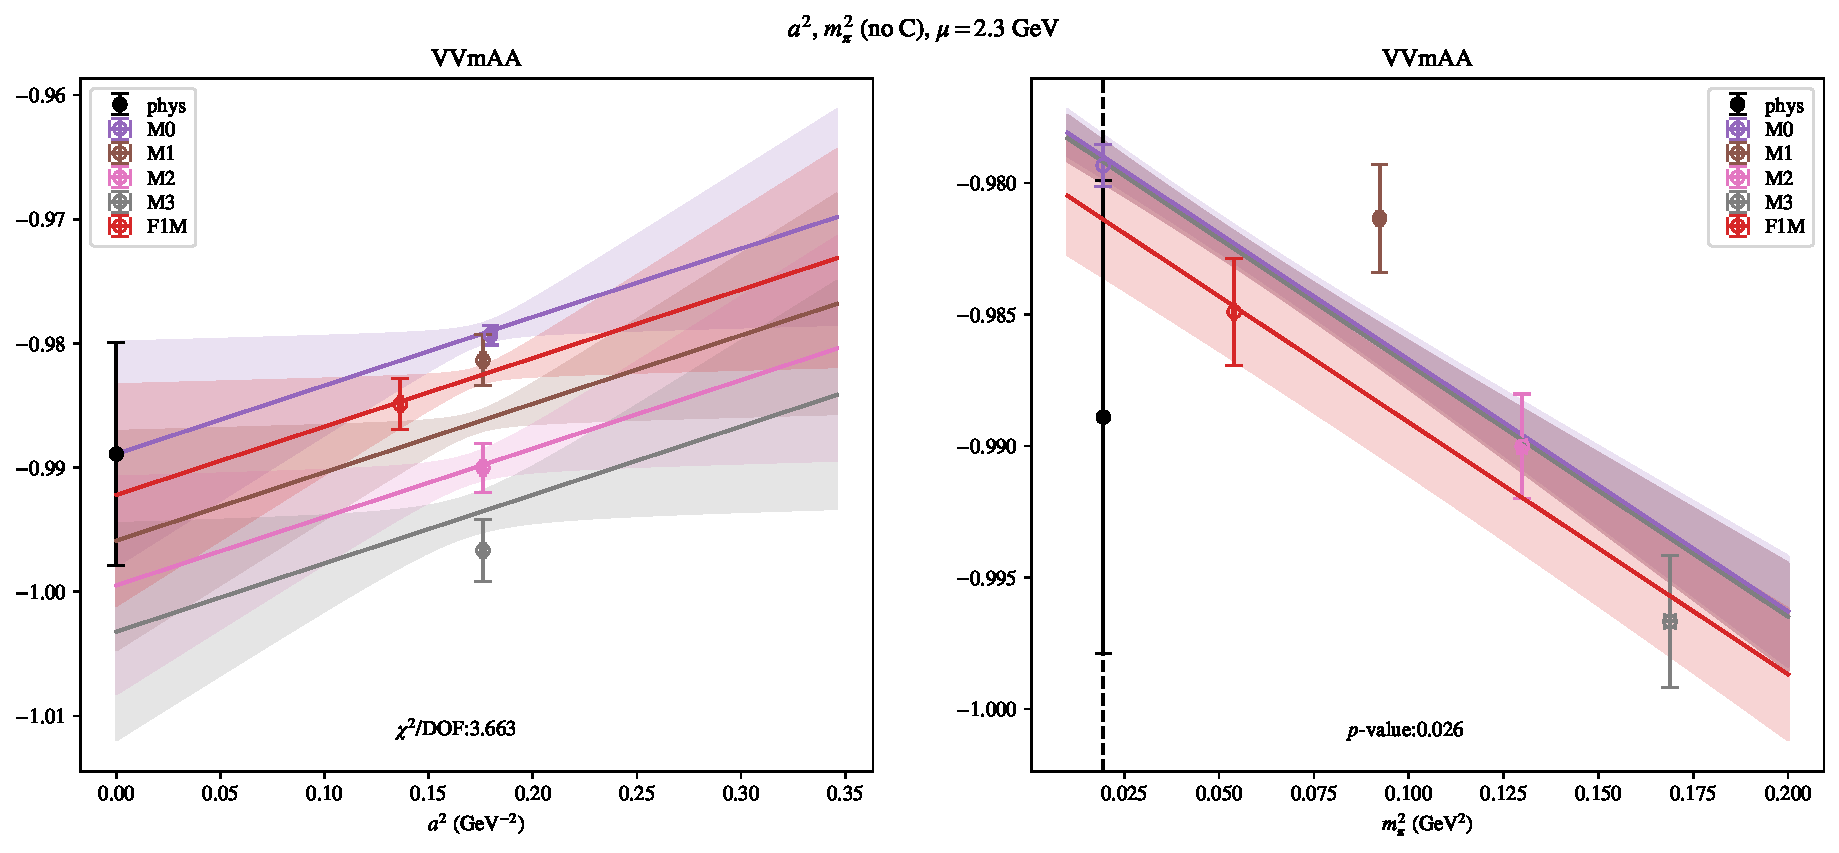
\includepdf[link, pages=-]{VVmAA/NPR/a2m2noC_23.pdf}
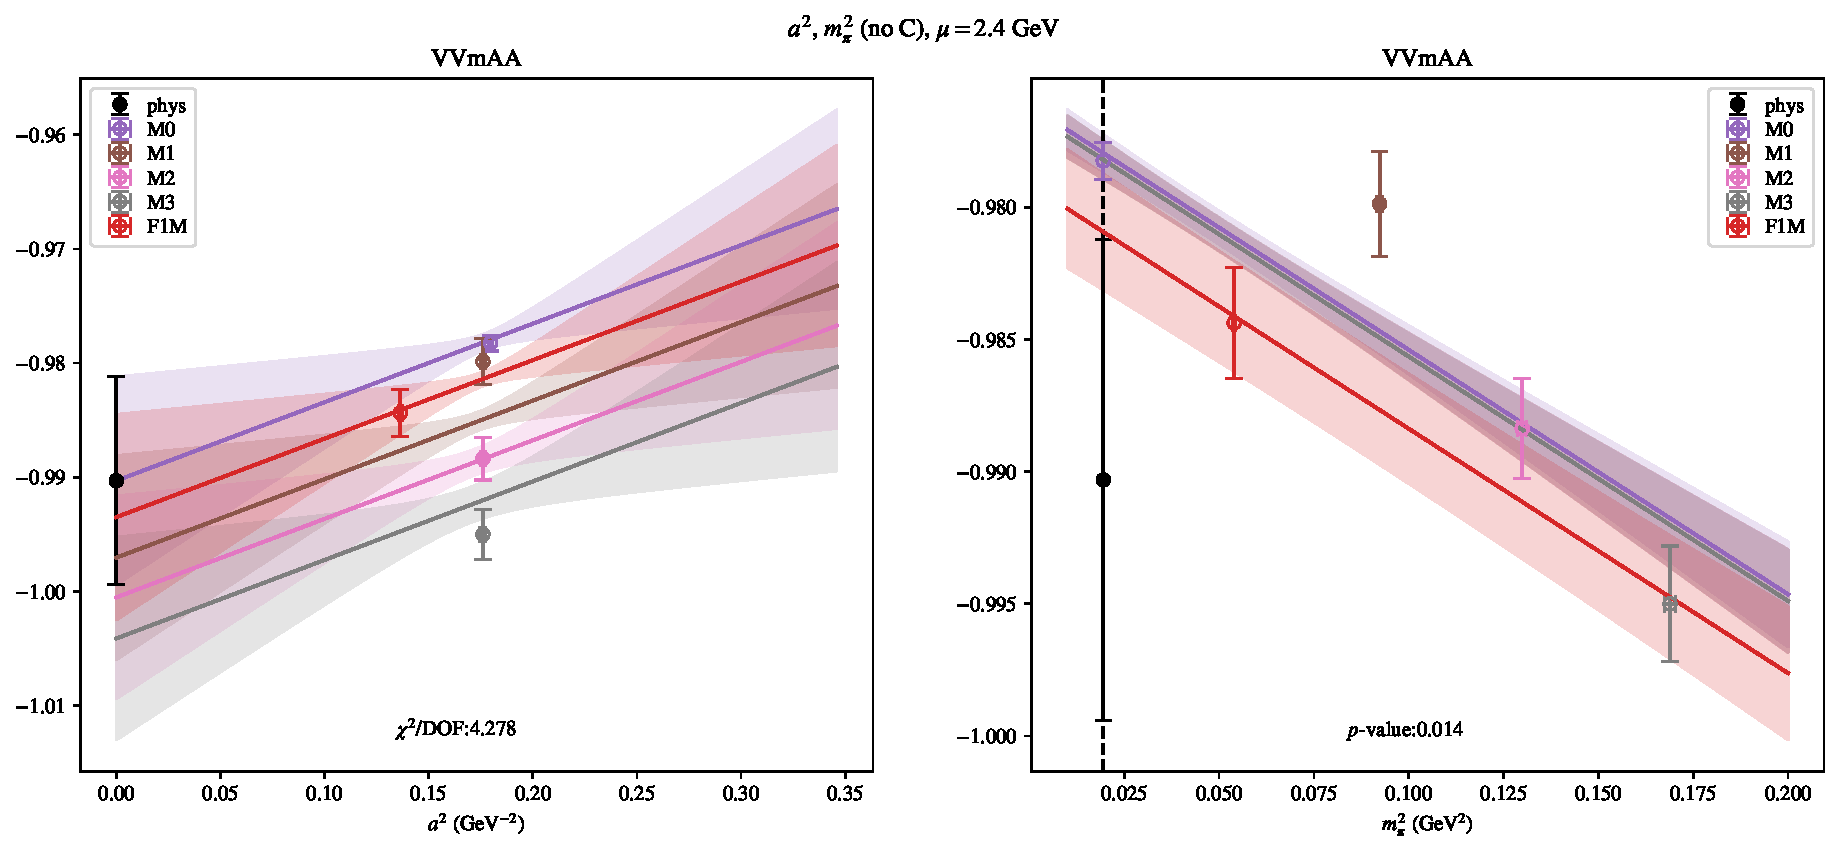
\includepdf[link, pages=-]{VVmAA/NPR/a2m2noC_24.pdf}
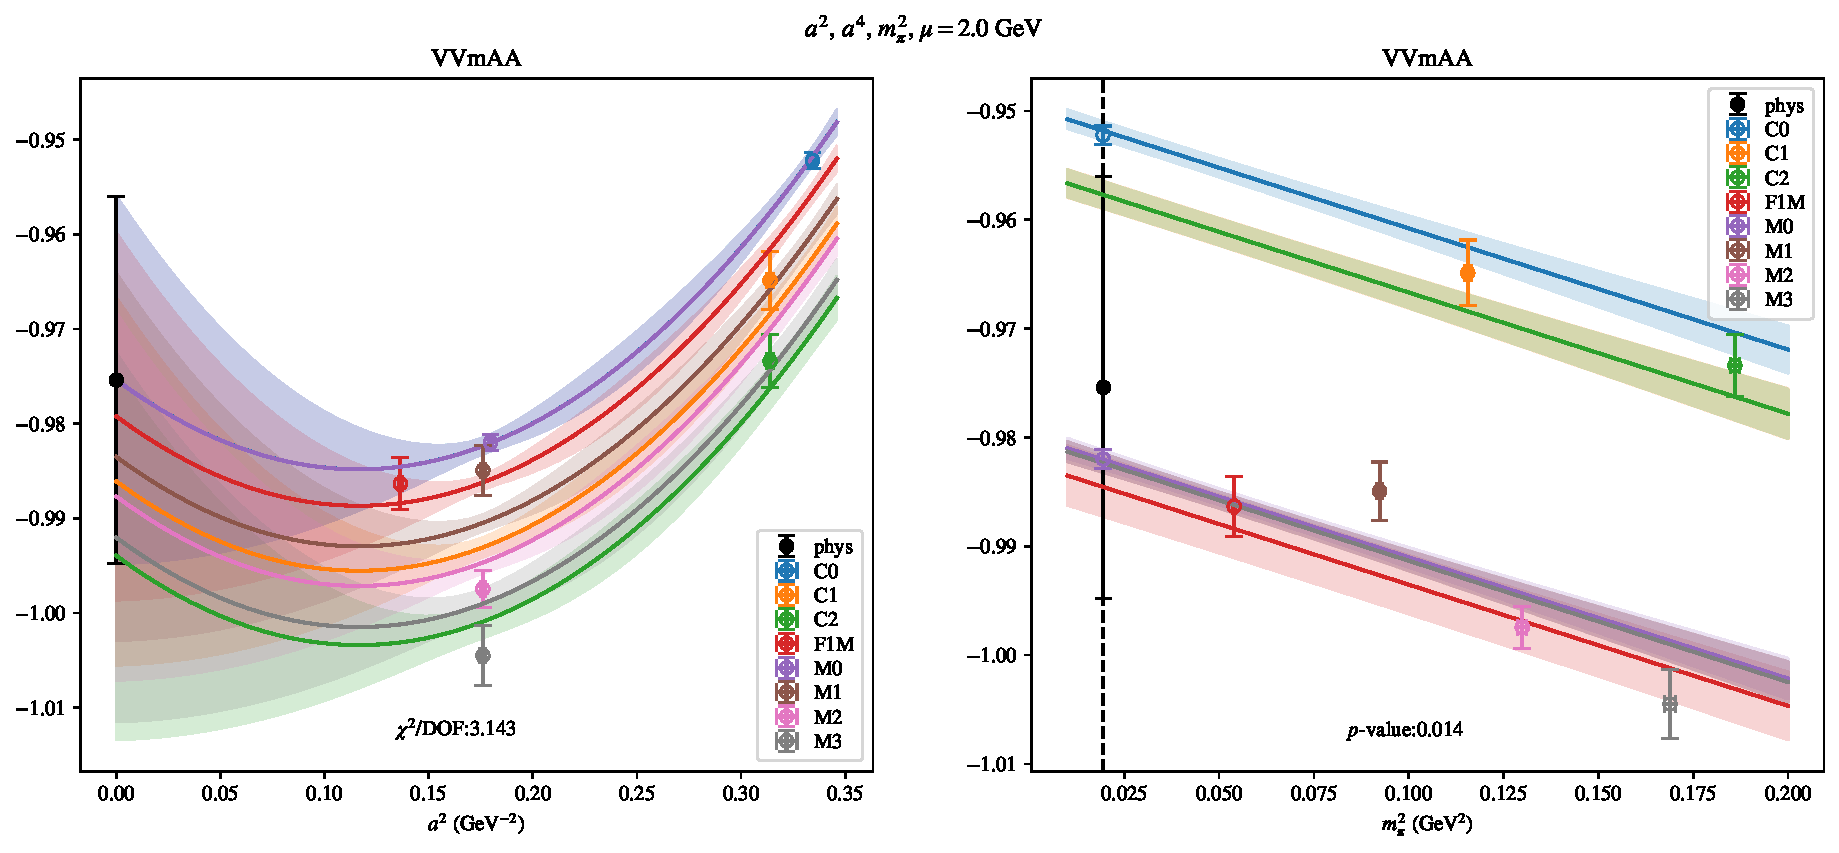
\includepdf[link, pages=-]{VVmAA/NPR/a2a4m2_20.pdf}
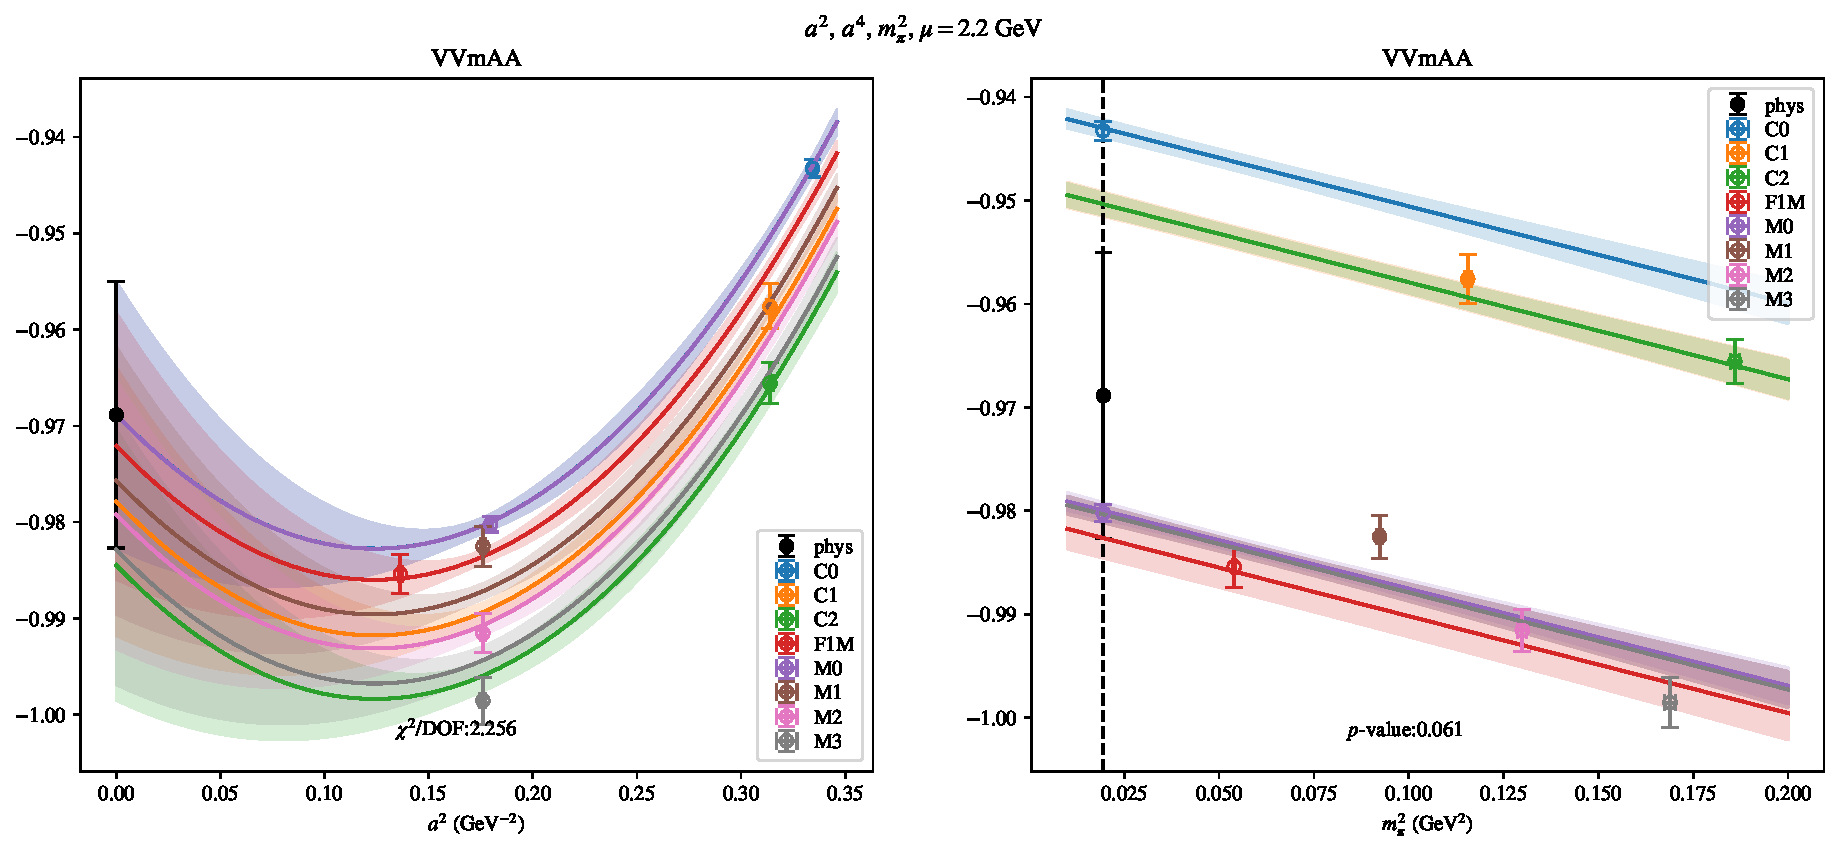
\includepdf[link, pages=-]{VVmAA/NPR/a2a4m2_22.pdf}
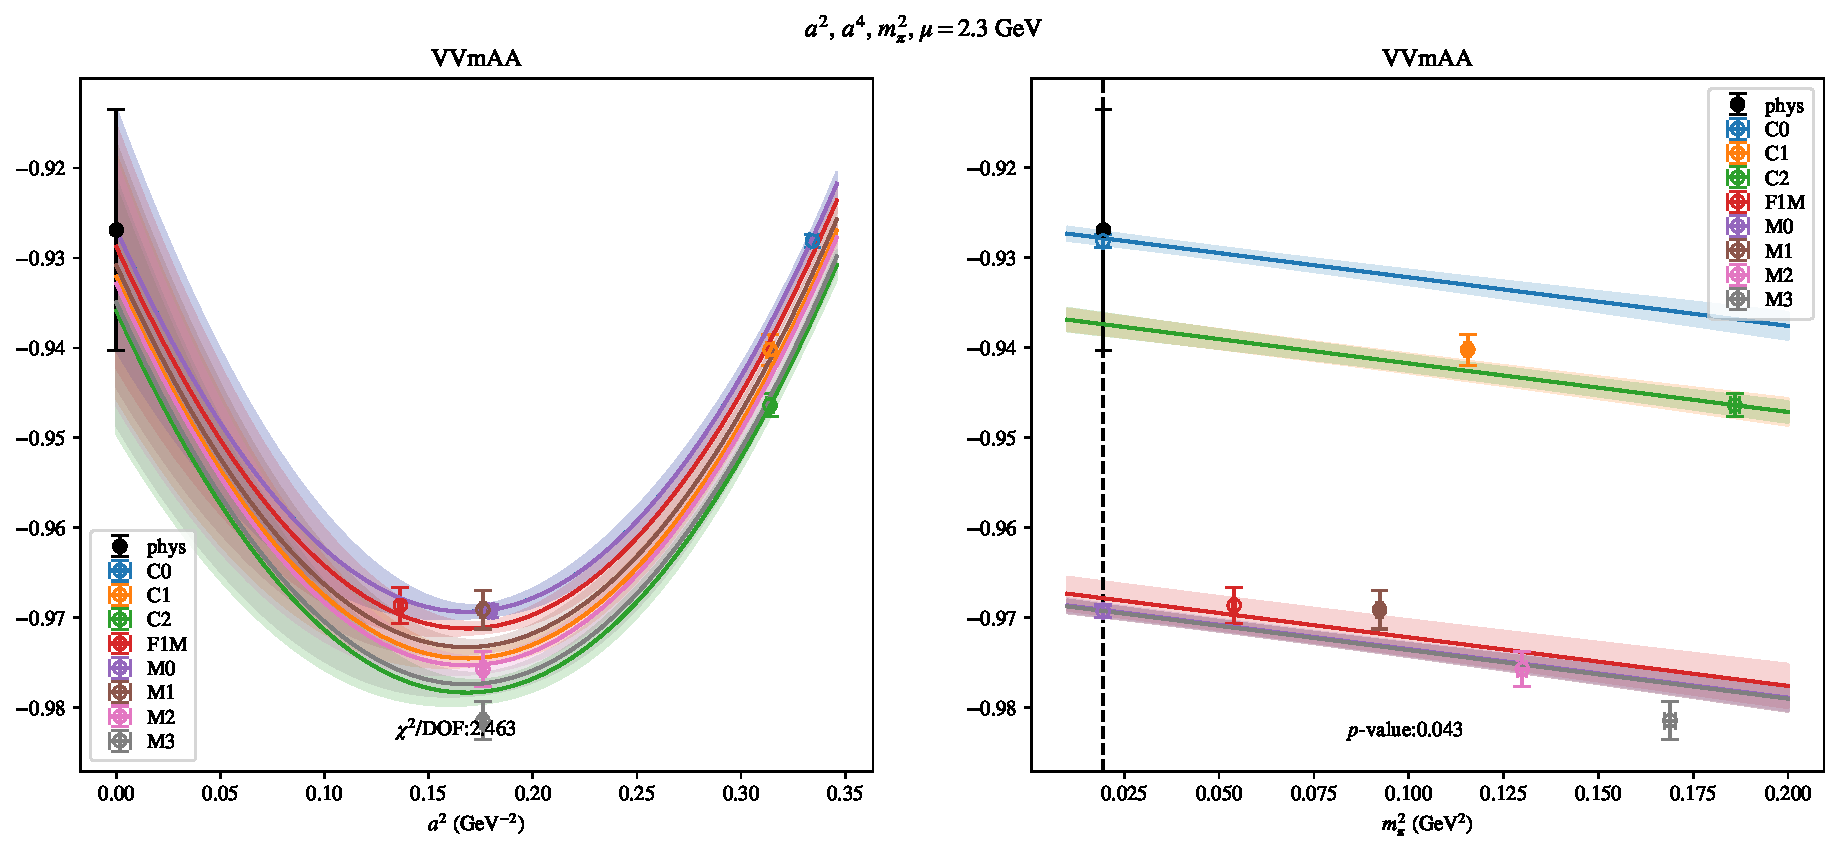
\includepdf[link, pages=-]{VVmAA/NPR/a2a4m2_23.pdf}
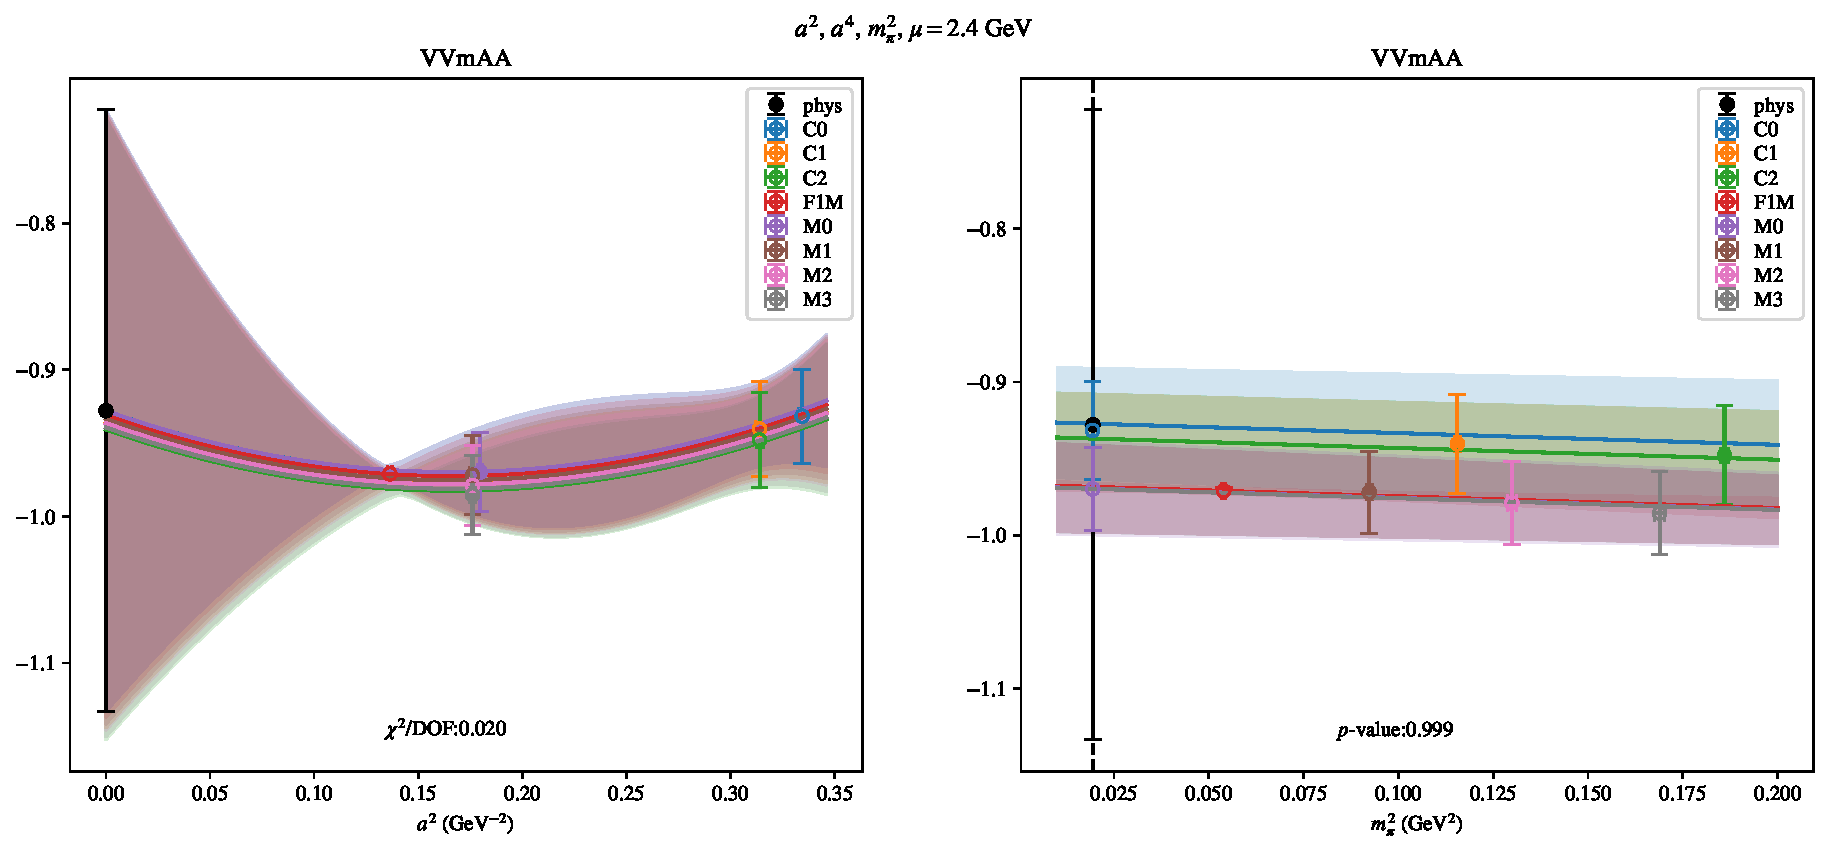
\includepdf[link, pages=-]{VVmAA/NPR/a2a4m2_24.pdf}
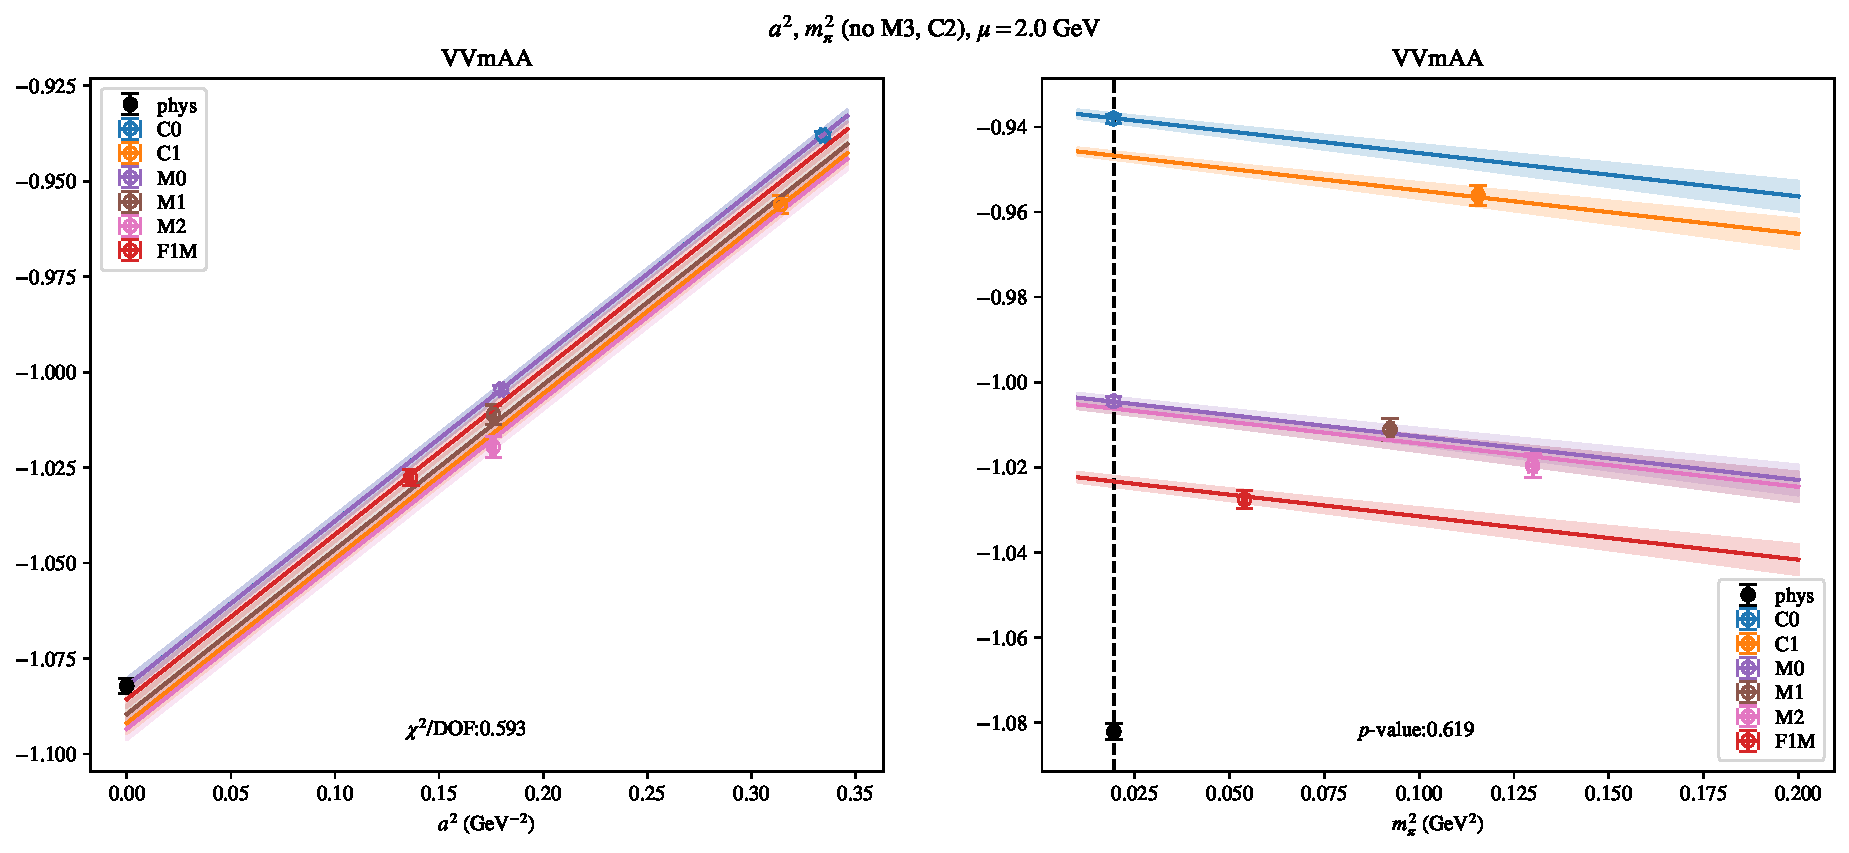
\includepdf[link, pages=-]{VVmAA/NPR/a2m2mcut_20.pdf}
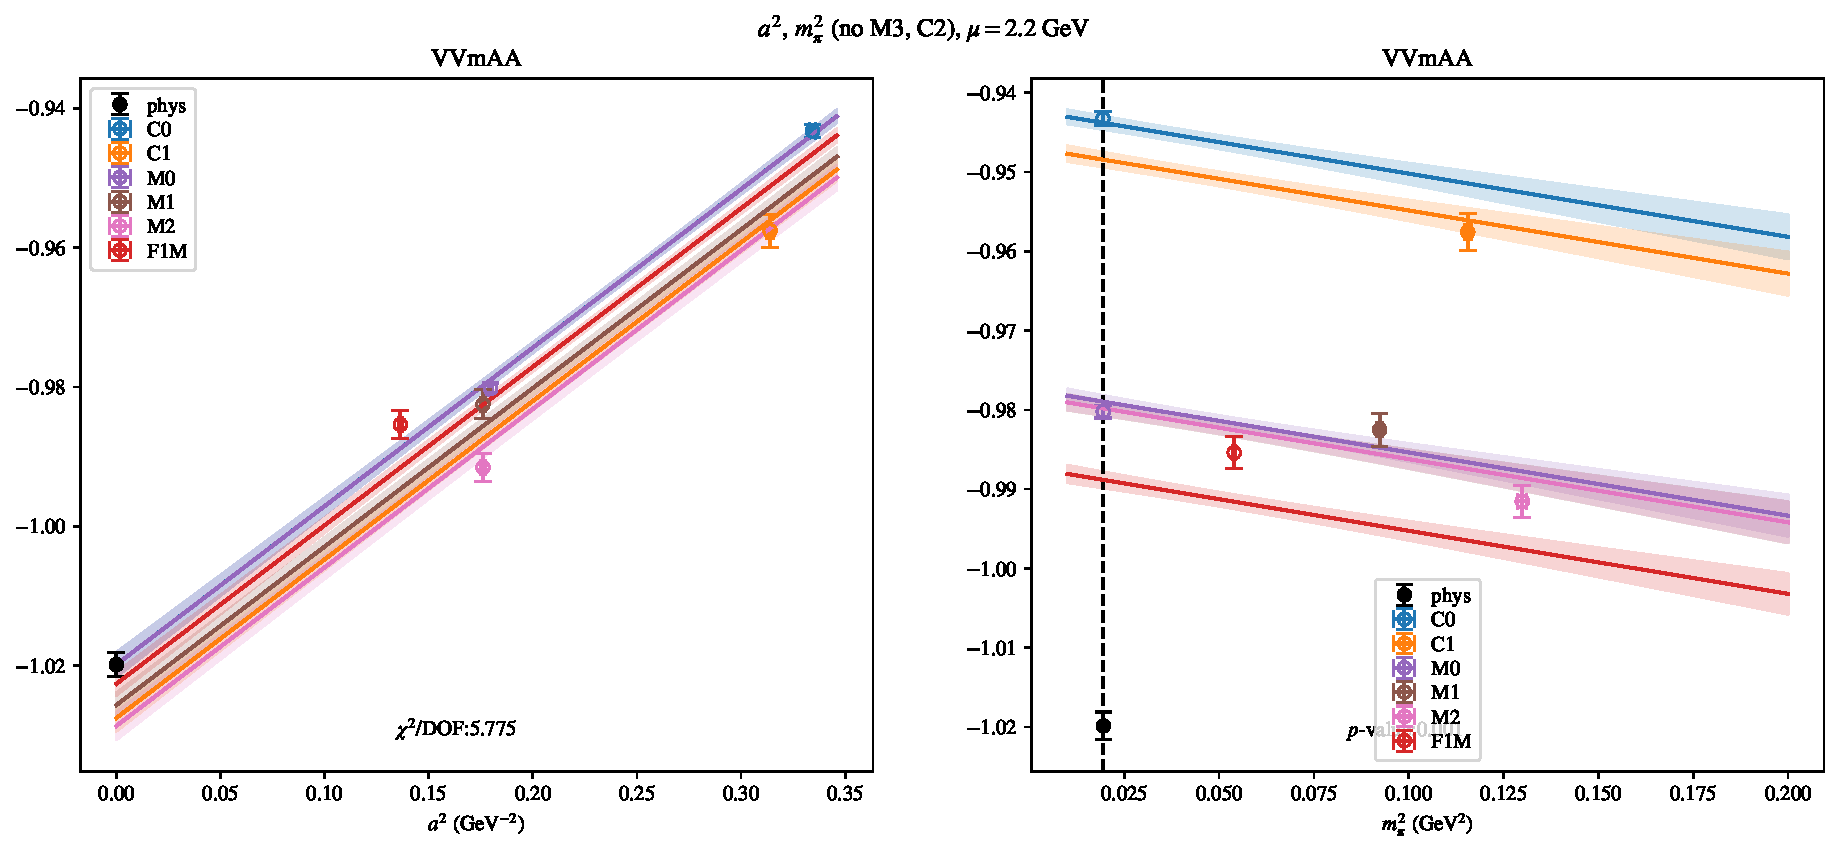
\includepdf[link, pages=-]{VVmAA/NPR/a2m2mcut_22.pdf}
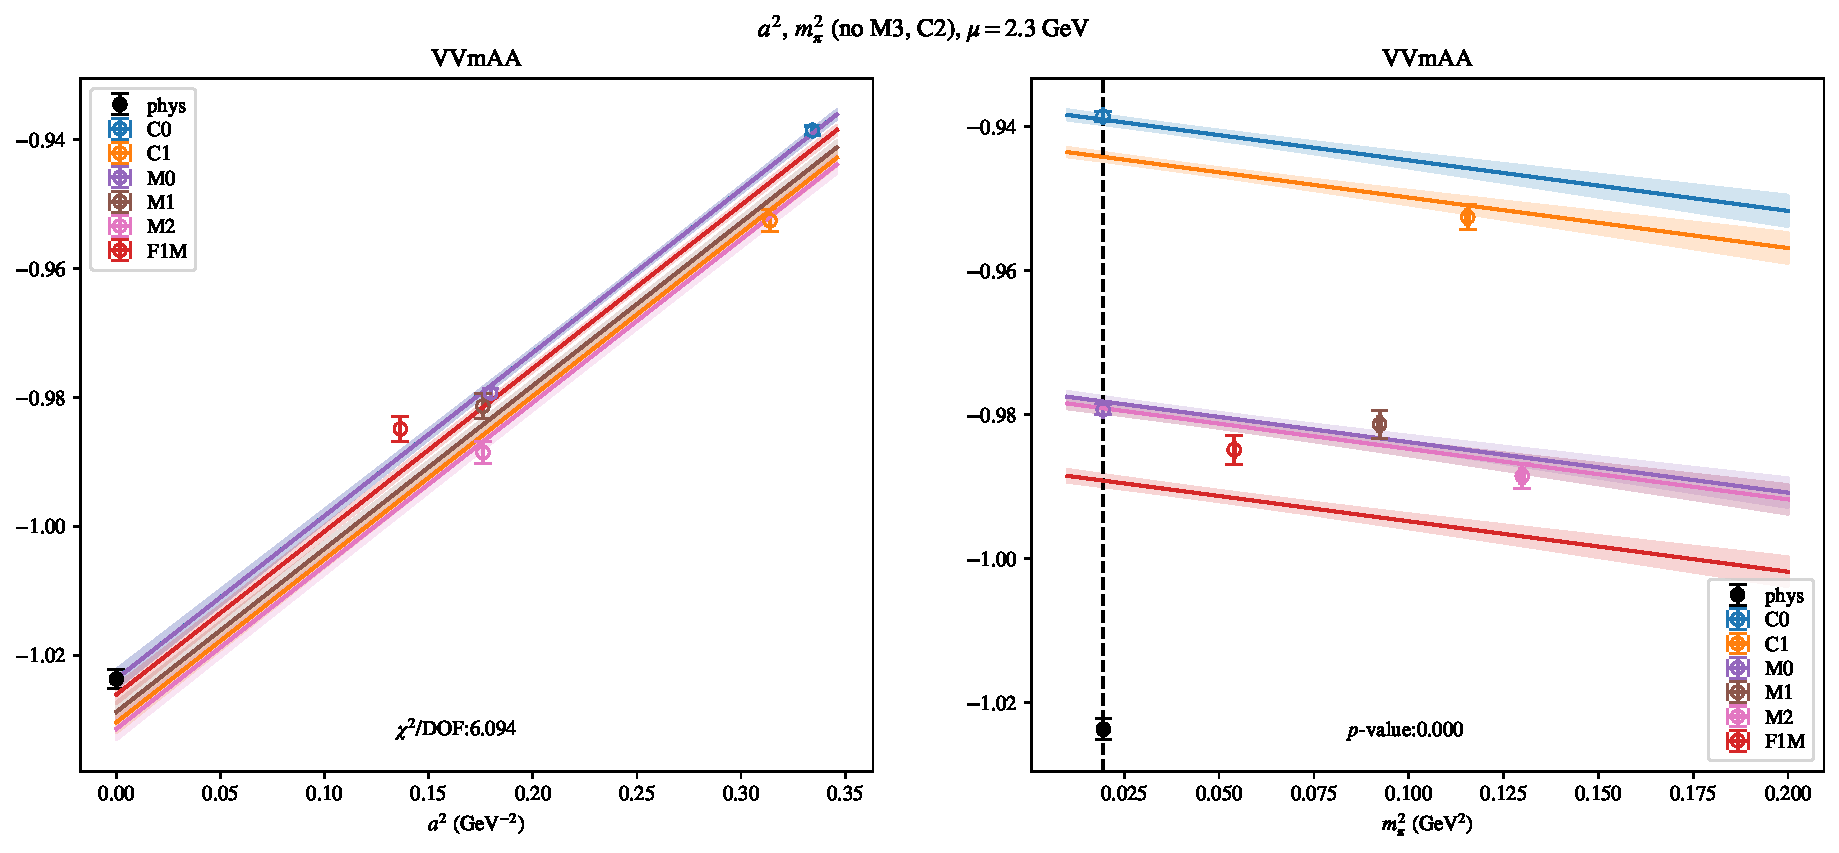
\includepdf[link, pages=-]{VVmAA/NPR/a2m2mcut_23.pdf}
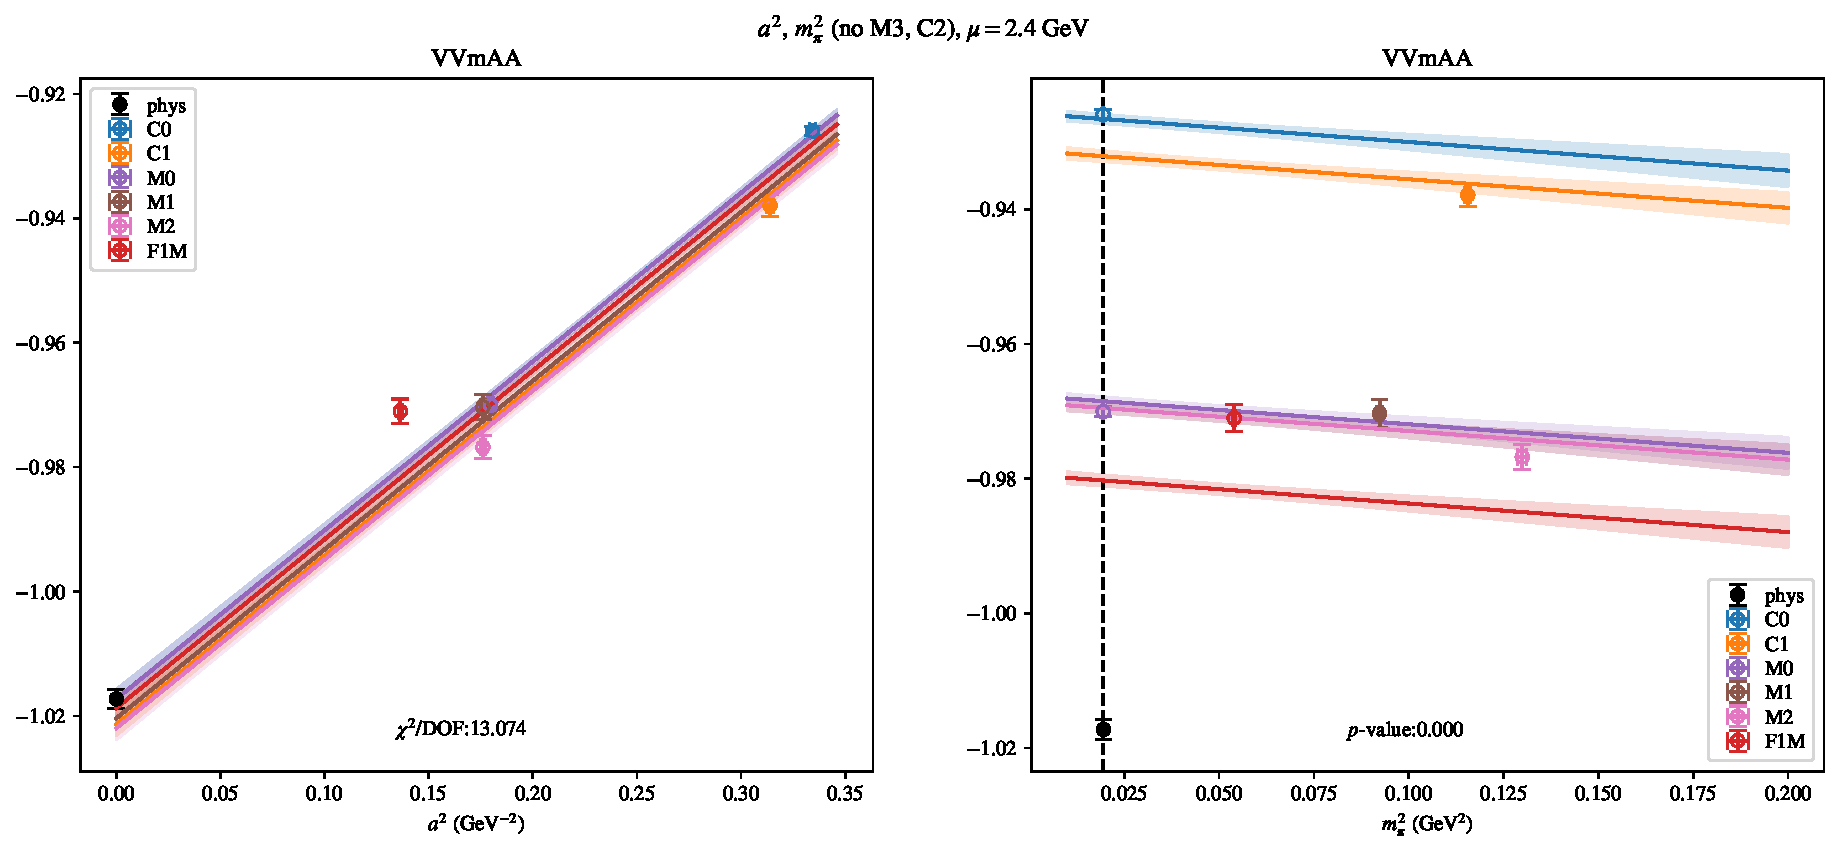
\includepdf[link, pages=-]{VVmAA/NPR/a2m2mcut_24.pdf}
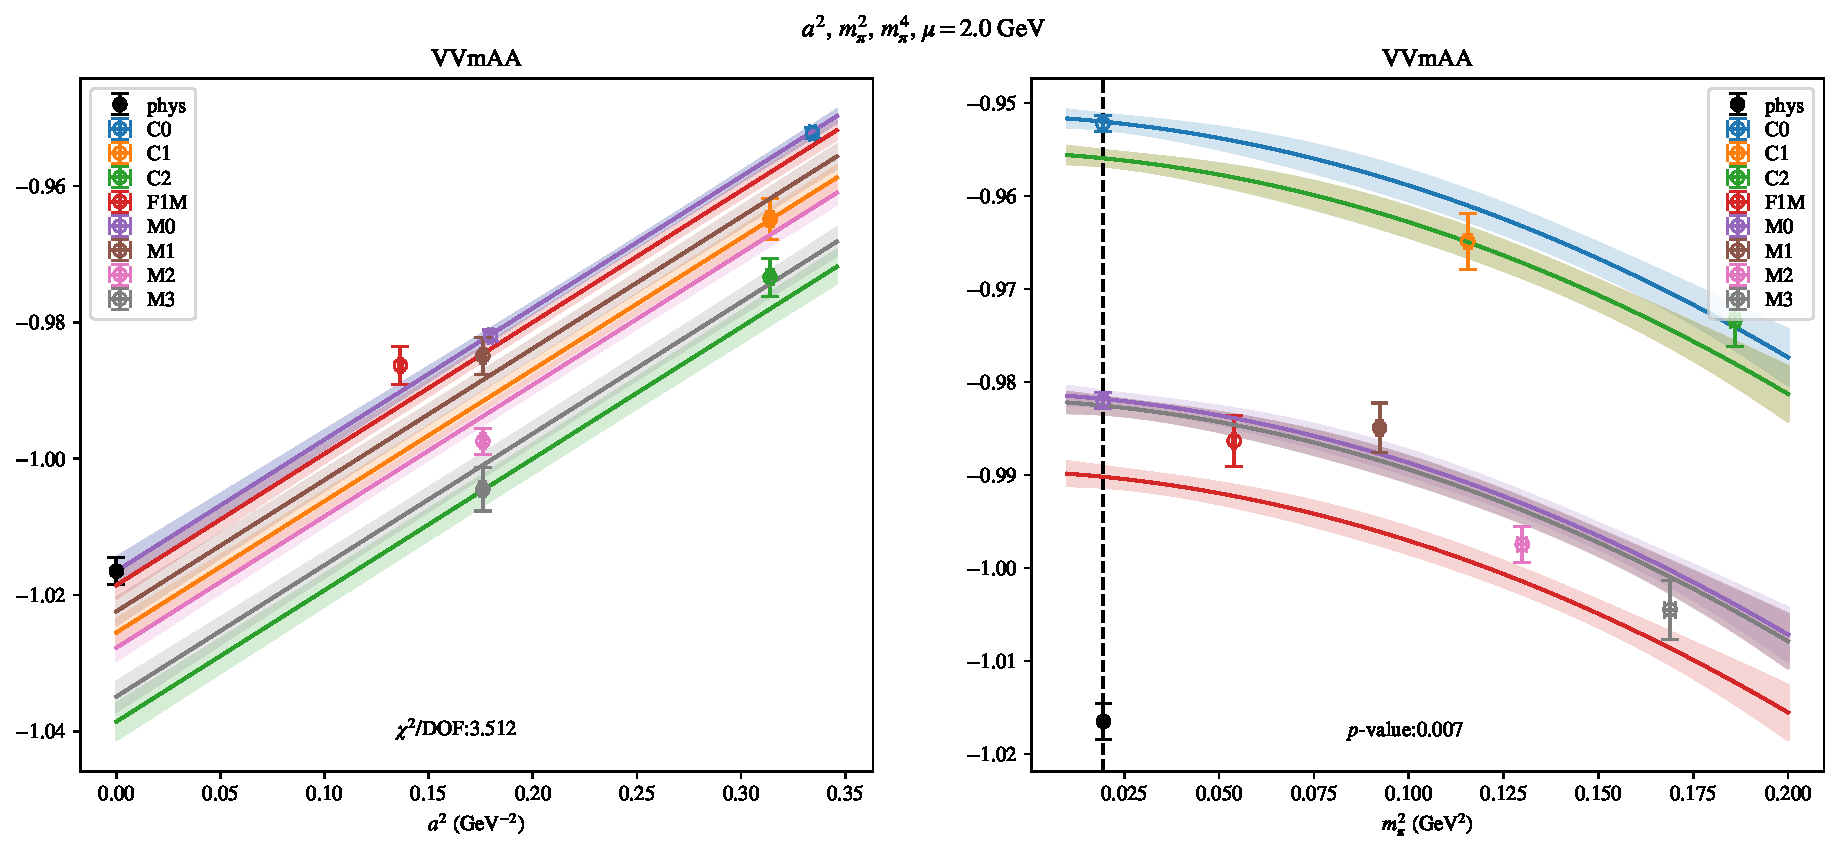
\includepdf[link, pages=-]{VVmAA/NPR/a2m2m4_20.pdf}
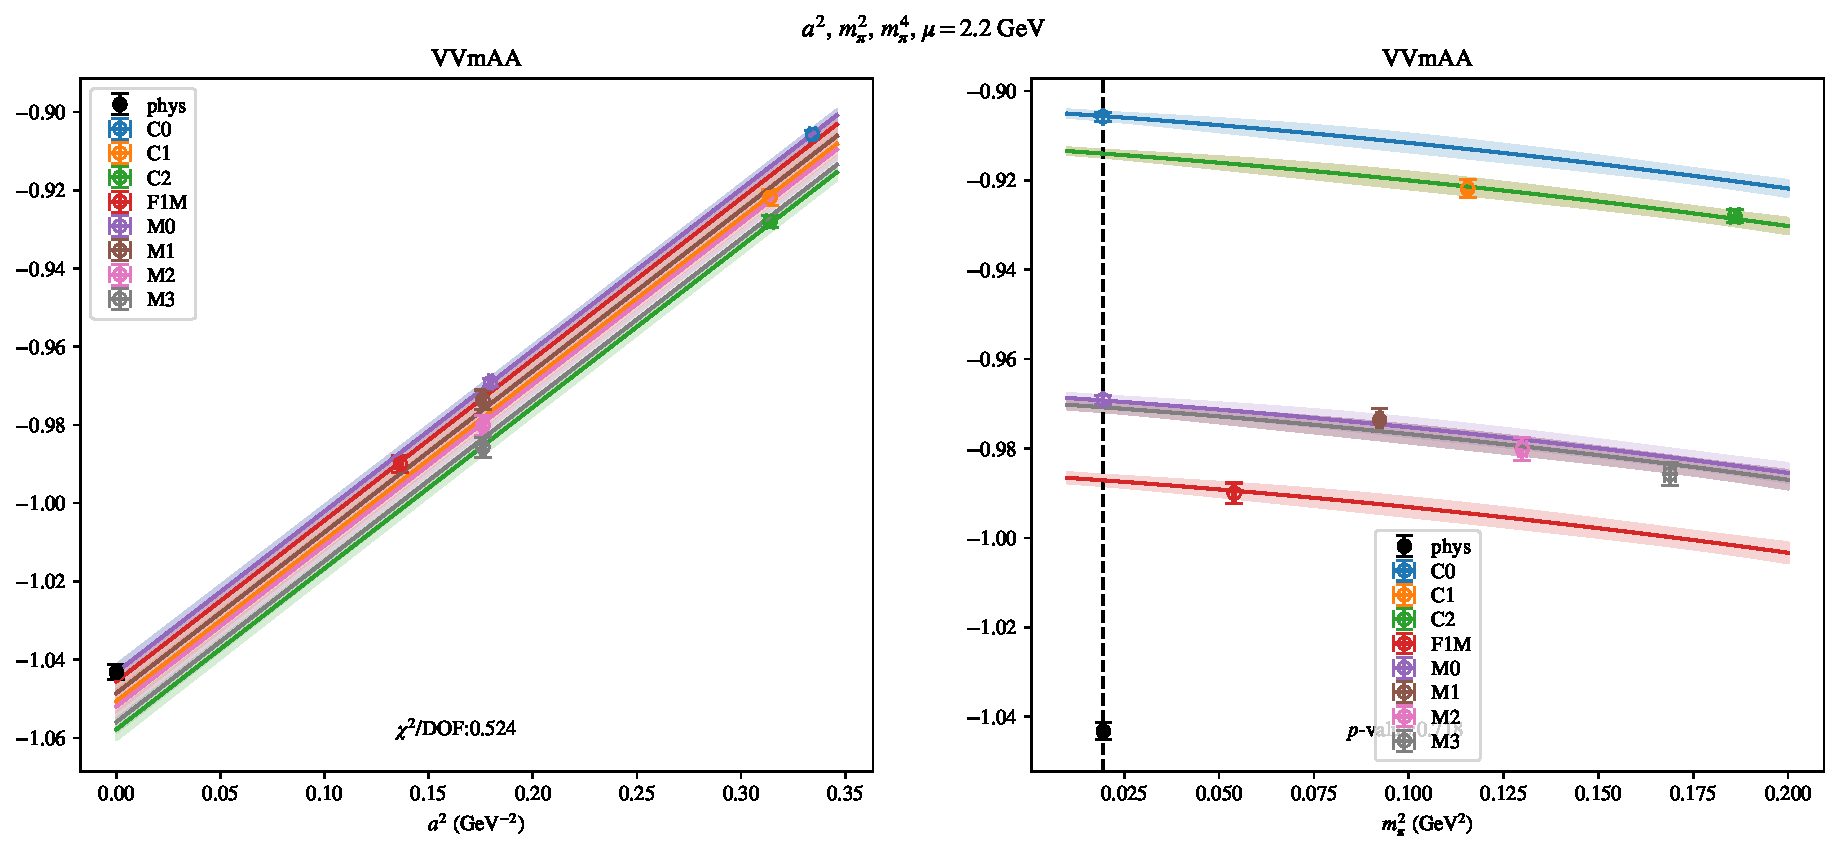
\includepdf[link, pages=-]{VVmAA/NPR/a2m2m4_22.pdf}
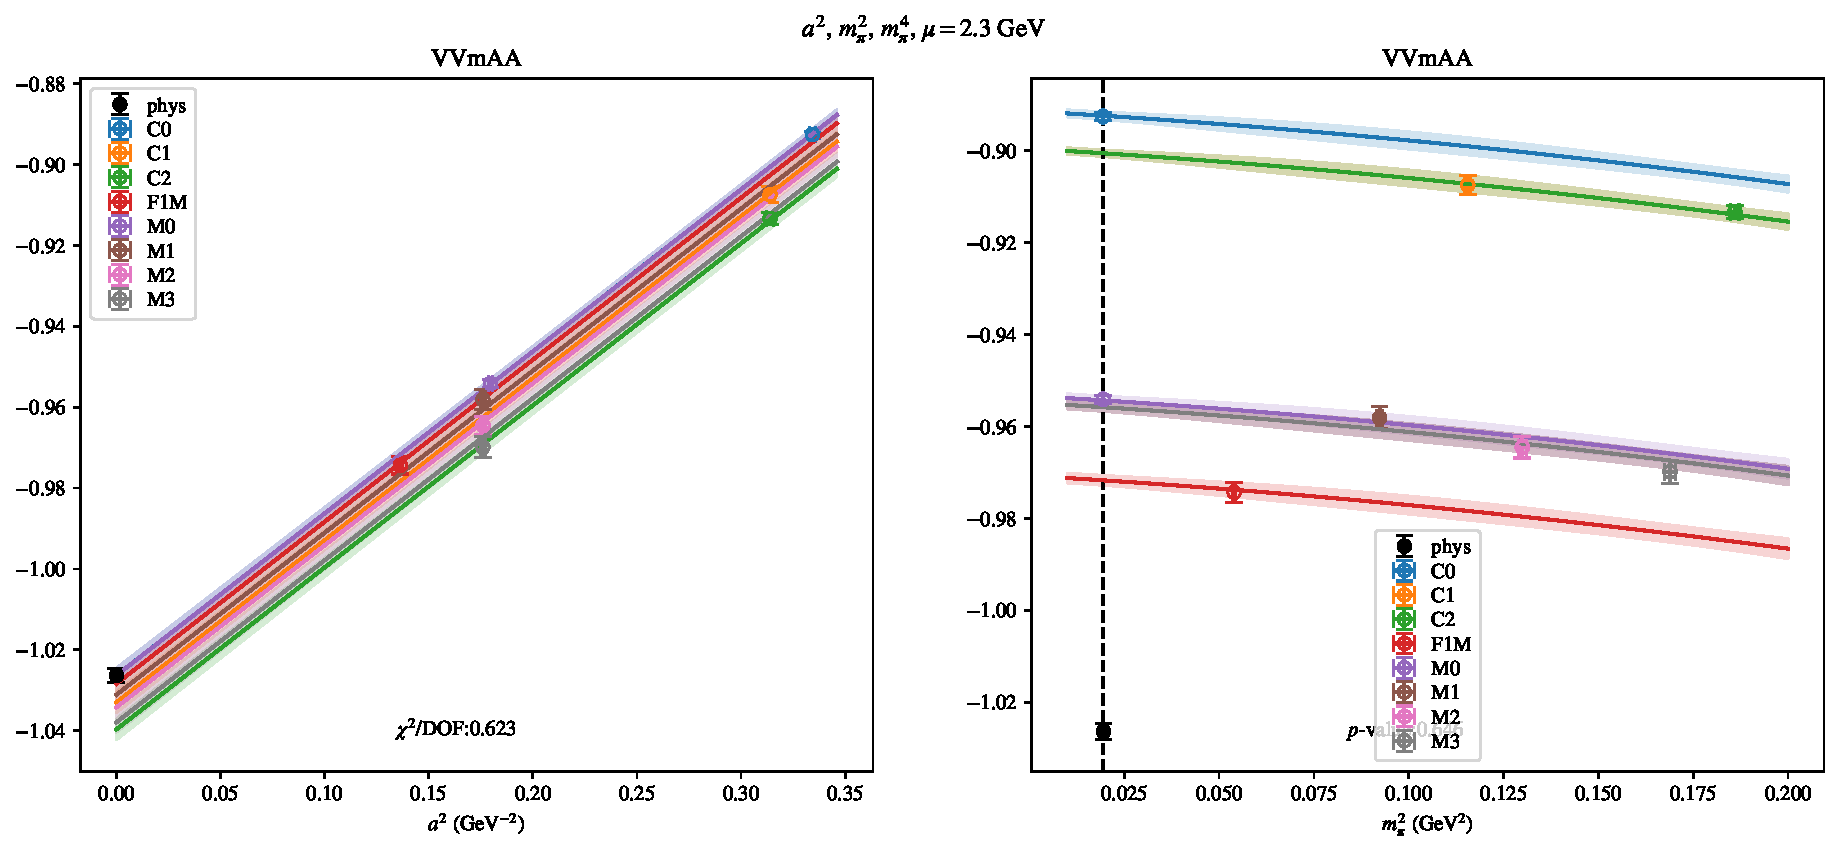
\includepdf[link, pages=-]{VVmAA/NPR/a2m2m4_23.pdf}
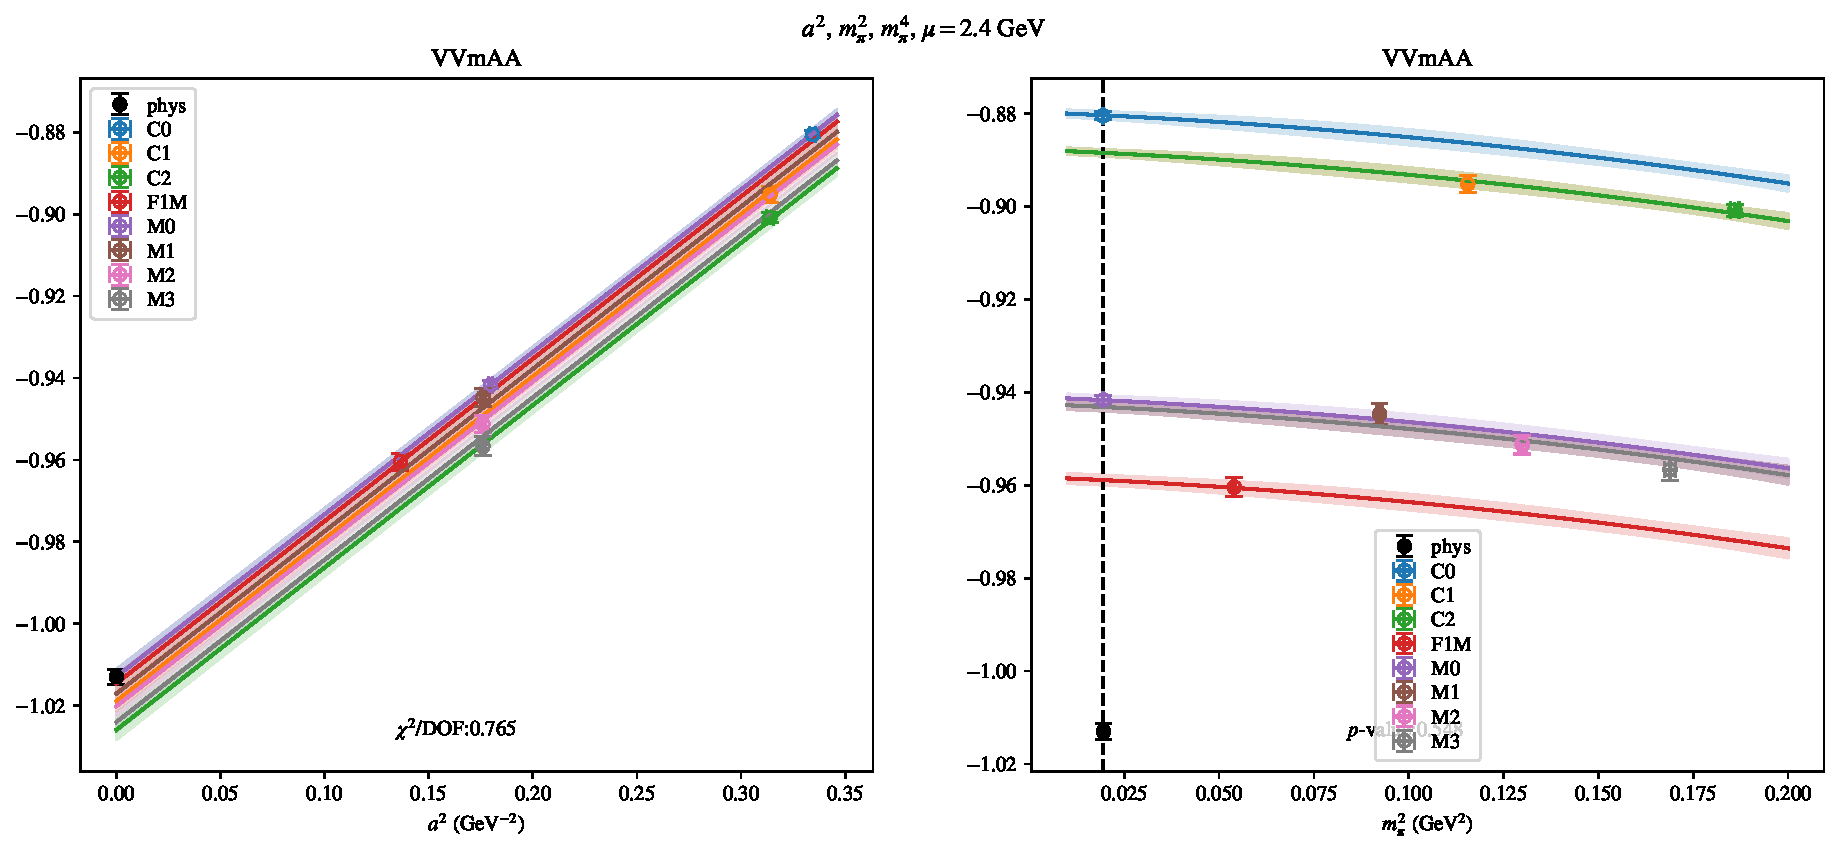
\includepdf[link, pages=-]{VVmAA/NPR/a2m2m4_24.pdf}
\clearpage
\section{$\mathcal{B}_3$}
\begin{table}[h!]
\begin{center}
\begin{tabular}{|c|c|c|c|c|c|}
\hline
$\mu$ (GeV) & $a^2$, $m_\pi^2$& $a^2$, $m_\pi^2$ (no C)& $a^2$, $a^4$, $m_\pi^2$& $a^2$, $m_\pi^2$ (no M3, C2)& $a^2$, $m_\pi^2$, $m_\pi^4$\\
\hline
2.0& \hyperlink{SSmPP/NPR/a2m2_20.pdf.1}{\textbf{1.8412(30)}: 3.492 (0.004)} & \hyperlink{SSmPP/NPR/a2m2noC_20.pdf.1}{\textbf{1.789(13)}: 1.239 (0.29)} & \hyperlink{SSmPP/NPR/a2a4m2_20.pdf.1}{\textbf{1.751(21)}: 0.649 (0.628)} & \hyperlink{SSmPP/NPR/a2m2mcut_20.pdf.1}{\textbf{1.8418(31)}: 5.441 (0.001)} & \hyperlink{SSmPP/NPR/a2m2m4_20.pdf.1}{\textbf{1.8439(31)}: 3.449 (0.008)}\\
2.2& \hyperlink{SSmPP/NPR/a2m2_22.pdf.1}{\textbf{1.8328(27)}: 4.823 (0.0)} & \hyperlink{SSmPP/NPR/a2m2noC_22.pdf.1}{\textbf{1.774(12)}: 1.532 (0.216)} & \hyperlink{SSmPP/NPR/a2a4m2_22.pdf.1}{\textbf{1.735(20)}: 0.941 (0.439)} & \hyperlink{SSmPP/NPR/a2m2mcut_22.pdf.1}{\textbf{1.8334(29)}: 7.378 (0.0)} & \hyperlink{SSmPP/NPR/a2m2m4_22.pdf.1}{\textbf{1.8360(30)}: 4.679 (0.001)}\\
2.3& \hyperlink{SSmPP/NPR/a2m2_23.pdf.1}{\textbf{1.8298(27)}: 5.259 (0.0)} & \hyperlink{SSmPP/NPR/a2m2noC_23.pdf.1}{\textbf{1.769(12)}: 1.673 (0.188)} & \hyperlink{SSmPP/NPR/a2a4m2_23.pdf.1}{\textbf{1.730(20)}: 1.118 (0.346)} & \hyperlink{SSmPP/NPR/a2m2mcut_23.pdf.1}{\textbf{1.8304(29)}: 7.94 (0.0)} & \hyperlink{SSmPP/NPR/a2m2m4_23.pdf.1}{\textbf{1.8332(29)}: 5.007 (0.0)}\\
2.4& \hyperlink{SSmPP/NPR/a2m2_24.pdf.1}{\textbf{1.8275(27)}: 5.913 (0.0)} & \hyperlink{SSmPP/NPR/a2m2noC_24.pdf.1}{\textbf{1.764(12)}: 1.872 (0.154)} & \hyperlink{SSmPP/NPR/a2a4m2_24.pdf.1}{\textbf{1.722(20)}: 1.195 (0.311)} & \hyperlink{SSmPP/NPR/a2m2mcut_24.pdf.1}{\textbf{1.8283(29)}: 8.899 (0.0)} & \hyperlink{SSmPP/NPR/a2m2m4_24.pdf.1}{\textbf{1.8312(29)}: 5.498 (0.0)}\\
\hline
\end{tabular}
\caption{Physical point value from chiral and continuum extrapolation at renormalisation scale $\mu$. Entries are \textbf{value(error)}: $\chi^2/\text{DOF}$ ($p$-value).}
\end{center}
\end{table}
\begin{table}[h!]
\begin{center}
\begin{tabular}{|c c|c|c|c|c|c|}
\hline
$\mu$ (GeV) &  & $a^2$, $m_\pi^2$& $a^2$, $m_\pi^2$ (no C)& $a^2$, $a^4$, $m_\pi^2$& $a^2$, $m_\pi^2$ (no M3, C2)& $a^2$, $m_\pi^2$, $m_\pi^4$\\
\hline
\multirow{2}{0.5in}{2.0} & $\alpha$ & 0.0715(55)& 0.242(42)& 0.53(11)& 0.0706(59)& 0.0668(59)\\
 & $\beta$ & -0.0001(11)& -0.0002(21)& -0.0003(13)& -0.0003(21)& -0.0014(63)\\
\hline
\multirow{2}{0.5in}{2.2} & $\alpha$ & 0.0725(54)& 0.268(42)& 0.58(11)& 0.0718(58)& 0.0667(58)\\
 & $\beta$ & -0.0002(11)& -0.0003(20)& -0.0004(12)& -0.0004(20)& -0.0017(61)\\
\hline
\multirow{2}{0.5in}{2.3} & $\alpha$ & 0.0736(53)& 0.276(42)& 0.59(11)& 0.0729(58)& 0.0675(58)\\
 & $\beta$ & -0.0003(11)& -0.0003(20)& -0.0005(12)& -0.0005(20)& -0.0019(61)\\
\hline
\multirow{2}{0.5in}{2.4} & $\alpha$ & 0.0745(53)& 0.287(43)& 0.62(11)& 0.0733(58)& 0.0678(58)\\
 & $\beta$ & -0.0003(11)& -0.0004(19)& -0.0005(12)& -0.0006(20)& -0.0020(61)\\
\hline
\end{tabular}
\caption{Fit values of coefficients in $Q = Q_{phys} + \mathbf{\alpha} a^2 + \mathbf{\beta}\left(\frac{m_\pi^2}{f_\pi^2}-\frac{m_{\pi,PDG}^2}{f_\pi^2}\right) + \ldots$.}
\end{center}
\end{table}
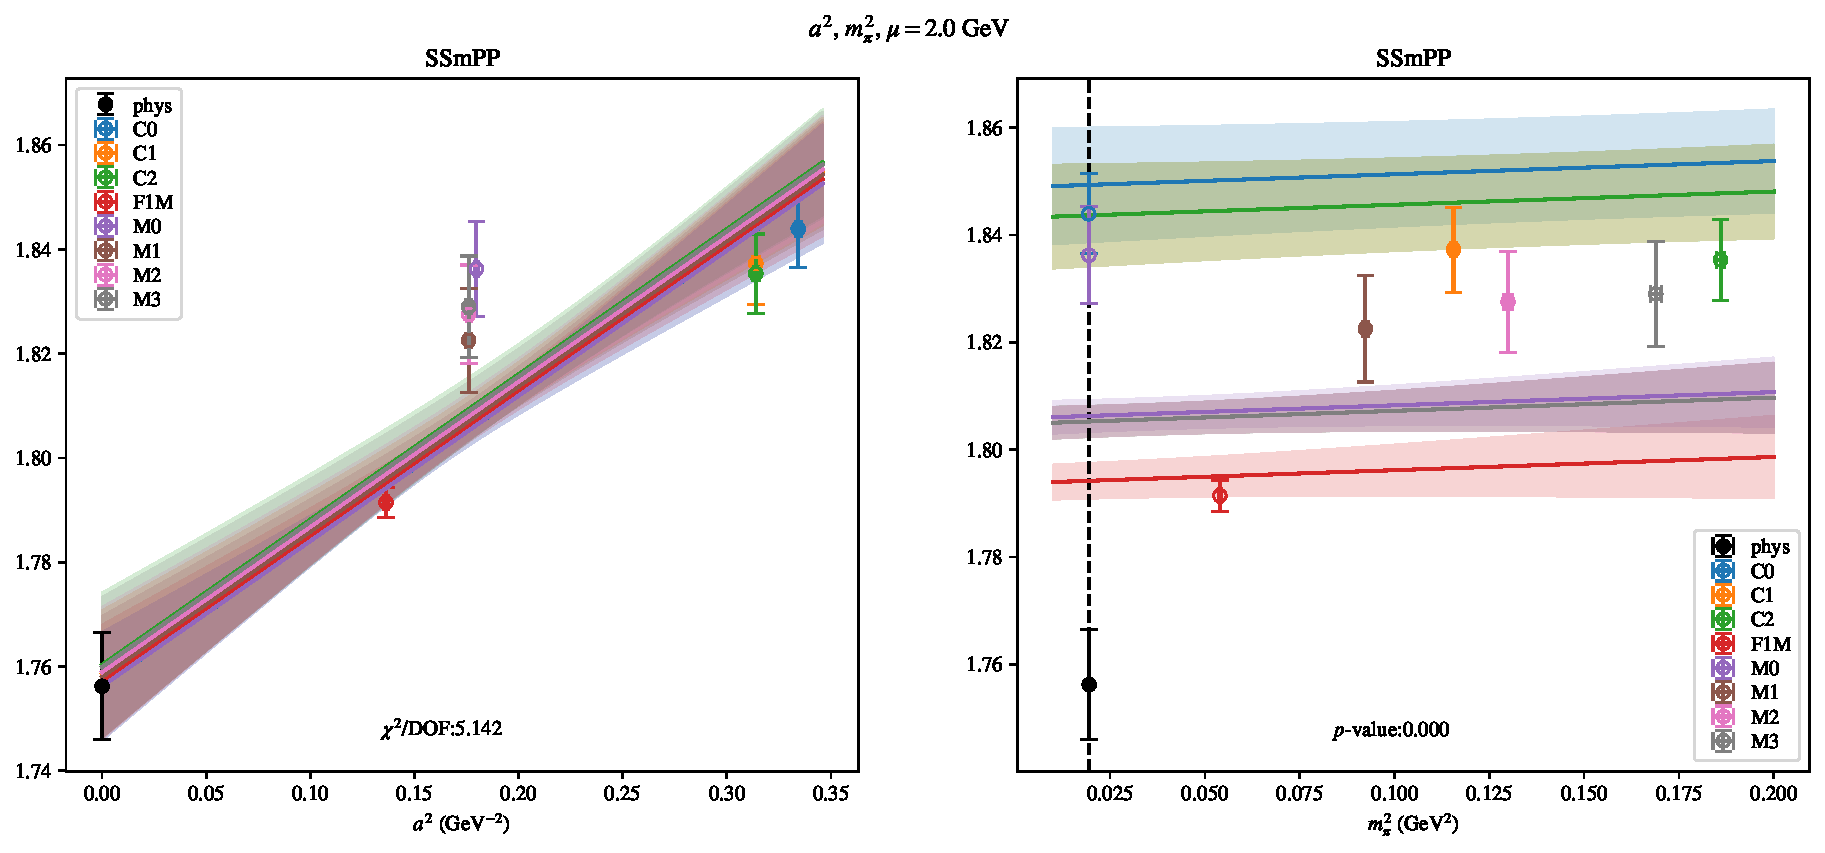
\includepdf[link, pages=-]{SSmPP/NPR/a2m2_20.pdf}
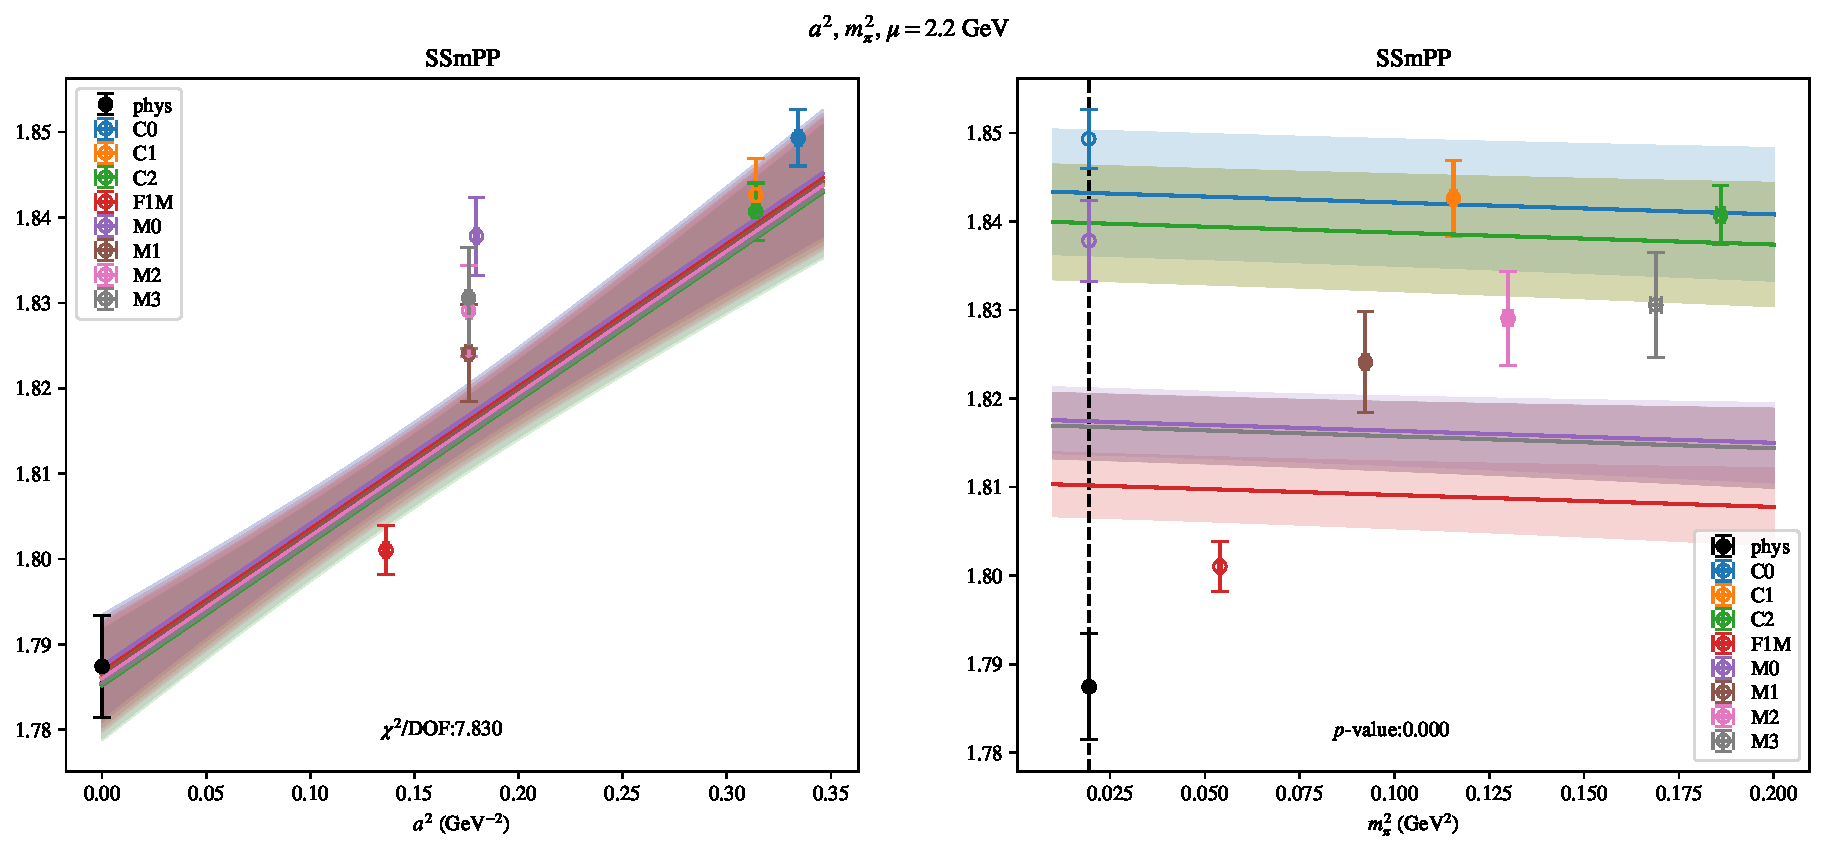
\includepdf[link, pages=-]{SSmPP/NPR/a2m2_22.pdf}
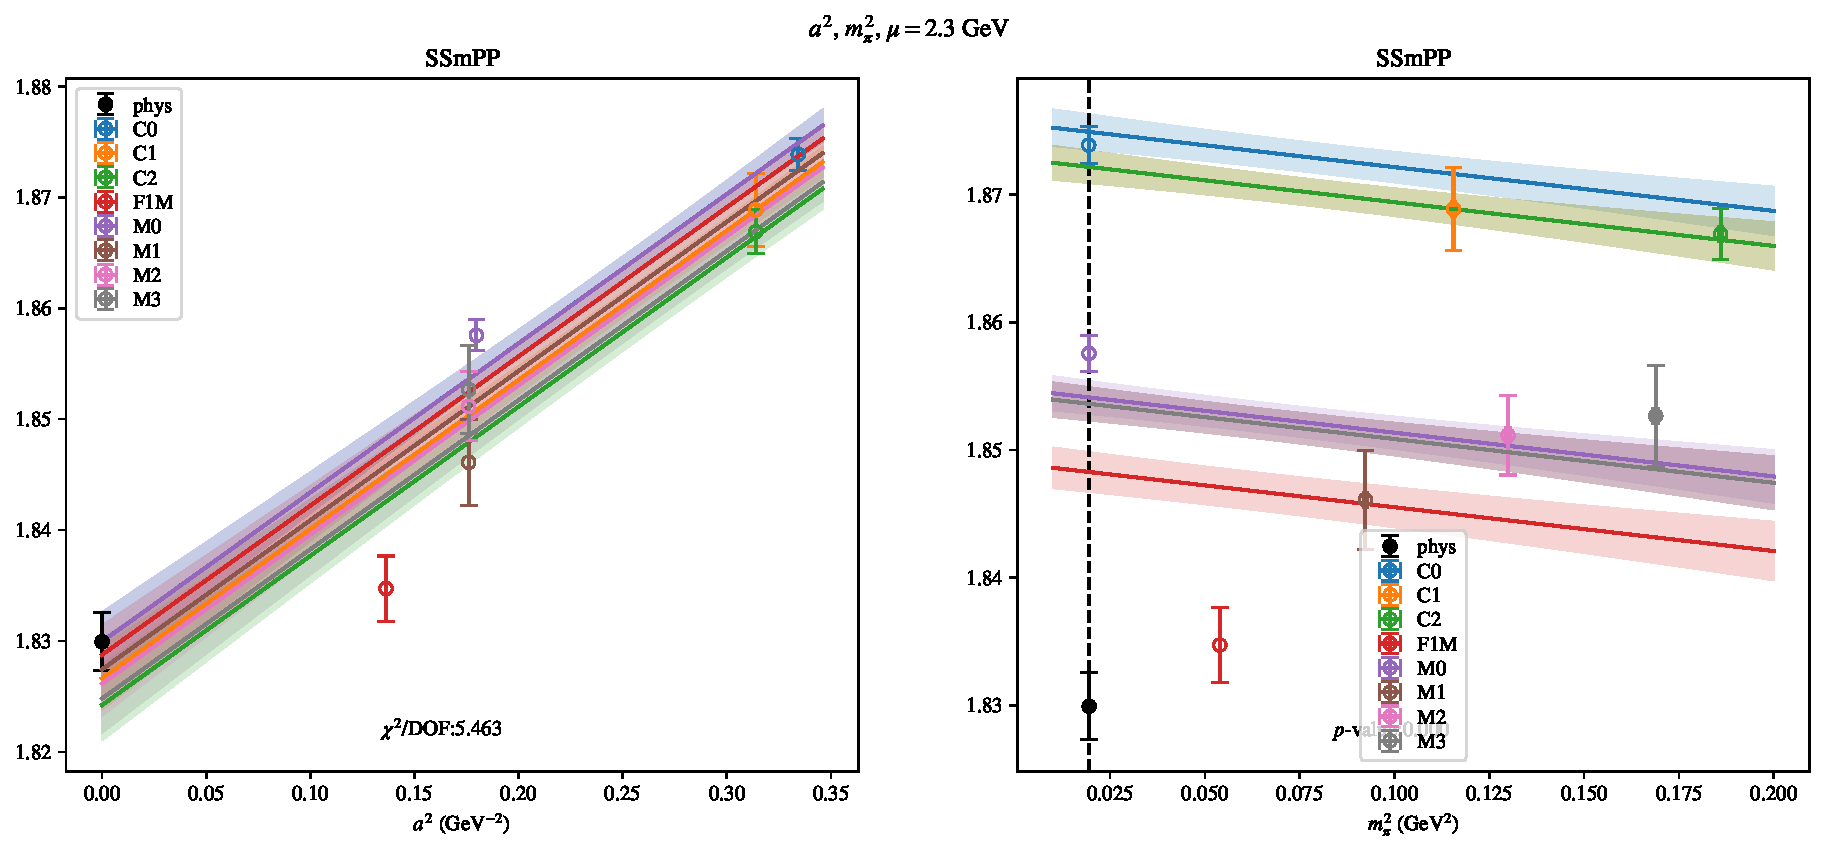
\includepdf[link, pages=-]{SSmPP/NPR/a2m2_23.pdf}
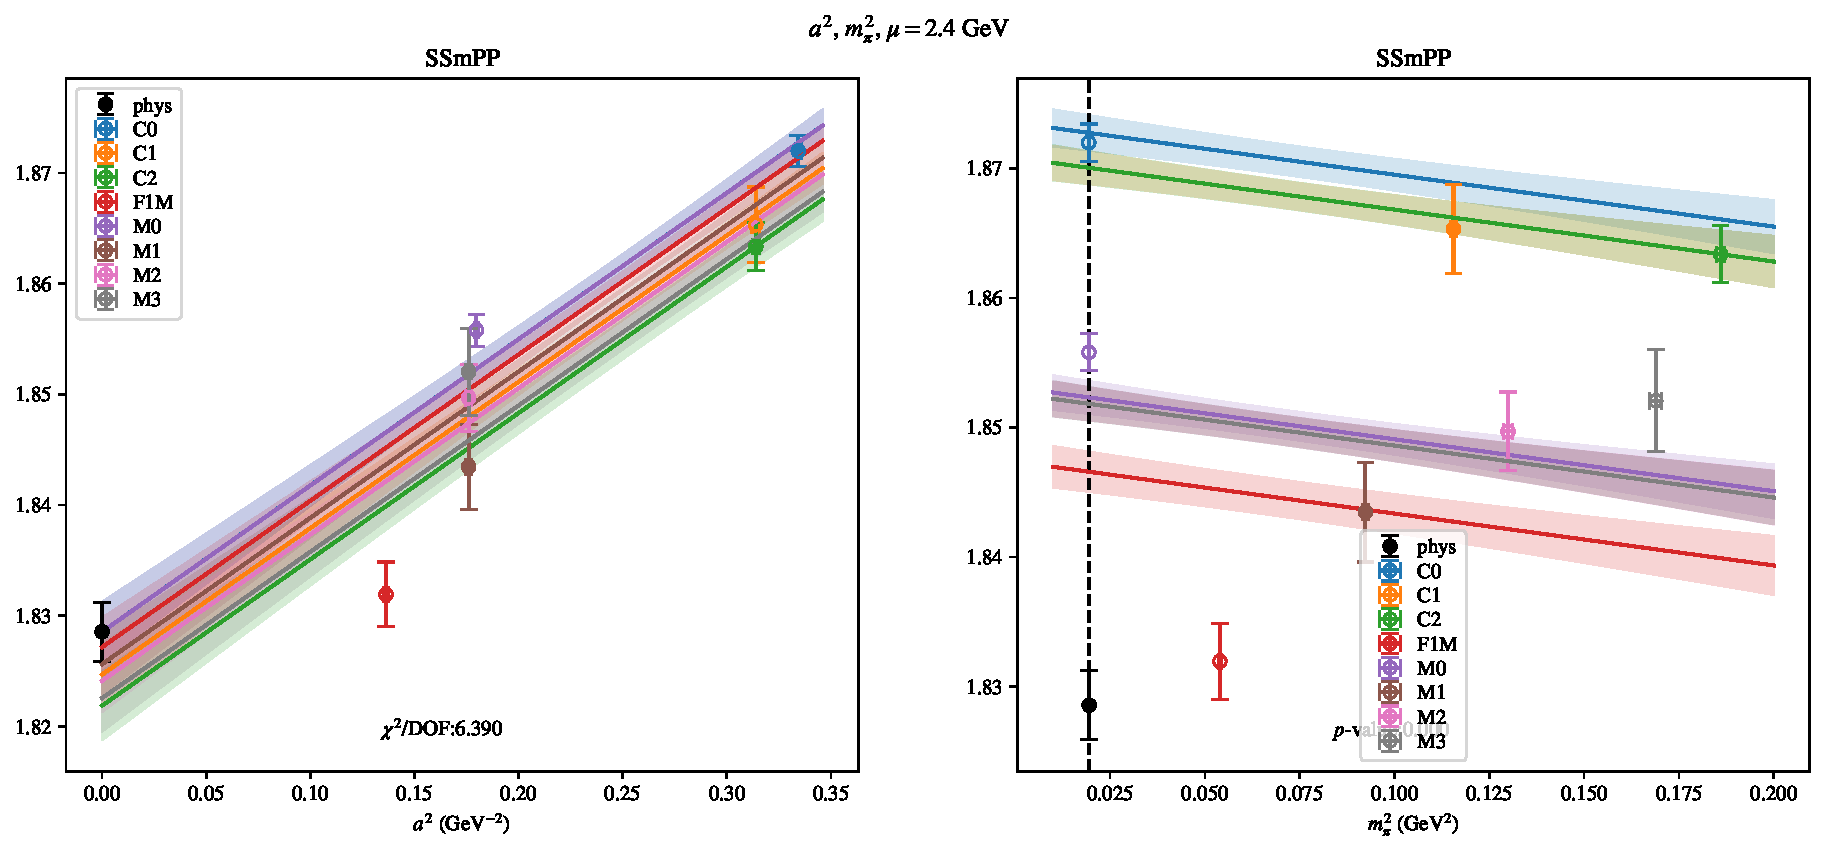
\includepdf[link, pages=-]{SSmPP/NPR/a2m2_24.pdf}
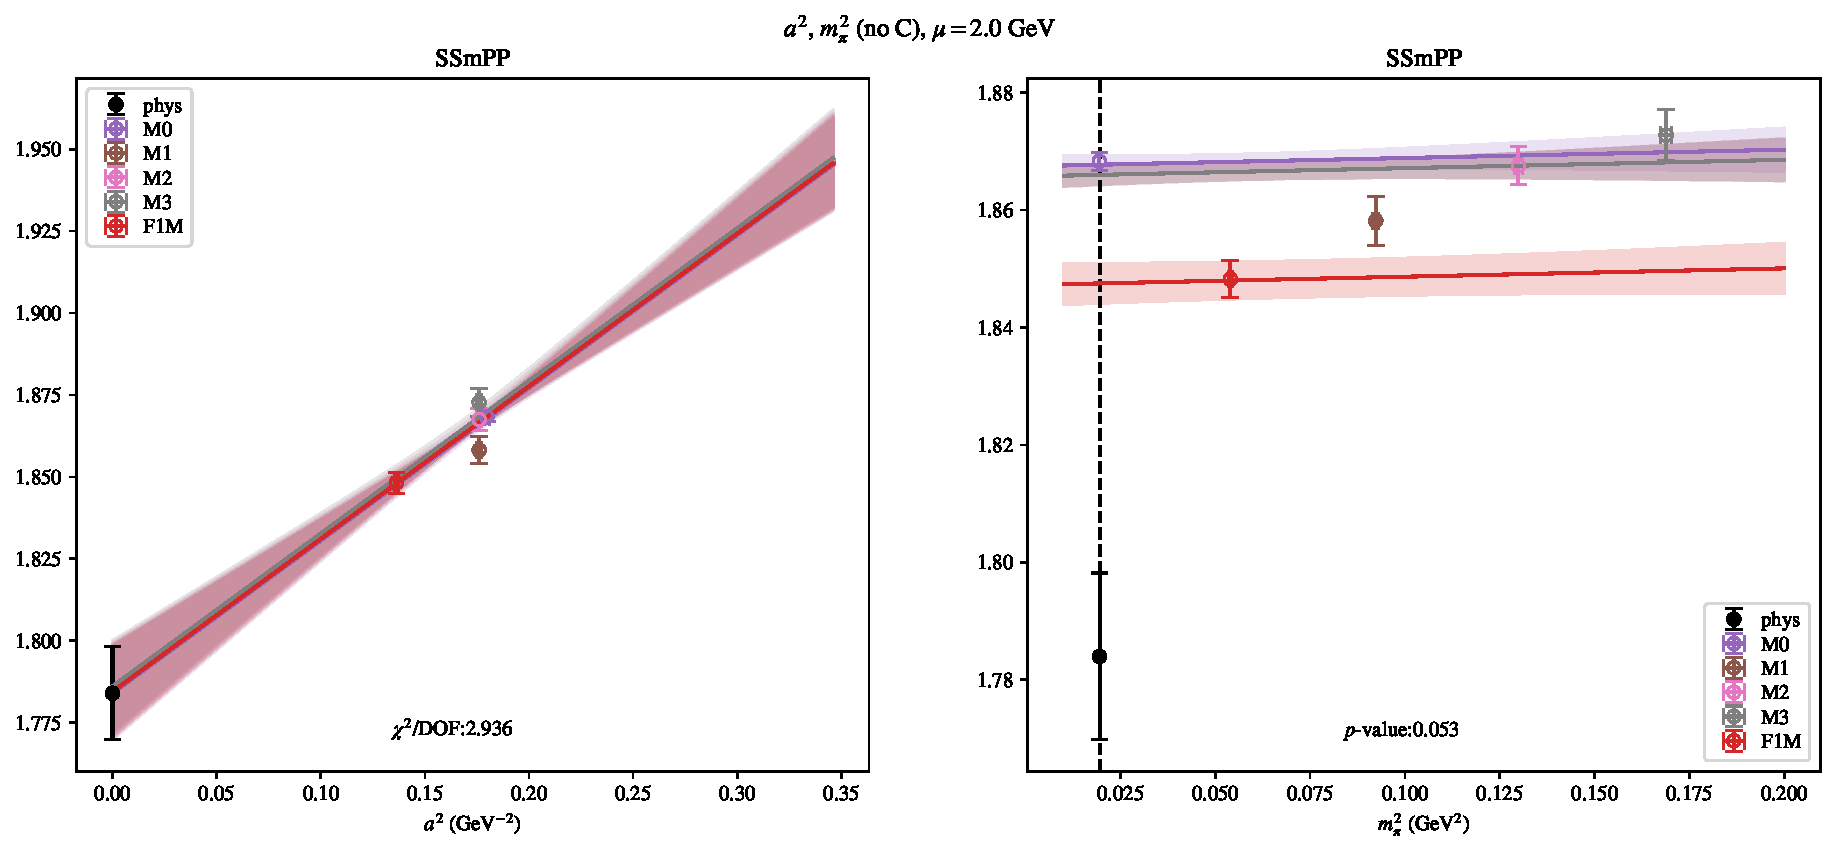
\includepdf[link, pages=-]{SSmPP/NPR/a2m2noC_20.pdf}
\includepdf[link, pages=-]{SSmPP/NPR/a2m2noC_22.pdf}
\includepdf[link, pages=-]{SSmPP/NPR/a2m2noC_23.pdf}
\includepdf[link, pages=-]{SSmPP/NPR/a2m2noC_24.pdf}
\includepdf[link, pages=-]{SSmPP/NPR/a2a4m2_20.pdf}
\includepdf[link, pages=-]{SSmPP/NPR/a2a4m2_22.pdf}
\includepdf[link, pages=-]{SSmPP/NPR/a2a4m2_23.pdf}
\includepdf[link, pages=-]{SSmPP/NPR/a2a4m2_24.pdf}
\includepdf[link, pages=-]{SSmPP/NPR/a2m2mcut_20.pdf}
\includepdf[link, pages=-]{SSmPP/NPR/a2m2mcut_22.pdf}
\includepdf[link, pages=-]{SSmPP/NPR/a2m2mcut_23.pdf}
\includepdf[link, pages=-]{SSmPP/NPR/a2m2mcut_24.pdf}
\includepdf[link, pages=-]{SSmPP/NPR/a2m2m4_20.pdf}
\includepdf[link, pages=-]{SSmPP/NPR/a2m2m4_22.pdf}
\includepdf[link, pages=-]{SSmPP/NPR/a2m2m4_23.pdf}
\includepdf[link, pages=-]{SSmPP/NPR/a2m2m4_24.pdf}
\clearpage
\section{$\mathcal{B}_4$}
\begin{table}[h!]
\begin{center}
\begin{tabular}{|c|c|c|c|c|c|}
\hline
$\mu$ (GeV) & $a^2$, $m_\pi^2$& $a^2$, $m_\pi^2$ (no C)& $a^2$, $a^4$, $m_\pi^2$& $a^2$, $m_\pi^2$ (no M3, C2)& $a^2$, $m_\pi^2$, $m_\pi^4$\\
\hline
2.0& \hyperlink{SSpPP/NPR/a2m2_20.pdf.1}{\textbf{-0.945(23)}: 5.863 (0.0)} & \hyperlink{SSpPP/NPR/a2m2noC_20.pdf.1}{\textbf{-0.990(95)}: 1.747 (0.174)} & \hyperlink{SSpPP/NPR/a2a4m2_20.pdf.1}{\textbf{-0.98(15)}: 5.991 (0.0)} & \hyperlink{SSpPP/NPR/a2m2mcut_20.pdf.1}{\textbf{-0.945(23)}: 7.321 (0.0)} & \hyperlink{SSpPP/NPR/a2m2m4_20.pdf.1}{\textbf{-0.942(23)}: 5.255 (0.0)}\\
2.2& \hyperlink{SSpPP/NPR/a2m2_22.pdf.1}{\textbf{-0.919(20)}: 6.119 (0.0)} & \hyperlink{SSpPP/NPR/a2m2noC_22.pdf.1}{\textbf{-0.957(91)}: 1.941 (0.143)} & \hyperlink{SSpPP/NPR/a2a4m2_22.pdf.1}{\textbf{-0.95(14)}: 6.561 (0.0)} & \hyperlink{SSpPP/NPR/a2m2mcut_22.pdf.1}{\textbf{-0.919(21)}: 7.68 (0.0)} & \hyperlink{SSpPP/NPR/a2m2m4_22.pdf.1}{\textbf{-0.916(21)}: 5.851 (0.0)}\\
2.3& \hyperlink{SSpPP/NPR/a2m2_23.pdf.1}{\textbf{-0.907(19)}: 5.885 (0.0)} & \hyperlink{SSpPP/NPR/a2m2noC_23.pdf.1}{\textbf{-0.945(90)}: 1.895 (0.15)} & \hyperlink{SSpPP/NPR/a2a4m2_23.pdf.1}{\textbf{-0.94(14)}: 6.128 (0.0)} & \hyperlink{SSpPP/NPR/a2m2mcut_23.pdf.1}{\textbf{-0.907(20)}: 7.468 (0.0)} & \hyperlink{SSpPP/NPR/a2m2m4_23.pdf.1}{\textbf{-0.905(20)}: 5.62 (0.0)}\\
2.4& \hyperlink{SSpPP/NPR/a2m2_24.pdf.1}{\textbf{-0.897(19)}: 6.066 (0.0)} & \hyperlink{SSpPP/NPR/a2m2noC_24.pdf.1}{\textbf{-0.932(89)}: 1.814 (0.163)} & \hyperlink{SSpPP/NPR/a2a4m2_24.pdf.1}{\textbf{-0.92(14)}: 6.78 (0.0)} & \hyperlink{SSpPP/NPR/a2m2mcut_24.pdf.1}{\textbf{-0.898(20)}: 7.57 (0.0)} & \hyperlink{SSpPP/NPR/a2m2m4_24.pdf.1}{\textbf{-0.895(20)}: 6.152 (0.0)}\\
\hline
\end{tabular}
\caption{Physical point value from chiral and continuum extrapolation at renormalisation scale $\mu$. Entries are \textbf{value(error)}: $\chi^2/\text{DOF}$ ($p$-value).}
\end{center}
\end{table}
\begin{table}[h!]
\begin{center}
\begin{tabular}{|c c|c|c|c|c|c|}
\hline
$\mu$ (GeV) &  & $a^2$, $m_\pi^2$& $a^2$, $m_\pi^2$ (no C)& $a^2$, $a^4$, $m_\pi^2$& $a^2$, $m_\pi^2$ (no M3, C2)& $a^2$, $m_\pi^2$, $m_\pi^4$\\
\hline
\multirow{2}{0.5in}{2.0} & $\alpha$ & 0.3830(72)& 0.112(55)& -0.023& 0.3816(77)& 0.3937(77)\\
 & $\beta$ & 0.00762(13)& 0.00676(20)& 0.00746(14)& 0.00813(23)& 0.01024(72)\\
\hline
\multirow{2}{0.5in}{2.2} & $\alpha$ & 0.4224(70)& 0.178(56)& 0.079& 0.4199(77)& 0.4322(76)\\
 & $\beta$ & 0.00759(13)& 0.00673(20)& 0.00745(14)& 0.00800(23)& 0.00987(70)\\
\hline
\multirow{2}{0.5in}{2.3} & $\alpha$ & 0.4431(70)& 0.200(56)& 0.09& 0.4410(76)& 0.4523(76)\\
 & $\beta$ & 0.00755(13)& 0.00673(20)& 0.00741(14)& 0.00795(23)& 0.00976(71)\\
\hline
\multirow{2}{0.5in}{2.4} & $\alpha$ & 0.4612(71)& 0.237(56)& 0.17(14)& 0.4578(78)& 0.4696(77)\\
 & $\beta$ & 0.00757(13)& 0.00669(20)& 0.00746(14)& 0.00792(23)& 0.00955(71)\\
\hline
\end{tabular}
\caption{Fit values of coefficients in $Q = Q_{phys} + \mathbf{\alpha} a^2 + \mathbf{\beta}\left(\frac{m_\pi^2}{f_\pi^2}-\frac{m_{\pi,PDG}^2}{f_\pi^2}\right) + \ldots$.}
\end{center}
\end{table}
\includepdf[link, pages=-]{SSpPP/NPR/a2m2_20.pdf}
\includepdf[link, pages=-]{SSpPP/NPR/a2m2_22.pdf}
\includepdf[link, pages=-]{SSpPP/NPR/a2m2_23.pdf}
\includepdf[link, pages=-]{SSpPP/NPR/a2m2_24.pdf}
\includepdf[link, pages=-]{SSpPP/NPR/a2m2noC_20.pdf}
\includepdf[link, pages=-]{SSpPP/NPR/a2m2noC_22.pdf}
\includepdf[link, pages=-]{SSpPP/NPR/a2m2noC_23.pdf}
\includepdf[link, pages=-]{SSpPP/NPR/a2m2noC_24.pdf}
\includepdf[link, pages=-]{SSpPP/NPR/a2a4m2_20.pdf}
\includepdf[link, pages=-]{SSpPP/NPR/a2a4m2_22.pdf}
\includepdf[link, pages=-]{SSpPP/NPR/a2a4m2_23.pdf}
\includepdf[link, pages=-]{SSpPP/NPR/a2a4m2_24.pdf}
\includepdf[link, pages=-]{SSpPP/NPR/a2m2mcut_20.pdf}
\includepdf[link, pages=-]{SSpPP/NPR/a2m2mcut_22.pdf}
\includepdf[link, pages=-]{SSpPP/NPR/a2m2mcut_23.pdf}
\includepdf[link, pages=-]{SSpPP/NPR/a2m2mcut_24.pdf}
\includepdf[link, pages=-]{SSpPP/NPR/a2m2m4_20.pdf}
\includepdf[link, pages=-]{SSpPP/NPR/a2m2m4_22.pdf}
\includepdf[link, pages=-]{SSpPP/NPR/a2m2m4_23.pdf}
\includepdf[link, pages=-]{SSpPP/NPR/a2m2m4_24.pdf}
\clearpage
\section{$\mathcal{B}_5$}
\begin{table}[h!]
\begin{center}
\begin{tabular}{|c|c|c|c|c|c|}
\hline
$\mu$ (GeV) & $a^2$, $m_\pi^2$& $a^2$, $m_\pi^2$ (no C)& $a^2$, $a^4$, $m_\pi^2$& $a^2$, $m_\pi^2$ (no M3, C2)& $a^2$, $m_\pi^2$, $m_\pi^4$\\
\hline
2.0& \hyperlink{TT/NPR/a2m2_20.pdf.1}{\textbf{-0.369(12)}: 1.702 (0.13)} & \hyperlink{TT/NPR/a2m2noC_20.pdf.1}{\textbf{-0.386(48)}: 0.214 (0.807)} & \hyperlink{TT/NPR/a2a4m2_20.pdf.1}{\textbf{-0.384(77)}: 1.721 (0.142)} & \hyperlink{TT/NPR/a2m2mcut_20.pdf.1}{\textbf{-0.370(11)}: 2.378 (0.068)} & \hyperlink{TT/NPR/a2m2m4_20.pdf.1}{\textbf{-0.369(11)}: 1.959 (0.098)}\\
2.2& \hyperlink{TT/NPR/a2m2_22.pdf.1}{\textbf{-0.3646(88)}: 2.078 (0.065)} & \hyperlink{TT/NPR/a2m2noC_22.pdf.1}{\textbf{-0.377(40)}: 0.382 (0.682)} & \hyperlink{TT/NPR/a2a4m2_22.pdf.1}{\textbf{-0.377(64)}: 1.995 (0.092)} & \hyperlink{TT/NPR/a2m2mcut_22.pdf.1}{\textbf{-0.3650(87)}: 2.978 (0.03)} & \hyperlink{TT/NPR/a2m2m4_22.pdf.1}{\textbf{-0.3643(84)}: 2.427 (0.046)}\\
2.3& \hyperlink{TT/NPR/a2m2_23.pdf.1}{\textbf{-0.3626(80)}: 1.833 (0.103)} & \hyperlink{TT/NPR/a2m2noC_23.pdf.1}{\textbf{-0.374(39)}: 0.428 (0.652)} & \hyperlink{TT/NPR/a2a4m2_23.pdf.1}{\textbf{-0.374(62)}: 1.731 (0.14)} & \hyperlink{TT/NPR/a2m2mcut_23.pdf.1}{\textbf{-0.3629(80)}: 2.671 (0.046)} & \hyperlink{TT/NPR/a2m2m4_23.pdf.1}{\textbf{-0.3622(78)}: 2.102 (0.078)}\\
2.4& \hyperlink{TT/NPR/a2m2_24.pdf.1}{\textbf{-0.3609(78)}: 1.62 (0.151)} & \hyperlink{TT/NPR/a2m2noC_24.pdf.1}{\textbf{-0.370(39)}: 0.457 (0.633)} & \hyperlink{TT/NPR/a2a4m2_24.pdf.1}{\textbf{-0.370(61)}: 1.651 (0.158)} & \hyperlink{TT/NPR/a2m2mcut_24.pdf.1}{\textbf{-0.3611(77)}: 2.357 (0.07)} & \hyperlink{TT/NPR/a2m2m4_24.pdf.1}{\textbf{-0.3606(76)}: 1.866 (0.113)}\\
\hline
\end{tabular}
\caption{Physical point value from chiral and continuum extrapolation at renormalisation scale $\mu$. Entries are \textbf{value(error)}: $\chi^2/\text{DOF}$ ($p$-value).}
\end{center}
\end{table}
\begin{table}[h!]
\begin{center}
\begin{tabular}{|c c|c|c|c|c|c|}
\hline
$\mu$ (GeV) &  & $a^2$, $m_\pi^2$& $a^2$, $m_\pi^2$ (no C)& $a^2$, $a^4$, $m_\pi^2$& $a^2$, $m_\pi^2$ (no M3, C2)& $a^2$, $m_\pi^2$, $m_\pi^4$\\
\hline
\multirow{2}{0.5in}{2.0} & $\alpha$ & -0.027(74)& -0.25(64)& -0.3(16)& -0.031(72)& -0.024(71)\\
 & $\beta$ & 0.00702(15)& 0.00612(26)& 0.00689(14)& 0.00716(27)& 0.00808(80)\\
\hline
\multirow{2}{0.5in}{2.2} & $\alpha$ & -0.076(60)& -0.26(57)& -0.3(14)& -0.081(65)& -0.074(63)\\
 & $\beta$ & 0.00673(12)& 0.00604(20)& 0.00662(13)& 0.00680(21)& 0.00759(65)\\
\hline
\multirow{2}{0.5in}{2.3} & $\alpha$ & -0.102(58)& -0.27(57)& -0.3(14)& -0.105(63)& -0.099(61)\\
 & $\beta$ & 0.00666(12)& 0.00606(20)& 0.00656(13)& 0.00674(21)& 0.00753(64)\\
\hline
\multirow{2}{0.5in}{2.4} & $\alpha$ & -0.127(58)& -0.27(57)& -0.3(14)& -0.130(62)& -0.124(60)\\
 & $\beta$ & 0.00658(12)& 0.00603(20)& 0.00650(12)& 0.00665(20)& 0.00734(63)\\
\hline
\end{tabular}
\caption{Fit values of coefficients in $Q = Q_{phys} + \mathbf{\alpha} a^2 + \mathbf{\beta}\left(\frac{m_\pi^2}{f_\pi^2}-\frac{m_{\pi,PDG}^2}{f_\pi^2}\right) + \ldots$.}
\end{center}
\end{table}
\includepdf[link, pages=-]{TT/NPR/a2m2_20.pdf}
\includepdf[link, pages=-]{TT/NPR/a2m2_22.pdf}
\includepdf[link, pages=-]{TT/NPR/a2m2_23.pdf}
\includepdf[link, pages=-]{TT/NPR/a2m2_24.pdf}
\includepdf[link, pages=-]{TT/NPR/a2m2noC_20.pdf}
\includepdf[link, pages=-]{TT/NPR/a2m2noC_22.pdf}
\includepdf[link, pages=-]{TT/NPR/a2m2noC_23.pdf}
\includepdf[link, pages=-]{TT/NPR/a2m2noC_24.pdf}
\includepdf[link, pages=-]{TT/NPR/a2a4m2_20.pdf}
\includepdf[link, pages=-]{TT/NPR/a2a4m2_22.pdf}
\includepdf[link, pages=-]{TT/NPR/a2a4m2_23.pdf}
\includepdf[link, pages=-]{TT/NPR/a2a4m2_24.pdf}
\includepdf[link, pages=-]{TT/NPR/a2m2mcut_20.pdf}
\includepdf[link, pages=-]{TT/NPR/a2m2mcut_22.pdf}
\includepdf[link, pages=-]{TT/NPR/a2m2mcut_23.pdf}
\includepdf[link, pages=-]{TT/NPR/a2m2mcut_24.pdf}
\includepdf[link, pages=-]{TT/NPR/a2m2m4_20.pdf}
\includepdf[link, pages=-]{TT/NPR/a2m2m4_22.pdf}
\includepdf[link, pages=-]{TT/NPR/a2m2m4_23.pdf}
\includepdf[link, pages=-]{TT/NPR/a2m2m4_24.pdf}
\clearpage
\end{document}